\documentclass[twoside]{book}

% Packages required by doxygen
\usepackage{fixltx2e}
\usepackage{calc}
\usepackage{doxygen}
\usepackage[export]{adjustbox} % also loads graphicx
\usepackage{graphicx}
\usepackage[utf8]{inputenc}
\usepackage{makeidx}
\usepackage{multicol}
\usepackage{multirow}
\PassOptionsToPackage{warn}{textcomp}
\usepackage{textcomp}
\usepackage[nointegrals]{wasysym}
\usepackage[table]{xcolor}

% Font selection
\usepackage[T1]{fontenc}
\usepackage[scaled=.90]{helvet}
\usepackage{courier}
\usepackage{amssymb}
\usepackage{sectsty}
\renewcommand{\familydefault}{\sfdefault}
\allsectionsfont{%
  \fontseries{bc}\selectfont%
  \color{darkgray}%
}
\renewcommand{\DoxyLabelFont}{%
  \fontseries{bc}\selectfont%
  \color{darkgray}%
}
\newcommand{\+}{\discretionary{\mbox{\scriptsize$\hookleftarrow$}}{}{}}

% Page & text layout
\usepackage{geometry}
\geometry{%
  a4paper,%
  top=2.5cm,%
  bottom=2.5cm,%
  left=2.5cm,%
  right=2.5cm%
}
\tolerance=750
\hfuzz=15pt
\hbadness=750
\setlength{\emergencystretch}{15pt}
\setlength{\parindent}{0cm}
\setlength{\parskip}{3ex plus 2ex minus 2ex}
\makeatletter
\renewcommand{\paragraph}{%
  \@startsection{paragraph}{4}{0ex}{-1.0ex}{1.0ex}{%
    \normalfont\normalsize\bfseries\SS@parafont%
  }%
}
\renewcommand{\subparagraph}{%
  \@startsection{subparagraph}{5}{0ex}{-1.0ex}{1.0ex}{%
    \normalfont\normalsize\bfseries\SS@subparafont%
  }%
}
\makeatother

% Headers & footers
\usepackage{fancyhdr}
\pagestyle{fancyplain}
\fancyhead[LE]{\fancyplain{}{\bfseries\thepage}}
\fancyhead[CE]{\fancyplain{}{}}
\fancyhead[RE]{\fancyplain{}{\bfseries\leftmark}}
\fancyhead[LO]{\fancyplain{}{\bfseries\rightmark}}
\fancyhead[CO]{\fancyplain{}{}}
\fancyhead[RO]{\fancyplain{}{\bfseries\thepage}}
\fancyfoot[LE]{\fancyplain{}{}}
\fancyfoot[CE]{\fancyplain{}{}}
\fancyfoot[RE]{\fancyplain{}{\bfseries\scriptsize Generated by Doxygen }}
\fancyfoot[LO]{\fancyplain{}{\bfseries\scriptsize Generated by Doxygen }}
\fancyfoot[CO]{\fancyplain{}{}}
\fancyfoot[RO]{\fancyplain{}{}}
\renewcommand{\footrulewidth}{0.4pt}
\renewcommand{\chaptermark}[1]{%
  \markboth{#1}{}%
}
\renewcommand{\sectionmark}[1]{%
  \markright{\thesection\ #1}%
}

% Indices & bibliography
\usepackage{natbib}
\usepackage[titles]{tocloft}
\setcounter{tocdepth}{3}
\setcounter{secnumdepth}{5}
\makeindex

% Hyperlinks (required, but should be loaded last)
\usepackage{ifpdf}
\ifpdf
  \usepackage[pdftex,pagebackref=true]{hyperref}
\else
  \usepackage[ps2pdf,pagebackref=true]{hyperref}
\fi
\hypersetup{%
  colorlinks=true,%
  linkcolor=blue,%
  citecolor=blue,%
  unicode%
}

% Custom commands
\newcommand{\clearemptydoublepage}{%
  \newpage{\pagestyle{empty}\cleardoublepage}%
}

\usepackage{caption}
\captionsetup{labelsep=space,justification=centering,font={bf},singlelinecheck=off,skip=4pt,position=top}

%===== C O N T E N T S =====

\begin{document}

% Titlepage & ToC
\hypersetup{pageanchor=false,
             bookmarksnumbered=true,
             pdfencoding=unicode
            }
\pagenumbering{alph}
\begin{titlepage}
\vspace*{7cm}
\begin{center}%
{\Large Lurrun Doxygen }\\
\vspace*{1cm}
{\large Generated by Doxygen 1.8.13}\\
\end{center}
\end{titlepage}
\clearemptydoublepage
\pagenumbering{roman}
\tableofcontents
\clearemptydoublepage
\pagenumbering{arabic}
\hypersetup{pageanchor=true}

%--- Begin generated contents ---
\chapter{Namespace Index}
\section{Packages}
Here are the packages with brief descriptions (if available)\+:\begin{DoxyCompactList}
\item\contentsline{section}{\hyperlink{namespacees}{es} }{\pageref{namespacees}}{}
\item\contentsline{section}{\hyperlink{namespacees_1_1deusto}{es.\+deusto} }{\pageref{namespacees_1_1deusto}}{}
\item\contentsline{section}{\hyperlink{namespacees_1_1deusto_1_1client}{es.\+deusto.\+client} }{\pageref{namespacees_1_1deusto_1_1client}}{}
\item\contentsline{section}{\hyperlink{namespacees_1_1deusto_1_1server}{es.\+deusto.\+server} }{\pageref{namespacees_1_1deusto_1_1server}}{}
\item\contentsline{section}{\hyperlink{namespacees_1_1deusto_1_1server_1_1db}{es.\+deusto.\+server.\+db} }{\pageref{namespacees_1_1deusto_1_1server_1_1db}}{}
\item\contentsline{section}{\hyperlink{namespacees_1_1deusto_1_1server_1_1db_1_1dao}{es.\+deusto.\+server.\+db.\+dao} }{\pageref{namespacees_1_1deusto_1_1server_1_1db_1_1dao}}{}
\item\contentsline{section}{\hyperlink{namespacees_1_1deusto_1_1server_1_1db_1_1data}{es.\+deusto.\+server.\+db.\+data} }{\pageref{namespacees_1_1deusto_1_1server_1_1db_1_1data}}{}
\item\contentsline{section}{\hyperlink{namespacees_1_1deusto_1_1server_1_1remote}{es.\+deusto.\+server.\+remote} }{\pageref{namespacees_1_1deusto_1_1server_1_1remote}}{}
\end{DoxyCompactList}

\chapter{Hierarchical Index}
\section{Class Hierarchy}
This inheritance list is sorted roughly, but not completely, alphabetically\+:\begin{DoxyCompactList}
\item \contentsline{section}{es.\+deusto.\+client.\+Client}{\pageref{classes_1_1deusto_1_1client_1_1_client}}{}
\item \contentsline{section}{es.\+deusto.\+server.\+db.\+dao.\+I\+D\+AO}{\pageref{interfacees_1_1deusto_1_1server_1_1db_1_1dao_1_1_i_d_a_o}}{}
\begin{DoxyCompactList}
\item \contentsline{section}{es.\+deusto.\+server.\+db.\+dao.\+D\+AO}{\pageref{classes_1_1deusto_1_1server_1_1db_1_1dao_1_1_d_a_o}}{}
\end{DoxyCompactList}
\item \contentsline{section}{es.\+deusto.\+server.\+db.\+I\+DB}{\pageref{interfacees_1_1deusto_1_1server_1_1db_1_1_i_d_b}}{}
\begin{DoxyCompactList}
\item \contentsline{section}{es.\+deusto.\+server.\+db.\+DB}{\pageref{classes_1_1deusto_1_1server_1_1db_1_1_d_b}}{}
\end{DoxyCompactList}
\item \contentsline{section}{es.\+deusto.\+server.\+remote.\+I\+Remote}{\pageref{interfacees_1_1deusto_1_1server_1_1remote_1_1_i_remote}}{}
\begin{DoxyCompactList}
\item \contentsline{section}{es.\+deusto.\+server.\+remote.\+Remote}{\pageref{classes_1_1deusto_1_1server_1_1remote_1_1_remote}}{}
\end{DoxyCompactList}
\item \contentsline{section}{es.\+deusto.\+server.\+Server}{\pageref{classes_1_1deusto_1_1server_1_1_server}}{}
\item Serializable\begin{DoxyCompactList}
\item \contentsline{section}{es.\+deusto.\+server.\+db.\+data.\+Company}{\pageref{classes_1_1deusto_1_1server_1_1db_1_1data_1_1_company}}{}
\item \contentsline{section}{es.\+deusto.\+server.\+db.\+data.\+Game}{\pageref{classes_1_1deusto_1_1server_1_1db_1_1data_1_1_game}}{}
\item \contentsline{section}{es.\+deusto.\+server.\+db.\+data.\+Genre}{\pageref{classes_1_1deusto_1_1server_1_1db_1_1data_1_1_genre}}{}
\item \contentsline{section}{es.\+deusto.\+server.\+db.\+data.\+License}{\pageref{classes_1_1deusto_1_1server_1_1db_1_1data_1_1_license}}{}
\item \contentsline{section}{es.\+deusto.\+server.\+db.\+data.\+User}{\pageref{classes_1_1deusto_1_1server_1_1db_1_1data_1_1_user}}{}
\end{DoxyCompactList}
\item Unicast\+Remote\+Object\begin{DoxyCompactList}
\item \contentsline{section}{es.\+deusto.\+server.\+remote.\+Remote}{\pageref{classes_1_1deusto_1_1server_1_1remote_1_1_remote}}{}
\end{DoxyCompactList}
\end{DoxyCompactList}

\chapter{Class Index}
\section{Class List}
Here are the classes, structs, unions and interfaces with brief descriptions\+:\begin{DoxyCompactList}
\item\contentsline{section}{\hyperlink{classes_1_1deusto_1_1client_1_1_client}{es.\+deusto.\+client.\+Client} }{\pageref{classes_1_1deusto_1_1client_1_1_client}}{}
\item\contentsline{section}{\hyperlink{classes_1_1deusto_1_1server_1_1db_1_1data_1_1_company}{es.\+deusto.\+server.\+db.\+data.\+Company} }{\pageref{classes_1_1deusto_1_1server_1_1db_1_1data_1_1_company}}{}
\item\contentsline{section}{\hyperlink{classes_1_1deusto_1_1server_1_1db_1_1dao_1_1_d_a_o}{es.\+deusto.\+server.\+db.\+dao.\+D\+AO} }{\pageref{classes_1_1deusto_1_1server_1_1db_1_1dao_1_1_d_a_o}}{}
\item\contentsline{section}{\hyperlink{classes_1_1deusto_1_1server_1_1_d_a_o_mock_test}{es.\+deusto.\+server.\+D\+A\+O\+Mock\+Test} }{\pageref{classes_1_1deusto_1_1server_1_1_d_a_o_mock_test}}{}
\item\contentsline{section}{\hyperlink{classes_1_1deusto_1_1server_1_1db_1_1_d_b}{es.\+deusto.\+server.\+db.\+DB} }{\pageref{classes_1_1deusto_1_1server_1_1db_1_1_d_b}}{}
\item\contentsline{section}{\hyperlink{classes_1_1deusto_1_1server_1_1db_1_1data_1_1_game}{es.\+deusto.\+server.\+db.\+data.\+Game} }{\pageref{classes_1_1deusto_1_1server_1_1db_1_1data_1_1_game}}{}
\item\contentsline{section}{\hyperlink{classes_1_1deusto_1_1server_1_1db_1_1data_1_1_genre}{es.\+deusto.\+server.\+db.\+data.\+Genre} }{\pageref{classes_1_1deusto_1_1server_1_1db_1_1data_1_1_genre}}{}
\item\contentsline{section}{\hyperlink{interfacees_1_1deusto_1_1server_1_1db_1_1dao_1_1_i_d_a_o}{es.\+deusto.\+server.\+db.\+dao.\+I\+D\+AO} }{\pageref{interfacees_1_1deusto_1_1server_1_1db_1_1dao_1_1_i_d_a_o}}{}
\item\contentsline{section}{\hyperlink{interfacees_1_1deusto_1_1server_1_1db_1_1_i_d_b}{es.\+deusto.\+server.\+db.\+I\+DB} }{\pageref{interfacees_1_1deusto_1_1server_1_1db_1_1_i_d_b}}{}
\item\contentsline{section}{\hyperlink{interfacees_1_1deusto_1_1server_1_1remote_1_1_i_remote}{es.\+deusto.\+server.\+remote.\+I\+Remote} }{\pageref{interfacees_1_1deusto_1_1server_1_1remote_1_1_i_remote}}{}
\item\contentsline{section}{\hyperlink{classes_1_1deusto_1_1server_1_1db_1_1data_1_1_license}{es.\+deusto.\+server.\+db.\+data.\+License} }{\pageref{classes_1_1deusto_1_1server_1_1db_1_1data_1_1_license}}{}
\item\contentsline{section}{\hyperlink{classes_1_1deusto_1_1server_1_1remote_1_1_remote}{es.\+deusto.\+server.\+remote.\+Remote} }{\pageref{classes_1_1deusto_1_1server_1_1remote_1_1_remote}}{}
\item\contentsline{section}{\hyperlink{classes_1_1deusto_1_1server_1_1_r_m_i_test}{es.\+deusto.\+server.\+R\+M\+I\+Test} }{\pageref{classes_1_1deusto_1_1server_1_1_r_m_i_test}}{}
\item\contentsline{section}{\hyperlink{classes_1_1deusto_1_1server_1_1_server}{es.\+deusto.\+server.\+Server} }{\pageref{classes_1_1deusto_1_1server_1_1_server}}{}
\item\contentsline{section}{\hyperlink{classes_1_1deusto_1_1server_1_1db_1_1data_1_1_user}{es.\+deusto.\+server.\+db.\+data.\+User} }{\pageref{classes_1_1deusto_1_1server_1_1db_1_1data_1_1_user}}{}
\end{DoxyCompactList}

\chapter{File Index}
\section{File List}
Here is a list of all files with brief descriptions\+:\begin{DoxyCompactList}
\item\contentsline{section}{src/main/java/es/deusto/client/\hyperlink{_client_8java}{Client.\+java} }{\pageref{_client_8java}}{}
\item\contentsline{section}{src/main/java/es/deusto/client/\hyperlink{_g_u_i_8java}{G\+U\+I.\+java} }{\pageref{_g_u_i_8java}}{}
\item\contentsline{section}{src/main/java/es/deusto/server/\hyperlink{_server_8java}{Server.\+java} }{\pageref{_server_8java}}{}
\item\contentsline{section}{src/main/java/es/deusto/server/db/\hyperlink{_d_b_8java}{D\+B.\+java} }{\pageref{_d_b_8java}}{}
\item\contentsline{section}{src/main/java/es/deusto/server/db/\hyperlink{_i_d_b_8java}{I\+D\+B.\+java} }{\pageref{_i_d_b_8java}}{}
\item\contentsline{section}{src/main/java/es/deusto/server/db/dao/\hyperlink{_d_a_o_8java}{D\+A\+O.\+java} }{\pageref{_d_a_o_8java}}{}
\item\contentsline{section}{src/main/java/es/deusto/server/db/dao/\hyperlink{_i_d_a_o_8java}{I\+D\+A\+O.\+java} }{\pageref{_i_d_a_o_8java}}{}
\item\contentsline{section}{src/main/java/es/deusto/server/db/data/\hyperlink{_company_8java}{Company.\+java} }{\pageref{_company_8java}}{}
\item\contentsline{section}{src/main/java/es/deusto/server/db/data/\hyperlink{_game_8java}{Game.\+java} }{\pageref{_game_8java}}{}
\item\contentsline{section}{src/main/java/es/deusto/server/db/data/\hyperlink{_genre_8java}{Genre.\+java} }{\pageref{_genre_8java}}{}
\item\contentsline{section}{src/main/java/es/deusto/server/db/data/\hyperlink{_license_8java}{License.\+java} }{\pageref{_license_8java}}{}
\item\contentsline{section}{src/main/java/es/deusto/server/db/data/\hyperlink{_user_8java}{User.\+java} }{\pageref{_user_8java}}{}
\item\contentsline{section}{src/main/java/es/deusto/server/remote/\hyperlink{_i_remote_8java}{I\+Remote.\+java} }{\pageref{_i_remote_8java}}{}
\item\contentsline{section}{src/main/java/es/deusto/server/remote/\hyperlink{_remote_8java}{Remote.\+java} }{\pageref{_remote_8java}}{}
\item\contentsline{section}{src/test/java/es/deusto/server/\hyperlink{_conti_perf_test_8java}{Conti\+Perf\+Test.\+java} }{\pageref{_conti_perf_test_8java}}{}
\item\contentsline{section}{src/test/java/es/deusto/server/\hyperlink{_d_a_o_mock_test_8java}{D\+A\+O\+Mock\+Test.\+java} }{\pageref{_d_a_o_mock_test_8java}}{}
\item\contentsline{section}{src/test/java/es/deusto/server/\hyperlink{_r_m_i_test_8java}{R\+M\+I\+Test.\+java} }{\pageref{_r_m_i_test_8java}}{}
\end{DoxyCompactList}

\chapter{Namespace Documentation}
\hypertarget{namespacees}{}\section{Package es}
\label{namespacees}\index{es@{es}}
\subsection*{Packages}
\begin{DoxyCompactItemize}
\item 
package \hyperlink{namespacees_1_1deusto}{deusto}
\end{DoxyCompactItemize}

\hypertarget{namespacees_1_1deusto}{}\section{Package es.\+deusto}
\label{namespacees_1_1deusto}\index{es.\+deusto@{es.\+deusto}}
\subsection*{Packages}
\begin{DoxyCompactItemize}
\item 
package \hyperlink{namespacees_1_1deusto_1_1client}{client}
\item 
package \hyperlink{namespacees_1_1deusto_1_1server}{server}
\end{DoxyCompactItemize}

\hypertarget{namespacees_1_1deusto_1_1client}{}\section{Package es.\+deusto.\+client}
\label{namespacees_1_1deusto_1_1client}\index{es.\+deusto.\+client@{es.\+deusto.\+client}}
\subsection*{Classes}
\begin{DoxyCompactItemize}
\item 
class \hyperlink{classes_1_1deusto_1_1client_1_1_client}{Client}
\item 
class \hyperlink{classes_1_1deusto_1_1client_1_1_g_u_i}{G\+UI}
\end{DoxyCompactItemize}

\hypertarget{namespacees_1_1deusto_1_1server}{}\section{Package es.\+deusto.\+server}
\label{namespacees_1_1deusto_1_1server}\index{es.\+deusto.\+server@{es.\+deusto.\+server}}
\subsection*{Packages}
\begin{DoxyCompactItemize}
\item 
package \hyperlink{namespacees_1_1deusto_1_1server_1_1db}{db}
\item 
package \hyperlink{namespacees_1_1deusto_1_1server_1_1remote}{remote}
\end{DoxyCompactItemize}
\subsection*{Classes}
\begin{DoxyCompactItemize}
\item 
class \hyperlink{classes_1_1deusto_1_1server_1_1_server}{Server}
\end{DoxyCompactItemize}

\hypertarget{namespacees_1_1deusto_1_1server_1_1db}{}\section{Package es.\+deusto.\+server.\+db}
\label{namespacees_1_1deusto_1_1server_1_1db}\index{es.\+deusto.\+server.\+db@{es.\+deusto.\+server.\+db}}
\subsection*{Packages}
\begin{DoxyCompactItemize}
\item 
package \hyperlink{namespacees_1_1deusto_1_1server_1_1db_1_1dao}{dao}
\item 
package \hyperlink{namespacees_1_1deusto_1_1server_1_1db_1_1data}{data}
\end{DoxyCompactItemize}
\subsection*{Classes}
\begin{DoxyCompactItemize}
\item 
class \hyperlink{classes_1_1deusto_1_1server_1_1db_1_1_d_b}{DB}
\item 
interface \hyperlink{interfacees_1_1deusto_1_1server_1_1db_1_1_i_d_b}{I\+DB}
\end{DoxyCompactItemize}

\hypertarget{namespacees_1_1deusto_1_1server_1_1db_1_1dao}{}\section{Package es.\+deusto.\+server.\+db.\+dao}
\label{namespacees_1_1deusto_1_1server_1_1db_1_1dao}\index{es.\+deusto.\+server.\+db.\+dao@{es.\+deusto.\+server.\+db.\+dao}}
\subsection*{Classes}
\begin{DoxyCompactItemize}
\item 
class \hyperlink{classes_1_1deusto_1_1server_1_1db_1_1dao_1_1_d_a_o}{D\+AO}
\item 
interface \hyperlink{interfacees_1_1deusto_1_1server_1_1db_1_1dao_1_1_i_d_a_o}{I\+D\+AO}
\end{DoxyCompactItemize}

\hypertarget{namespacees_1_1deusto_1_1server_1_1db_1_1data}{}\section{Package es.\+deusto.\+server.\+db.\+data}
\label{namespacees_1_1deusto_1_1server_1_1db_1_1data}\index{es.\+deusto.\+server.\+db.\+data@{es.\+deusto.\+server.\+db.\+data}}
\subsection*{Classes}
\begin{DoxyCompactItemize}
\item 
class \hyperlink{classes_1_1deusto_1_1server_1_1db_1_1data_1_1_company}{Company}
\item 
class \hyperlink{classes_1_1deusto_1_1server_1_1db_1_1data_1_1_game}{Game}
\item 
class \hyperlink{classes_1_1deusto_1_1server_1_1db_1_1data_1_1_genre}{Genre}
\item 
class \hyperlink{classes_1_1deusto_1_1server_1_1db_1_1data_1_1_license}{License}
\item 
class \hyperlink{classes_1_1deusto_1_1server_1_1db_1_1data_1_1_user}{User}
\end{DoxyCompactItemize}

\hypertarget{namespacees_1_1deusto_1_1server_1_1remote}{}\section{Package es.\+deusto.\+server.\+remote}
\label{namespacees_1_1deusto_1_1server_1_1remote}\index{es.\+deusto.\+server.\+remote@{es.\+deusto.\+server.\+remote}}
\subsection*{Classes}
\begin{DoxyCompactItemize}
\item 
interface \hyperlink{interfacees_1_1deusto_1_1server_1_1remote_1_1_i_remote}{I\+Remote}
\item 
class \hyperlink{classes_1_1deusto_1_1server_1_1remote_1_1_remote}{Remote}
\end{DoxyCompactItemize}

\chapter{Class Documentation}
\hypertarget{classes_1_1deusto_1_1client_1_1_client}{}\section{es.\+deusto.\+client.\+Client Class Reference}
\label{classes_1_1deusto_1_1client_1_1_client}\index{es.\+deusto.\+client.\+Client@{es.\+deusto.\+client.\+Client}}
\subsection*{Static Public Member Functions}
\begin{DoxyCompactItemize}
\item 
static void \hyperlink{classes_1_1deusto_1_1client_1_1_client_a69a7526d0af9cb2341f4bf341b501152}{main} (String\mbox{[}$\,$\mbox{]} args)
\end{DoxyCompactItemize}


\subsection{Detailed Description}


Definition at line 15 of file Client.\+java.



\subsection{Member Function Documentation}
\mbox{\Hypertarget{classes_1_1deusto_1_1client_1_1_client_a69a7526d0af9cb2341f4bf341b501152}\label{classes_1_1deusto_1_1client_1_1_client_a69a7526d0af9cb2341f4bf341b501152}} 
\index{es\+::deusto\+::client\+::\+Client@{es\+::deusto\+::client\+::\+Client}!main@{main}}
\index{main@{main}!es\+::deusto\+::client\+::\+Client@{es\+::deusto\+::client\+::\+Client}}
\subsubsection{\texorpdfstring{main()}{main()}}
{\footnotesize\ttfamily static void es.\+deusto.\+client.\+Client.\+main (\begin{DoxyParamCaption}\item[{String \mbox{[}$\,$\mbox{]}}]{args }\end{DoxyParamCaption})\hspace{0.3cm}{\ttfamily [static]}}



Definition at line 76 of file Client.\+java.



The documentation for this class was generated from the following file\+:\begin{DoxyCompactItemize}
\item 
C\+:/\+Users/\+Carazo\+\_\+laptop/git/\+S\+P\+Q09/\+Lurrun/src/main/java/es/deusto/client/\hyperlink{_client_8java}{Client.\+java}\end{DoxyCompactItemize}

\hypertarget{classes_1_1deusto_1_1server_1_1db_1_1data_1_1_company}{}\section{es.\+deusto.\+server.\+db.\+data.\+Company Class Reference}
\label{classes_1_1deusto_1_1server_1_1db_1_1data_1_1_company}\index{es.\+deusto.\+server.\+db.\+data.\+Company@{es.\+deusto.\+server.\+db.\+data.\+Company}}
Inheritance diagram for es.\+deusto.\+server.\+db.\+data.\+Company\+:\begin{figure}[H]
\begin{center}
\leavevmode
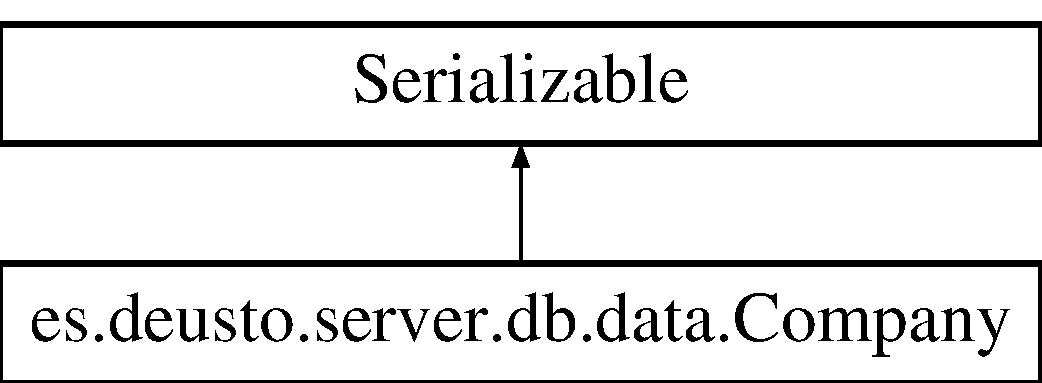
\includegraphics[height=2.000000cm]{classes_1_1deusto_1_1server_1_1db_1_1data_1_1_company}
\end{center}
\end{figure}
\subsection*{Public Member Functions}
\begin{DoxyCompactItemize}
\item 
\hyperlink{classes_1_1deusto_1_1server_1_1db_1_1data_1_1_company_acdee89103d4e157b7d4016fd8cd26d5e}{Company} (String \hyperlink{classes_1_1deusto_1_1server_1_1db_1_1data_1_1_company_a3080458c34b5cf83c7f8e866a93e60ac}{name})
\item 
void \hyperlink{classes_1_1deusto_1_1server_1_1db_1_1data_1_1_company_a99f3f91509e0a1ff5fc4d4d6a6219e77}{add\+Game} (\hyperlink{classes_1_1deusto_1_1server_1_1db_1_1data_1_1_game}{Game} game)
\item 
String \hyperlink{classes_1_1deusto_1_1server_1_1db_1_1data_1_1_company_a3bf0781fd4ec441406a5f8a05f293a23}{get\+Name} ()
\item 
String \hyperlink{classes_1_1deusto_1_1server_1_1db_1_1data_1_1_company_a3896b4f463ebed4f07fd3d9d0639b75a}{to\+String} ()
\end{DoxyCompactItemize}
\subsection*{Protected Attributes}
\begin{DoxyCompactItemize}
\item 
String \hyperlink{classes_1_1deusto_1_1server_1_1db_1_1data_1_1_company_a3080458c34b5cf83c7f8e866a93e60ac}{name} =null
\end{DoxyCompactItemize}


\subsection{Detailed Description}


Definition at line 33 of file Company.\+java.



\subsection{Constructor \& Destructor Documentation}
\mbox{\Hypertarget{classes_1_1deusto_1_1server_1_1db_1_1data_1_1_company_acdee89103d4e157b7d4016fd8cd26d5e}\label{classes_1_1deusto_1_1server_1_1db_1_1data_1_1_company_acdee89103d4e157b7d4016fd8cd26d5e}} 
\index{es\+::deusto\+::server\+::db\+::data\+::\+Company@{es\+::deusto\+::server\+::db\+::data\+::\+Company}!Company@{Company}}
\index{Company@{Company}!es\+::deusto\+::server\+::db\+::data\+::\+Company@{es\+::deusto\+::server\+::db\+::data\+::\+Company}}
\subsubsection{\texorpdfstring{Company()}{Company()}}
{\footnotesize\ttfamily es.\+deusto.\+server.\+db.\+data.\+Company.\+Company (\begin{DoxyParamCaption}\item[{String}]{name }\end{DoxyParamCaption})}



Definition at line 42 of file Company.\+java.



\subsection{Member Function Documentation}
\mbox{\Hypertarget{classes_1_1deusto_1_1server_1_1db_1_1data_1_1_company_a99f3f91509e0a1ff5fc4d4d6a6219e77}\label{classes_1_1deusto_1_1server_1_1db_1_1data_1_1_company_a99f3f91509e0a1ff5fc4d4d6a6219e77}} 
\index{es\+::deusto\+::server\+::db\+::data\+::\+Company@{es\+::deusto\+::server\+::db\+::data\+::\+Company}!add\+Game@{add\+Game}}
\index{add\+Game@{add\+Game}!es\+::deusto\+::server\+::db\+::data\+::\+Company@{es\+::deusto\+::server\+::db\+::data\+::\+Company}}
\subsubsection{\texorpdfstring{add\+Game()}{addGame()}}
{\footnotesize\ttfamily void es.\+deusto.\+server.\+db.\+data.\+Company.\+add\+Game (\begin{DoxyParamCaption}\item[{\hyperlink{classes_1_1deusto_1_1server_1_1db_1_1data_1_1_game}{Game}}]{game }\end{DoxyParamCaption})}



Definition at line 48 of file Company.\+java.

\mbox{\Hypertarget{classes_1_1deusto_1_1server_1_1db_1_1data_1_1_company_a3bf0781fd4ec441406a5f8a05f293a23}\label{classes_1_1deusto_1_1server_1_1db_1_1data_1_1_company_a3bf0781fd4ec441406a5f8a05f293a23}} 
\index{es\+::deusto\+::server\+::db\+::data\+::\+Company@{es\+::deusto\+::server\+::db\+::data\+::\+Company}!get\+Name@{get\+Name}}
\index{get\+Name@{get\+Name}!es\+::deusto\+::server\+::db\+::data\+::\+Company@{es\+::deusto\+::server\+::db\+::data\+::\+Company}}
\subsubsection{\texorpdfstring{get\+Name()}{getName()}}
{\footnotesize\ttfamily String es.\+deusto.\+server.\+db.\+data.\+Company.\+get\+Name (\begin{DoxyParamCaption}{ }\end{DoxyParamCaption})}



Definition at line 52 of file Company.\+java.

\mbox{\Hypertarget{classes_1_1deusto_1_1server_1_1db_1_1data_1_1_company_a3896b4f463ebed4f07fd3d9d0639b75a}\label{classes_1_1deusto_1_1server_1_1db_1_1data_1_1_company_a3896b4f463ebed4f07fd3d9d0639b75a}} 
\index{es\+::deusto\+::server\+::db\+::data\+::\+Company@{es\+::deusto\+::server\+::db\+::data\+::\+Company}!to\+String@{to\+String}}
\index{to\+String@{to\+String}!es\+::deusto\+::server\+::db\+::data\+::\+Company@{es\+::deusto\+::server\+::db\+::data\+::\+Company}}
\subsubsection{\texorpdfstring{to\+String()}{toString()}}
{\footnotesize\ttfamily String es.\+deusto.\+server.\+db.\+data.\+Company.\+to\+String (\begin{DoxyParamCaption}{ }\end{DoxyParamCaption})}



Definition at line 57 of file Company.\+java.



\subsection{Member Data Documentation}
\mbox{\Hypertarget{classes_1_1deusto_1_1server_1_1db_1_1data_1_1_company_a3080458c34b5cf83c7f8e866a93e60ac}\label{classes_1_1deusto_1_1server_1_1db_1_1data_1_1_company_a3080458c34b5cf83c7f8e866a93e60ac}} 
\index{es\+::deusto\+::server\+::db\+::data\+::\+Company@{es\+::deusto\+::server\+::db\+::data\+::\+Company}!name@{name}}
\index{name@{name}!es\+::deusto\+::server\+::db\+::data\+::\+Company@{es\+::deusto\+::server\+::db\+::data\+::\+Company}}
\subsubsection{\texorpdfstring{name}{name}}
{\footnotesize\ttfamily String es.\+deusto.\+server.\+db.\+data.\+Company.\+name =null\hspace{0.3cm}{\ttfamily [protected]}}



Definition at line 37 of file Company.\+java.



The documentation for this class was generated from the following file\+:\begin{DoxyCompactItemize}
\item 
src/main/java/es/deusto/server/db/data/\hyperlink{_company_8java}{Company.\+java}\end{DoxyCompactItemize}

\hypertarget{classes_1_1deusto_1_1server_1_1_conti_perf_test}{}\section{es.\+deusto.\+server.\+Conti\+Perf\+Test Class Reference}
\label{classes_1_1deusto_1_1server_1_1_conti_perf_test}\index{es.\+deusto.\+server.\+Conti\+Perf\+Test@{es.\+deusto.\+server.\+Conti\+Perf\+Test}}
\subsection*{Public Member Functions}
\begin{DoxyCompactItemize}
\item 
void \hyperlink{classes_1_1deusto_1_1server_1_1_conti_perf_test_ae0b0bd4dc05c61facbe80fac922ecdfa}{store\+Game\+Invocation\+Fail} ()
\item 
void \hyperlink{classes_1_1deusto_1_1server_1_1_conti_perf_test_a9d54db7715e9086710eb3c68b21b1013}{store\+Game\+Duration} ()
\item 
void \hyperlink{classes_1_1deusto_1_1server_1_1_conti_perf_test_aa7b6dc37eb9e76dd62e4f9040f7f7da9}{load\+Game} ()
\item 
void \hyperlink{classes_1_1deusto_1_1server_1_1_conti_perf_test_a980b2db90ab40f9bc7c7ec6ec3fcac4d}{load\+Game2} ()
\end{DoxyCompactItemize}
\subsection*{Static Public Member Functions}
\begin{DoxyCompactItemize}
\item 
static junit.\+framework.\+Test \hyperlink{classes_1_1deusto_1_1server_1_1_conti_perf_test_abe1f2e0ee16352a969c96e46dd35d770}{suite} ()
\end{DoxyCompactItemize}
\subsection*{Public Attributes}
\begin{DoxyCompactItemize}
\item 
Conti\+Perf\+Rule \hyperlink{classes_1_1deusto_1_1server_1_1_conti_perf_test_a36643de9d25126a2f4d24e6b61987c31}{rule} = new Conti\+Perf\+Rule()
\end{DoxyCompactItemize}


\subsection{Detailed Description}


Definition at line 52 of file Conti\+Perf\+Test.\+java.



\subsection{Member Function Documentation}
\mbox{\Hypertarget{classes_1_1deusto_1_1server_1_1_conti_perf_test_aa7b6dc37eb9e76dd62e4f9040f7f7da9}\label{classes_1_1deusto_1_1server_1_1_conti_perf_test_aa7b6dc37eb9e76dd62e4f9040f7f7da9}} 
\index{es\+::deusto\+::server\+::\+Conti\+Perf\+Test@{es\+::deusto\+::server\+::\+Conti\+Perf\+Test}!load\+Game@{load\+Game}}
\index{load\+Game@{load\+Game}!es\+::deusto\+::server\+::\+Conti\+Perf\+Test@{es\+::deusto\+::server\+::\+Conti\+Perf\+Test}}
\subsubsection{\texorpdfstring{load\+Game()}{loadGame()}}
{\footnotesize\ttfamily void es.\+deusto.\+server.\+Conti\+Perf\+Test.\+load\+Game (\begin{DoxyParamCaption}{ }\end{DoxyParamCaption})}



Definition at line 118 of file Conti\+Perf\+Test.\+java.

\mbox{\Hypertarget{classes_1_1deusto_1_1server_1_1_conti_perf_test_a980b2db90ab40f9bc7c7ec6ec3fcac4d}\label{classes_1_1deusto_1_1server_1_1_conti_perf_test_a980b2db90ab40f9bc7c7ec6ec3fcac4d}} 
\index{es\+::deusto\+::server\+::\+Conti\+Perf\+Test@{es\+::deusto\+::server\+::\+Conti\+Perf\+Test}!load\+Game2@{load\+Game2}}
\index{load\+Game2@{load\+Game2}!es\+::deusto\+::server\+::\+Conti\+Perf\+Test@{es\+::deusto\+::server\+::\+Conti\+Perf\+Test}}
\subsubsection{\texorpdfstring{load\+Game2()}{loadGame2()}}
{\footnotesize\ttfamily void es.\+deusto.\+server.\+Conti\+Perf\+Test.\+load\+Game2 (\begin{DoxyParamCaption}{ }\end{DoxyParamCaption})}



Definition at line 126 of file Conti\+Perf\+Test.\+java.

\mbox{\Hypertarget{classes_1_1deusto_1_1server_1_1_conti_perf_test_a9d54db7715e9086710eb3c68b21b1013}\label{classes_1_1deusto_1_1server_1_1_conti_perf_test_a9d54db7715e9086710eb3c68b21b1013}} 
\index{es\+::deusto\+::server\+::\+Conti\+Perf\+Test@{es\+::deusto\+::server\+::\+Conti\+Perf\+Test}!store\+Game\+Duration@{store\+Game\+Duration}}
\index{store\+Game\+Duration@{store\+Game\+Duration}!es\+::deusto\+::server\+::\+Conti\+Perf\+Test@{es\+::deusto\+::server\+::\+Conti\+Perf\+Test}}
\subsubsection{\texorpdfstring{store\+Game\+Duration()}{storeGameDuration()}}
{\footnotesize\ttfamily void es.\+deusto.\+server.\+Conti\+Perf\+Test.\+store\+Game\+Duration (\begin{DoxyParamCaption}{ }\end{DoxyParamCaption})}



Definition at line 103 of file Conti\+Perf\+Test.\+java.

\mbox{\Hypertarget{classes_1_1deusto_1_1server_1_1_conti_perf_test_ae0b0bd4dc05c61facbe80fac922ecdfa}\label{classes_1_1deusto_1_1server_1_1_conti_perf_test_ae0b0bd4dc05c61facbe80fac922ecdfa}} 
\index{es\+::deusto\+::server\+::\+Conti\+Perf\+Test@{es\+::deusto\+::server\+::\+Conti\+Perf\+Test}!store\+Game\+Invocation\+Fail@{store\+Game\+Invocation\+Fail}}
\index{store\+Game\+Invocation\+Fail@{store\+Game\+Invocation\+Fail}!es\+::deusto\+::server\+::\+Conti\+Perf\+Test@{es\+::deusto\+::server\+::\+Conti\+Perf\+Test}}
\subsubsection{\texorpdfstring{store\+Game\+Invocation\+Fail()}{storeGameInvocationFail()}}
{\footnotesize\ttfamily void es.\+deusto.\+server.\+Conti\+Perf\+Test.\+store\+Game\+Invocation\+Fail (\begin{DoxyParamCaption}{ }\end{DoxyParamCaption})}



Definition at line 77 of file Conti\+Perf\+Test.\+java.

\mbox{\Hypertarget{classes_1_1deusto_1_1server_1_1_conti_perf_test_abe1f2e0ee16352a969c96e46dd35d770}\label{classes_1_1deusto_1_1server_1_1_conti_perf_test_abe1f2e0ee16352a969c96e46dd35d770}} 
\index{es\+::deusto\+::server\+::\+Conti\+Perf\+Test@{es\+::deusto\+::server\+::\+Conti\+Perf\+Test}!suite@{suite}}
\index{suite@{suite}!es\+::deusto\+::server\+::\+Conti\+Perf\+Test@{es\+::deusto\+::server\+::\+Conti\+Perf\+Test}}
\subsubsection{\texorpdfstring{suite()}{suite()}}
{\footnotesize\ttfamily static junit.\+framework.\+Test es.\+deusto.\+server.\+Conti\+Perf\+Test.\+suite (\begin{DoxyParamCaption}{ }\end{DoxyParamCaption})\hspace{0.3cm}{\ttfamily [static]}}



Definition at line 68 of file Conti\+Perf\+Test.\+java.



\subsection{Member Data Documentation}
\mbox{\Hypertarget{classes_1_1deusto_1_1server_1_1_conti_perf_test_a36643de9d25126a2f4d24e6b61987c31}\label{classes_1_1deusto_1_1server_1_1_conti_perf_test_a36643de9d25126a2f4d24e6b61987c31}} 
\index{es\+::deusto\+::server\+::\+Conti\+Perf\+Test@{es\+::deusto\+::server\+::\+Conti\+Perf\+Test}!rule@{rule}}
\index{rule@{rule}!es\+::deusto\+::server\+::\+Conti\+Perf\+Test@{es\+::deusto\+::server\+::\+Conti\+Perf\+Test}}
\subsubsection{\texorpdfstring{rule}{rule}}
{\footnotesize\ttfamily Conti\+Perf\+Rule es.\+deusto.\+server.\+Conti\+Perf\+Test.\+rule = new Conti\+Perf\+Rule()}



Definition at line 66 of file Conti\+Perf\+Test.\+java.



The documentation for this class was generated from the following file\+:\begin{DoxyCompactItemize}
\item 
C\+:/\+Users/\+Marta/\+S\+P\+Q09/\+Lurrun/src/test/java/es/deusto/server/\hyperlink{_conti_perf_test_8java}{Conti\+Perf\+Test.\+java}\end{DoxyCompactItemize}

\hypertarget{classes_1_1deusto_1_1server_1_1db_1_1dao_1_1_d_a_o}{}\section{es.\+deusto.\+server.\+db.\+dao.\+D\+AO Class Reference}
\label{classes_1_1deusto_1_1server_1_1db_1_1dao_1_1_d_a_o}\index{es.\+deusto.\+server.\+db.\+dao.\+D\+AO@{es.\+deusto.\+server.\+db.\+dao.\+D\+AO}}
Inheritance diagram for es.\+deusto.\+server.\+db.\+dao.\+D\+AO\+:\begin{figure}[H]
\begin{center}
\leavevmode
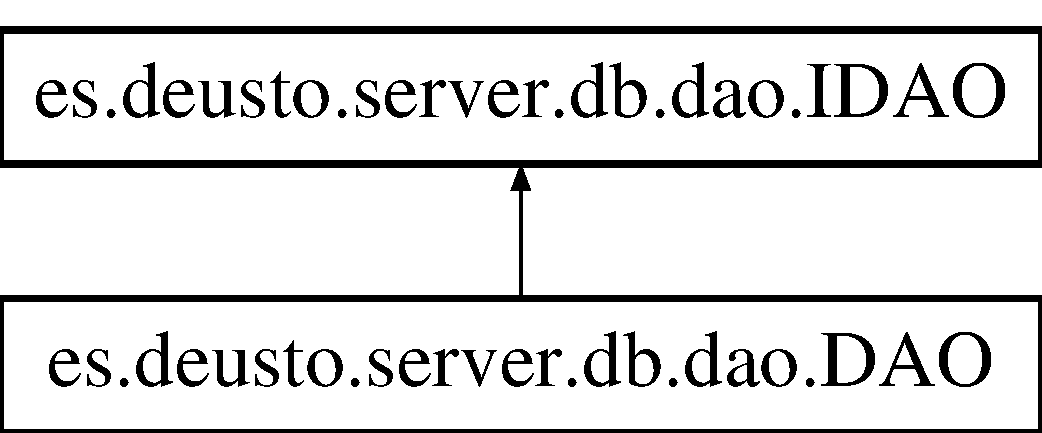
\includegraphics[height=2.000000cm]{classes_1_1deusto_1_1server_1_1db_1_1dao_1_1_d_a_o}
\end{center}
\end{figure}
\subsection*{Public Member Functions}
\begin{DoxyCompactItemize}
\item 
\hyperlink{classes_1_1deusto_1_1server_1_1db_1_1dao_1_1_d_a_o_a1f12a4ca454651d41896e45c42db8f90}{D\+AO} ()
\item 
boolean \hyperlink{classes_1_1deusto_1_1server_1_1db_1_1dao_1_1_d_a_o_acb146e96959c340ef828ef8e36b4283c}{store\+User} (\hyperlink{classes_1_1deusto_1_1server_1_1db_1_1data_1_1_user}{User} u)
\item 
boolean \hyperlink{classes_1_1deusto_1_1server_1_1db_1_1dao_1_1_d_a_o_a98774e8d93cdd4d8d104a197bd37d4e1}{update\+License} (\hyperlink{classes_1_1deusto_1_1server_1_1db_1_1data_1_1_license}{License} g)
\item 
\hyperlink{classes_1_1deusto_1_1server_1_1db_1_1data_1_1_user}{User} \hyperlink{classes_1_1deusto_1_1server_1_1db_1_1dao_1_1_d_a_o_a8c316b4c3bf246d00fb2b423a603ebe6}{retrieve\+User} (String login)
\item 
boolean \hyperlink{classes_1_1deusto_1_1server_1_1db_1_1dao_1_1_d_a_o_a7f6ed77294fe1f61cbebbea410cef6e0}{update\+User} (\hyperlink{classes_1_1deusto_1_1server_1_1db_1_1data_1_1_user}{User} u)
\item 
boolean \hyperlink{classes_1_1deusto_1_1server_1_1db_1_1dao_1_1_d_a_o_a7484309d9b9b39c24cd7d0413a90c468}{store\+Game} (\hyperlink{classes_1_1deusto_1_1server_1_1db_1_1data_1_1_game}{Game} g)
\item 
boolean \hyperlink{classes_1_1deusto_1_1server_1_1db_1_1dao_1_1_d_a_o_ae7540010b43f96c5e50995a8376614e7}{update\+Game} (\hyperlink{classes_1_1deusto_1_1server_1_1db_1_1data_1_1_game}{Game} g)
\item 
boolean \hyperlink{classes_1_1deusto_1_1server_1_1db_1_1dao_1_1_d_a_o_a0748467c3346a5bcdcd79b508562b6dc}{update\+Company} (\hyperlink{classes_1_1deusto_1_1server_1_1db_1_1data_1_1_company}{Company} c)
\item 
boolean \hyperlink{classes_1_1deusto_1_1server_1_1db_1_1dao_1_1_d_a_o_ae08384fb32fa6936c93f6292dbe02c7e}{update\+Genre} (\hyperlink{classes_1_1deusto_1_1server_1_1db_1_1data_1_1_genre}{Genre} g)
\item 
List$<$ \hyperlink{classes_1_1deusto_1_1server_1_1db_1_1data_1_1_game}{Game} $>$ \hyperlink{classes_1_1deusto_1_1server_1_1db_1_1dao_1_1_d_a_o_af49ed57bdac4dec48ab7616602d12df2}{get\+All\+Games} ()
\item 
List$<$ \hyperlink{classes_1_1deusto_1_1server_1_1db_1_1data_1_1_company}{Company} $>$ \hyperlink{classes_1_1deusto_1_1server_1_1db_1_1dao_1_1_d_a_o_ac564970c7e308393497e874655470aaa}{get\+All\+Companies} ()
\item 
List$<$ \hyperlink{classes_1_1deusto_1_1server_1_1db_1_1data_1_1_genre}{Genre} $>$ \hyperlink{classes_1_1deusto_1_1server_1_1db_1_1dao_1_1_d_a_o_ac1cb7032ef21f53dead8347ef440f431}{get\+All\+Genres} ()
\item 
List$<$ \hyperlink{classes_1_1deusto_1_1server_1_1db_1_1data_1_1_user}{User} $>$ \hyperlink{classes_1_1deusto_1_1server_1_1db_1_1dao_1_1_d_a_o_a9c59f6c4bf89f46e305f88a4f8eb96bc}{get\+All\+Users} ()
\item 
\hyperlink{classes_1_1deusto_1_1server_1_1db_1_1data_1_1_license}{License} \hyperlink{classes_1_1deusto_1_1server_1_1db_1_1dao_1_1_d_a_o_a4a5a54059bac00ea6f3b6d21f2a31a02}{get\+First\+License} (String name)
\item 
\hyperlink{classes_1_1deusto_1_1server_1_1db_1_1data_1_1_genre}{Genre} \hyperlink{classes_1_1deusto_1_1server_1_1db_1_1dao_1_1_d_a_o_a16b0af798fbb00cd29a505491c57e2cd}{retrieve\+Genre} (String name)
\item 
\hyperlink{classes_1_1deusto_1_1server_1_1db_1_1data_1_1_game}{Game} \hyperlink{classes_1_1deusto_1_1server_1_1db_1_1dao_1_1_d_a_o_ac94a91d3e5aeeb98fc12f087532b3506}{retrieve\+Game} (String name)
\item 
\hyperlink{classes_1_1deusto_1_1server_1_1db_1_1data_1_1_company}{Company} \hyperlink{classes_1_1deusto_1_1server_1_1db_1_1dao_1_1_d_a_o_aabd374b169473cfd6e1bdc4efc89b177}{retrieve\+Company} (String name)
\item 
\hyperlink{classes_1_1deusto_1_1server_1_1db_1_1data_1_1_license}{License} \hyperlink{classes_1_1deusto_1_1server_1_1db_1_1dao_1_1_d_a_o_a02fd634e6bd7a087b1476ab161af646f}{retrieve\+License} (String game\+Key)
\end{DoxyCompactItemize}


\subsection{Detailed Description}
This class is the link between the database and the server \begin{DoxyAuthor}{Author}

\end{DoxyAuthor}
\begin{DoxyVersion}{Version}
1.\+0 
\end{DoxyVersion}
\begin{DoxySince}{Since}
24/03/2017 
\end{DoxySince}


Definition at line 22 of file D\+A\+O.\+java.



\subsection{Constructor \& Destructor Documentation}
\mbox{\Hypertarget{classes_1_1deusto_1_1server_1_1db_1_1dao_1_1_d_a_o_a1f12a4ca454651d41896e45c42db8f90}\label{classes_1_1deusto_1_1server_1_1db_1_1dao_1_1_d_a_o_a1f12a4ca454651d41896e45c42db8f90}} 
\index{es\+::deusto\+::server\+::db\+::dao\+::\+D\+AO@{es\+::deusto\+::server\+::db\+::dao\+::\+D\+AO}!D\+AO@{D\+AO}}
\index{D\+AO@{D\+AO}!es\+::deusto\+::server\+::db\+::dao\+::\+D\+AO@{es\+::deusto\+::server\+::db\+::dao\+::\+D\+AO}}
\subsubsection{\texorpdfstring{D\+A\+O()}{DAO()}}
{\footnotesize\ttfamily es.\+deusto.\+server.\+db.\+dao.\+D\+A\+O.\+D\+AO (\begin{DoxyParamCaption}{ }\end{DoxyParamCaption})}



Definition at line 27 of file D\+A\+O.\+java.



\subsection{Member Function Documentation}
\mbox{\Hypertarget{classes_1_1deusto_1_1server_1_1db_1_1dao_1_1_d_a_o_ac564970c7e308393497e874655470aaa}\label{classes_1_1deusto_1_1server_1_1db_1_1dao_1_1_d_a_o_ac564970c7e308393497e874655470aaa}} 
\index{es\+::deusto\+::server\+::db\+::dao\+::\+D\+AO@{es\+::deusto\+::server\+::db\+::dao\+::\+D\+AO}!get\+All\+Companies@{get\+All\+Companies}}
\index{get\+All\+Companies@{get\+All\+Companies}!es\+::deusto\+::server\+::db\+::dao\+::\+D\+AO@{es\+::deusto\+::server\+::db\+::dao\+::\+D\+AO}}
\subsubsection{\texorpdfstring{get\+All\+Companies()}{getAllCompanies()}}
{\footnotesize\ttfamily List$<$\hyperlink{classes_1_1deusto_1_1server_1_1db_1_1data_1_1_company}{Company}$>$ es.\+deusto.\+server.\+db.\+dao.\+D\+A\+O.\+get\+All\+Companies (\begin{DoxyParamCaption}{ }\end{DoxyParamCaption})}

This method shows all the companies 
\begin{DoxyParams}{Parameters}
{\em unused} & \\
\hline
\end{DoxyParams}
\begin{DoxyReturn}{Returns}
List Returns a list of companies 
\end{DoxyReturn}
\begin{DoxySeeAlso}{See also}
\hyperlink{interfacees_1_1deusto_1_1server_1_1db_1_1dao_1_1_i_d_a_o_ad83c37658f356cb69c1fa70f99416579}{es.\+deusto.\+server.\+db.\+dao.\+I\+D\+A\+O\+::get\+All\+Companies()} 
\end{DoxySeeAlso}


Implements \hyperlink{interfacees_1_1deusto_1_1server_1_1db_1_1dao_1_1_i_d_a_o_ad83c37658f356cb69c1fa70f99416579}{es.\+deusto.\+server.\+db.\+dao.\+I\+D\+AO}.



Definition at line 415 of file D\+A\+O.\+java.

\mbox{\Hypertarget{classes_1_1deusto_1_1server_1_1db_1_1dao_1_1_d_a_o_af49ed57bdac4dec48ab7616602d12df2}\label{classes_1_1deusto_1_1server_1_1db_1_1dao_1_1_d_a_o_af49ed57bdac4dec48ab7616602d12df2}} 
\index{es\+::deusto\+::server\+::db\+::dao\+::\+D\+AO@{es\+::deusto\+::server\+::db\+::dao\+::\+D\+AO}!get\+All\+Games@{get\+All\+Games}}
\index{get\+All\+Games@{get\+All\+Games}!es\+::deusto\+::server\+::db\+::dao\+::\+D\+AO@{es\+::deusto\+::server\+::db\+::dao\+::\+D\+AO}}
\subsubsection{\texorpdfstring{get\+All\+Games()}{getAllGames()}}
{\footnotesize\ttfamily List$<$\hyperlink{classes_1_1deusto_1_1server_1_1db_1_1data_1_1_game}{Game}$>$ es.\+deusto.\+server.\+db.\+dao.\+D\+A\+O.\+get\+All\+Games (\begin{DoxyParamCaption}{ }\end{DoxyParamCaption})}

This method shows a list of games 
\begin{DoxyParams}{Parameters}
{\em unused} & \\
\hline
\end{DoxyParams}
\begin{DoxyReturn}{Returns}
List Returns a list of games 
\end{DoxyReturn}
\begin{DoxySeeAlso}{See also}
\hyperlink{interfacees_1_1deusto_1_1server_1_1db_1_1dao_1_1_i_d_a_o_aebafef372cf3064b12d16fcb651b41ff}{es.\+deusto.\+server.\+db.\+dao.\+I\+D\+A\+O\+::get\+All\+Games()} 
\end{DoxySeeAlso}


Implements \hyperlink{interfacees_1_1deusto_1_1server_1_1db_1_1dao_1_1_i_d_a_o_aebafef372cf3064b12d16fcb651b41ff}{es.\+deusto.\+server.\+db.\+dao.\+I\+D\+AO}.



Definition at line 377 of file D\+A\+O.\+java.

\mbox{\Hypertarget{classes_1_1deusto_1_1server_1_1db_1_1dao_1_1_d_a_o_ac1cb7032ef21f53dead8347ef440f431}\label{classes_1_1deusto_1_1server_1_1db_1_1dao_1_1_d_a_o_ac1cb7032ef21f53dead8347ef440f431}} 
\index{es\+::deusto\+::server\+::db\+::dao\+::\+D\+AO@{es\+::deusto\+::server\+::db\+::dao\+::\+D\+AO}!get\+All\+Genres@{get\+All\+Genres}}
\index{get\+All\+Genres@{get\+All\+Genres}!es\+::deusto\+::server\+::db\+::dao\+::\+D\+AO@{es\+::deusto\+::server\+::db\+::dao\+::\+D\+AO}}
\subsubsection{\texorpdfstring{get\+All\+Genres()}{getAllGenres()}}
{\footnotesize\ttfamily List$<$\hyperlink{classes_1_1deusto_1_1server_1_1db_1_1data_1_1_genre}{Genre}$>$ es.\+deusto.\+server.\+db.\+dao.\+D\+A\+O.\+get\+All\+Genres (\begin{DoxyParamCaption}{ }\end{DoxyParamCaption})}

This method shows all the genres 
\begin{DoxyParams}{Parameters}
{\em unused} & \\
\hline
\end{DoxyParams}
\begin{DoxyReturn}{Returns}
List Returns a list of genres 
\end{DoxyReturn}
\begin{DoxySeeAlso}{See also}
\hyperlink{interfacees_1_1deusto_1_1server_1_1db_1_1dao_1_1_i_d_a_o_a96ad8de066318847a7828b12befe94f7}{es.\+deusto.\+server.\+db.\+dao.\+I\+D\+A\+O\+::get\+All\+Genres()} 
\end{DoxySeeAlso}


Implements \hyperlink{interfacees_1_1deusto_1_1server_1_1db_1_1dao_1_1_i_d_a_o_a96ad8de066318847a7828b12befe94f7}{es.\+deusto.\+server.\+db.\+dao.\+I\+D\+AO}.



Definition at line 452 of file D\+A\+O.\+java.

\mbox{\Hypertarget{classes_1_1deusto_1_1server_1_1db_1_1dao_1_1_d_a_o_a9c59f6c4bf89f46e305f88a4f8eb96bc}\label{classes_1_1deusto_1_1server_1_1db_1_1dao_1_1_d_a_o_a9c59f6c4bf89f46e305f88a4f8eb96bc}} 
\index{es\+::deusto\+::server\+::db\+::dao\+::\+D\+AO@{es\+::deusto\+::server\+::db\+::dao\+::\+D\+AO}!get\+All\+Users@{get\+All\+Users}}
\index{get\+All\+Users@{get\+All\+Users}!es\+::deusto\+::server\+::db\+::dao\+::\+D\+AO@{es\+::deusto\+::server\+::db\+::dao\+::\+D\+AO}}
\subsubsection{\texorpdfstring{get\+All\+Users()}{getAllUsers()}}
{\footnotesize\ttfamily List$<$\hyperlink{classes_1_1deusto_1_1server_1_1db_1_1data_1_1_user}{User}$>$ es.\+deusto.\+server.\+db.\+dao.\+D\+A\+O.\+get\+All\+Users (\begin{DoxyParamCaption}{ }\end{DoxyParamCaption})}

This method shows a list of users 
\begin{DoxyParams}{Parameters}
{\em unused} & \\
\hline
\end{DoxyParams}
\begin{DoxyReturn}{Returns}
List Returns a list of users 
\end{DoxyReturn}
\begin{DoxySeeAlso}{See also}
es.\+deusto.\+server.\+db.\+dao.\+I\+D\+A\+O\+::get\+All\+Users() 
\end{DoxySeeAlso}


Definition at line 488 of file D\+A\+O.\+java.

\mbox{\Hypertarget{classes_1_1deusto_1_1server_1_1db_1_1dao_1_1_d_a_o_a4a5a54059bac00ea6f3b6d21f2a31a02}\label{classes_1_1deusto_1_1server_1_1db_1_1dao_1_1_d_a_o_a4a5a54059bac00ea6f3b6d21f2a31a02}} 
\index{es\+::deusto\+::server\+::db\+::dao\+::\+D\+AO@{es\+::deusto\+::server\+::db\+::dao\+::\+D\+AO}!get\+First\+License@{get\+First\+License}}
\index{get\+First\+License@{get\+First\+License}!es\+::deusto\+::server\+::db\+::dao\+::\+D\+AO@{es\+::deusto\+::server\+::db\+::dao\+::\+D\+AO}}
\subsubsection{\texorpdfstring{get\+First\+License()}{getFirstLicense()}}
{\footnotesize\ttfamily \hyperlink{classes_1_1deusto_1_1server_1_1db_1_1data_1_1_license}{License} es.\+deusto.\+server.\+db.\+dao.\+D\+A\+O.\+get\+First\+License (\begin{DoxyParamCaption}\item[{String}]{name }\end{DoxyParamCaption})}

This method returns the first license stored in the database 
\begin{DoxyParams}{Parameters}
{\em name} & This is the name of a license \\
\hline
\end{DoxyParams}
\begin{DoxyReturn}{Returns}
License Returns a license 
\end{DoxyReturn}
\begin{DoxySeeAlso}{See also}
\hyperlink{interfacees_1_1deusto_1_1server_1_1db_1_1dao_1_1_i_d_a_o_aef2783889a572e23bd57c5a2a955599a}{es.\+deusto.\+server.\+db.\+dao.\+I\+D\+A\+O\+::get\+First\+License}(java.\+lang.\+String) 
\end{DoxySeeAlso}


Implements \hyperlink{interfacees_1_1deusto_1_1server_1_1db_1_1dao_1_1_i_d_a_o_aef2783889a572e23bd57c5a2a955599a}{es.\+deusto.\+server.\+db.\+dao.\+I\+D\+AO}.



Definition at line 527 of file D\+A\+O.\+java.

\mbox{\Hypertarget{classes_1_1deusto_1_1server_1_1db_1_1dao_1_1_d_a_o_aabd374b169473cfd6e1bdc4efc89b177}\label{classes_1_1deusto_1_1server_1_1db_1_1dao_1_1_d_a_o_aabd374b169473cfd6e1bdc4efc89b177}} 
\index{es\+::deusto\+::server\+::db\+::dao\+::\+D\+AO@{es\+::deusto\+::server\+::db\+::dao\+::\+D\+AO}!retrieve\+Company@{retrieve\+Company}}
\index{retrieve\+Company@{retrieve\+Company}!es\+::deusto\+::server\+::db\+::dao\+::\+D\+AO@{es\+::deusto\+::server\+::db\+::dao\+::\+D\+AO}}
\subsubsection{\texorpdfstring{retrieve\+Company()}{retrieveCompany()}}
{\footnotesize\ttfamily \hyperlink{classes_1_1deusto_1_1server_1_1db_1_1data_1_1_company}{Company} es.\+deusto.\+server.\+db.\+dao.\+D\+A\+O.\+retrieve\+Company (\begin{DoxyParamCaption}\item[{String}]{name }\end{DoxyParamCaption})}

This method retrieves a company 
\begin{DoxyParams}{Parameters}
{\em name} & This is the name of a company \\
\hline
\end{DoxyParams}
\begin{DoxyReturn}{Returns}
Company Returns a company 
\end{DoxyReturn}
\begin{DoxySeeAlso}{See also}
\hyperlink{interfacees_1_1deusto_1_1server_1_1db_1_1dao_1_1_i_d_a_o_ad6fd7873e2191e887184e2261e34e3e5}{es.\+deusto.\+server.\+db.\+dao.\+I\+D\+A\+O\+::retrieve\+Company}(java.\+lang.\+String) 
\end{DoxySeeAlso}


Implements \hyperlink{interfacees_1_1deusto_1_1server_1_1db_1_1dao_1_1_i_d_a_o_ad6fd7873e2191e887184e2261e34e3e5}{es.\+deusto.\+server.\+db.\+dao.\+I\+D\+AO}.



Definition at line 627 of file D\+A\+O.\+java.

\mbox{\Hypertarget{classes_1_1deusto_1_1server_1_1db_1_1dao_1_1_d_a_o_ac94a91d3e5aeeb98fc12f087532b3506}\label{classes_1_1deusto_1_1server_1_1db_1_1dao_1_1_d_a_o_ac94a91d3e5aeeb98fc12f087532b3506}} 
\index{es\+::deusto\+::server\+::db\+::dao\+::\+D\+AO@{es\+::deusto\+::server\+::db\+::dao\+::\+D\+AO}!retrieve\+Game@{retrieve\+Game}}
\index{retrieve\+Game@{retrieve\+Game}!es\+::deusto\+::server\+::db\+::dao\+::\+D\+AO@{es\+::deusto\+::server\+::db\+::dao\+::\+D\+AO}}
\subsubsection{\texorpdfstring{retrieve\+Game()}{retrieveGame()}}
{\footnotesize\ttfamily \hyperlink{classes_1_1deusto_1_1server_1_1db_1_1data_1_1_game}{Game} es.\+deusto.\+server.\+db.\+dao.\+D\+A\+O.\+retrieve\+Game (\begin{DoxyParamCaption}\item[{String}]{name }\end{DoxyParamCaption})}

This method retrieves a game 
\begin{DoxyParams}{Parameters}
{\em name} & This is the name of a game \\
\hline
\end{DoxyParams}
\begin{DoxyReturn}{Returns}
Game Returns a game 
\end{DoxyReturn}
\begin{DoxySeeAlso}{See also}
\hyperlink{interfacees_1_1deusto_1_1server_1_1db_1_1dao_1_1_i_d_a_o_a30558c19c086ac0ffff6796a8ae208fb}{es.\+deusto.\+server.\+db.\+dao.\+I\+D\+A\+O\+::retrieve\+Game}(java.\+lang.\+String) 
\end{DoxySeeAlso}


Implements \hyperlink{interfacees_1_1deusto_1_1server_1_1db_1_1dao_1_1_i_d_a_o_a30558c19c086ac0ffff6796a8ae208fb}{es.\+deusto.\+server.\+db.\+dao.\+I\+D\+AO}.



Definition at line 596 of file D\+A\+O.\+java.

\mbox{\Hypertarget{classes_1_1deusto_1_1server_1_1db_1_1dao_1_1_d_a_o_a16b0af798fbb00cd29a505491c57e2cd}\label{classes_1_1deusto_1_1server_1_1db_1_1dao_1_1_d_a_o_a16b0af798fbb00cd29a505491c57e2cd}} 
\index{es\+::deusto\+::server\+::db\+::dao\+::\+D\+AO@{es\+::deusto\+::server\+::db\+::dao\+::\+D\+AO}!retrieve\+Genre@{retrieve\+Genre}}
\index{retrieve\+Genre@{retrieve\+Genre}!es\+::deusto\+::server\+::db\+::dao\+::\+D\+AO@{es\+::deusto\+::server\+::db\+::dao\+::\+D\+AO}}
\subsubsection{\texorpdfstring{retrieve\+Genre()}{retrieveGenre()}}
{\footnotesize\ttfamily \hyperlink{classes_1_1deusto_1_1server_1_1db_1_1data_1_1_genre}{Genre} es.\+deusto.\+server.\+db.\+dao.\+D\+A\+O.\+retrieve\+Genre (\begin{DoxyParamCaption}\item[{String}]{name }\end{DoxyParamCaption})}

This methos retrieves a genre 
\begin{DoxyParams}{Parameters}
{\em name} & This is the name of a genre \\
\hline
\end{DoxyParams}
\begin{DoxyReturn}{Returns}
Genre Returns a genre 
\end{DoxyReturn}
\begin{DoxySeeAlso}{See also}
\hyperlink{interfacees_1_1deusto_1_1server_1_1db_1_1dao_1_1_i_d_a_o_a8b15955637f9b81c57900761c6d03571}{es.\+deusto.\+server.\+db.\+dao.\+I\+D\+A\+O\+::retrieve\+Genre}(java.\+lang.\+String) 
\end{DoxySeeAlso}


Implements \hyperlink{interfacees_1_1deusto_1_1server_1_1db_1_1dao_1_1_i_d_a_o_a8b15955637f9b81c57900761c6d03571}{es.\+deusto.\+server.\+db.\+dao.\+I\+D\+AO}.



Definition at line 565 of file D\+A\+O.\+java.

\mbox{\Hypertarget{classes_1_1deusto_1_1server_1_1db_1_1dao_1_1_d_a_o_a02fd634e6bd7a087b1476ab161af646f}\label{classes_1_1deusto_1_1server_1_1db_1_1dao_1_1_d_a_o_a02fd634e6bd7a087b1476ab161af646f}} 
\index{es\+::deusto\+::server\+::db\+::dao\+::\+D\+AO@{es\+::deusto\+::server\+::db\+::dao\+::\+D\+AO}!retrieve\+License@{retrieve\+License}}
\index{retrieve\+License@{retrieve\+License}!es\+::deusto\+::server\+::db\+::dao\+::\+D\+AO@{es\+::deusto\+::server\+::db\+::dao\+::\+D\+AO}}
\subsubsection{\texorpdfstring{retrieve\+License()}{retrieveLicense()}}
{\footnotesize\ttfamily \hyperlink{classes_1_1deusto_1_1server_1_1db_1_1data_1_1_license}{License} es.\+deusto.\+server.\+db.\+dao.\+D\+A\+O.\+retrieve\+License (\begin{DoxyParamCaption}\item[{String}]{game\+Key }\end{DoxyParamCaption})}

This method retrieves a license 
\begin{DoxyParams}{Parameters}
{\em game\+Key} & This is the key of a license \\
\hline
\end{DoxyParams}
\begin{DoxyReturn}{Returns}
License Returns a license 
\end{DoxyReturn}
\begin{DoxySeeAlso}{See also}
\hyperlink{interfacees_1_1deusto_1_1server_1_1db_1_1dao_1_1_i_d_a_o_a6a3e25055d4a81c738d1bd73de6ef7da}{es.\+deusto.\+server.\+db.\+dao.\+I\+D\+A\+O\+::retrieve\+License}(java.\+lang.\+String) 
\end{DoxySeeAlso}


Implements \hyperlink{interfacees_1_1deusto_1_1server_1_1db_1_1dao_1_1_i_d_a_o_a6a3e25055d4a81c738d1bd73de6ef7da}{es.\+deusto.\+server.\+db.\+dao.\+I\+D\+AO}.



Definition at line 658 of file D\+A\+O.\+java.

\mbox{\Hypertarget{classes_1_1deusto_1_1server_1_1db_1_1dao_1_1_d_a_o_a8c316b4c3bf246d00fb2b423a603ebe6}\label{classes_1_1deusto_1_1server_1_1db_1_1dao_1_1_d_a_o_a8c316b4c3bf246d00fb2b423a603ebe6}} 
\index{es\+::deusto\+::server\+::db\+::dao\+::\+D\+AO@{es\+::deusto\+::server\+::db\+::dao\+::\+D\+AO}!retrieve\+User@{retrieve\+User}}
\index{retrieve\+User@{retrieve\+User}!es\+::deusto\+::server\+::db\+::dao\+::\+D\+AO@{es\+::deusto\+::server\+::db\+::dao\+::\+D\+AO}}
\subsubsection{\texorpdfstring{retrieve\+User()}{retrieveUser()}}
{\footnotesize\ttfamily \hyperlink{classes_1_1deusto_1_1server_1_1db_1_1data_1_1_user}{User} es.\+deusto.\+server.\+db.\+dao.\+D\+A\+O.\+retrieve\+User (\begin{DoxyParamCaption}\item[{String}]{login }\end{DoxyParamCaption})}

This method retrieves a user 
\begin{DoxyParams}{Parameters}
{\em login} & This is the login name of a user \\
\hline
\end{DoxyParams}
\begin{DoxyReturn}{Returns}
User Returns a user 
\end{DoxyReturn}
\begin{DoxySeeAlso}{See also}
\hyperlink{interfacees_1_1deusto_1_1server_1_1db_1_1dao_1_1_i_d_a_o_a19f9b0d0b6f5f80730d6d197deca7dfc}{es.\+deusto.\+server.\+db.\+dao.\+I\+D\+A\+O\+::retrieve\+User}(java.\+lang.\+String) 
\end{DoxySeeAlso}


Implements \hyperlink{interfacees_1_1deusto_1_1server_1_1db_1_1dao_1_1_i_d_a_o_a19f9b0d0b6f5f80730d6d197deca7dfc}{es.\+deusto.\+server.\+db.\+dao.\+I\+D\+AO}.



Definition at line 98 of file D\+A\+O.\+java.

\mbox{\Hypertarget{classes_1_1deusto_1_1server_1_1db_1_1dao_1_1_d_a_o_a7484309d9b9b39c24cd7d0413a90c468}\label{classes_1_1deusto_1_1server_1_1db_1_1dao_1_1_d_a_o_a7484309d9b9b39c24cd7d0413a90c468}} 
\index{es\+::deusto\+::server\+::db\+::dao\+::\+D\+AO@{es\+::deusto\+::server\+::db\+::dao\+::\+D\+AO}!store\+Game@{store\+Game}}
\index{store\+Game@{store\+Game}!es\+::deusto\+::server\+::db\+::dao\+::\+D\+AO@{es\+::deusto\+::server\+::db\+::dao\+::\+D\+AO}}
\subsubsection{\texorpdfstring{store\+Game()}{storeGame()}}
{\footnotesize\ttfamily boolean es.\+deusto.\+server.\+db.\+dao.\+D\+A\+O.\+store\+Game (\begin{DoxyParamCaption}\item[{\hyperlink{classes_1_1deusto_1_1server_1_1db_1_1data_1_1_game}{Game}}]{g }\end{DoxyParamCaption})}

This method stores a game 
\begin{DoxyParams}{Parameters}
{\em g} & This is a game \\
\hline
\end{DoxyParams}
\begin{DoxyReturn}{Returns}
boolean Returns true or false depending on whether the game exists or not 
\end{DoxyReturn}
\begin{DoxySeeAlso}{See also}
\hyperlink{interfacees_1_1deusto_1_1server_1_1db_1_1dao_1_1_i_d_a_o_ab38972c7c70c95b4c409fa7758ef2fc3}{es.\+deusto.\+server.\+db.\+dao.\+I\+D\+A\+O\+::store\+Game}(\hyperlink{classes_1_1deusto_1_1server_1_1db_1_1data_1_1_game}{es.\+deusto.\+server.\+db.\+data.\+Game}) 
\end{DoxySeeAlso}


Implements \hyperlink{interfacees_1_1deusto_1_1server_1_1db_1_1dao_1_1_i_d_a_o_ab38972c7c70c95b4c409fa7758ef2fc3}{es.\+deusto.\+server.\+db.\+dao.\+I\+D\+AO}.



Definition at line 157 of file D\+A\+O.\+java.

\mbox{\Hypertarget{classes_1_1deusto_1_1server_1_1db_1_1dao_1_1_d_a_o_acb146e96959c340ef828ef8e36b4283c}\label{classes_1_1deusto_1_1server_1_1db_1_1dao_1_1_d_a_o_acb146e96959c340ef828ef8e36b4283c}} 
\index{es\+::deusto\+::server\+::db\+::dao\+::\+D\+AO@{es\+::deusto\+::server\+::db\+::dao\+::\+D\+AO}!store\+User@{store\+User}}
\index{store\+User@{store\+User}!es\+::deusto\+::server\+::db\+::dao\+::\+D\+AO@{es\+::deusto\+::server\+::db\+::dao\+::\+D\+AO}}
\subsubsection{\texorpdfstring{store\+User()}{storeUser()}}
{\footnotesize\ttfamily boolean es.\+deusto.\+server.\+db.\+dao.\+D\+A\+O.\+store\+User (\begin{DoxyParamCaption}\item[{\hyperlink{classes_1_1deusto_1_1server_1_1db_1_1data_1_1_user}{User}}]{u }\end{DoxyParamCaption})}

This method stores a user 
\begin{DoxyParams}{Parameters}
{\em u} & This is a user \\
\hline
\end{DoxyParams}
\begin{DoxyReturn}{Returns}
boolean Returns true or false depending on whether the user exists or not 
\end{DoxyReturn}
\begin{DoxySeeAlso}{See also}
\hyperlink{interfacees_1_1deusto_1_1server_1_1db_1_1dao_1_1_i_d_a_o_ab943216560f43595a852b406dcd394a4}{es.\+deusto.\+server.\+db.\+dao.\+I\+D\+A\+O\+::store\+User}(\hyperlink{classes_1_1deusto_1_1server_1_1db_1_1data_1_1_user}{es.\+deusto.\+server.\+db.\+data.\+User}) 
\end{DoxySeeAlso}


Implements \hyperlink{interfacees_1_1deusto_1_1server_1_1db_1_1dao_1_1_i_d_a_o_ab943216560f43595a852b406dcd394a4}{es.\+deusto.\+server.\+db.\+dao.\+I\+D\+AO}.



Definition at line 38 of file D\+A\+O.\+java.

\mbox{\Hypertarget{classes_1_1deusto_1_1server_1_1db_1_1dao_1_1_d_a_o_a0748467c3346a5bcdcd79b508562b6dc}\label{classes_1_1deusto_1_1server_1_1db_1_1dao_1_1_d_a_o_a0748467c3346a5bcdcd79b508562b6dc}} 
\index{es\+::deusto\+::server\+::db\+::dao\+::\+D\+AO@{es\+::deusto\+::server\+::db\+::dao\+::\+D\+AO}!update\+Company@{update\+Company}}
\index{update\+Company@{update\+Company}!es\+::deusto\+::server\+::db\+::dao\+::\+D\+AO@{es\+::deusto\+::server\+::db\+::dao\+::\+D\+AO}}
\subsubsection{\texorpdfstring{update\+Company()}{updateCompany()}}
{\footnotesize\ttfamily boolean es.\+deusto.\+server.\+db.\+dao.\+D\+A\+O.\+update\+Company (\begin{DoxyParamCaption}\item[{\hyperlink{classes_1_1deusto_1_1server_1_1db_1_1data_1_1_company}{Company}}]{c }\end{DoxyParamCaption})}

This method retrieves a company with a given parameter 
\begin{DoxyParams}{Parameters}
{\em name} & This is the name of a company \\
\hline
\end{DoxyParams}
\begin{DoxyReturn}{Returns}
Company Returns a company 
\end{DoxyReturn}
\begin{DoxySeeAlso}{See also}
es.\+deusto.\+server.\+db.\+dao.\+I\+D\+A\+O\+::retrieve\+Company\+By\+Parameter(java.\+lang.\+String) This method updates a company 
\end{DoxySeeAlso}

\begin{DoxyParams}{Parameters}
{\em c} & This is a company \\
\hline
\end{DoxyParams}
\begin{DoxyReturn}{Returns}
boolean Returns true or false depending on whether the company exists or not 
\end{DoxyReturn}
\begin{DoxySeeAlso}{See also}
\hyperlink{interfacees_1_1deusto_1_1server_1_1db_1_1dao_1_1_i_d_a_o_a2d4302c61abd557f5a84d0698afdb814}{es.\+deusto.\+server.\+db.\+dao.\+I\+D\+A\+O\+::update\+Company}(\hyperlink{classes_1_1deusto_1_1server_1_1db_1_1data_1_1_company}{es.\+deusto.\+server.\+db.\+data.\+Company}) 
\end{DoxySeeAlso}


Implements \hyperlink{interfacees_1_1deusto_1_1server_1_1db_1_1dao_1_1_i_d_a_o_a2d4302c61abd557f5a84d0698afdb814}{es.\+deusto.\+server.\+db.\+dao.\+I\+D\+AO}.



Definition at line 285 of file D\+A\+O.\+java.

\mbox{\Hypertarget{classes_1_1deusto_1_1server_1_1db_1_1dao_1_1_d_a_o_ae7540010b43f96c5e50995a8376614e7}\label{classes_1_1deusto_1_1server_1_1db_1_1dao_1_1_d_a_o_ae7540010b43f96c5e50995a8376614e7}} 
\index{es\+::deusto\+::server\+::db\+::dao\+::\+D\+AO@{es\+::deusto\+::server\+::db\+::dao\+::\+D\+AO}!update\+Game@{update\+Game}}
\index{update\+Game@{update\+Game}!es\+::deusto\+::server\+::db\+::dao\+::\+D\+AO@{es\+::deusto\+::server\+::db\+::dao\+::\+D\+AO}}
\subsubsection{\texorpdfstring{update\+Game()}{updateGame()}}
{\footnotesize\ttfamily boolean es.\+deusto.\+server.\+db.\+dao.\+D\+A\+O.\+update\+Game (\begin{DoxyParamCaption}\item[{\hyperlink{classes_1_1deusto_1_1server_1_1db_1_1data_1_1_game}{Game}}]{g }\end{DoxyParamCaption})}

This method retrieves a game with a given parameter 
\begin{DoxyParams}{Parameters}
{\em name} & This is the name of a game \\
\hline
\end{DoxyParams}
\begin{DoxyReturn}{Returns}
Game Returns a game 
\end{DoxyReturn}
\begin{DoxySeeAlso}{See also}
es.\+deusto.\+server.\+db.\+dao.\+I\+D\+A\+O\+::retrieve\+Game\+By\+Parameter(java.\+lang.\+String) This method updates a game 
\end{DoxySeeAlso}

\begin{DoxyParams}{Parameters}
{\em g} & This is a game \\
\hline
\end{DoxyParams}
\begin{DoxyReturn}{Returns}
boolean Returns true or false depending on whether the game exists or not 
\end{DoxyReturn}
\begin{DoxySeeAlso}{See also}
\hyperlink{interfacees_1_1deusto_1_1server_1_1db_1_1dao_1_1_i_d_a_o_a3a3ca0456879e35349a937aac661ff3f}{es.\+deusto.\+server.\+db.\+dao.\+I\+D\+A\+O\+::update\+Game}(\hyperlink{classes_1_1deusto_1_1server_1_1db_1_1data_1_1_game}{es.\+deusto.\+server.\+db.\+data.\+Game}) 
\end{DoxySeeAlso}


Implements \hyperlink{interfacees_1_1deusto_1_1server_1_1db_1_1dao_1_1_i_d_a_o_a3a3ca0456879e35349a937aac661ff3f}{es.\+deusto.\+server.\+db.\+dao.\+I\+D\+AO}.



Definition at line 221 of file D\+A\+O.\+java.

\mbox{\Hypertarget{classes_1_1deusto_1_1server_1_1db_1_1dao_1_1_d_a_o_ae08384fb32fa6936c93f6292dbe02c7e}\label{classes_1_1deusto_1_1server_1_1db_1_1dao_1_1_d_a_o_ae08384fb32fa6936c93f6292dbe02c7e}} 
\index{es\+::deusto\+::server\+::db\+::dao\+::\+D\+AO@{es\+::deusto\+::server\+::db\+::dao\+::\+D\+AO}!update\+Genre@{update\+Genre}}
\index{update\+Genre@{update\+Genre}!es\+::deusto\+::server\+::db\+::dao\+::\+D\+AO@{es\+::deusto\+::server\+::db\+::dao\+::\+D\+AO}}
\subsubsection{\texorpdfstring{update\+Genre()}{updateGenre()}}
{\footnotesize\ttfamily boolean es.\+deusto.\+server.\+db.\+dao.\+D\+A\+O.\+update\+Genre (\begin{DoxyParamCaption}\item[{\hyperlink{classes_1_1deusto_1_1server_1_1db_1_1data_1_1_genre}{Genre}}]{g }\end{DoxyParamCaption})}

This method retrieves a genre with a given parameter 
\begin{DoxyParams}{Parameters}
{\em name} & This is the name of a genre \\
\hline
\end{DoxyParams}
\begin{DoxyReturn}{Returns}
Genre Returns a genre 
\end{DoxyReturn}
\begin{DoxySeeAlso}{See also}
es.\+deusto.\+server.\+db.\+dao.\+I\+D\+A\+O\+::retrieve\+Genre\+By\+Parameter(java.\+lang.\+String) This method updates a genre 
\end{DoxySeeAlso}

\begin{DoxyParams}{Parameters}
{\em g} & This is a genre \\
\hline
\end{DoxyParams}
\begin{DoxyReturn}{Returns}
boolean Returns true or false depending on whether the genre exists or not 
\end{DoxyReturn}
\begin{DoxySeeAlso}{See also}
\hyperlink{interfacees_1_1deusto_1_1server_1_1db_1_1dao_1_1_i_d_a_o_ae989ff2681d6afe8651a595340265c39}{es.\+deusto.\+server.\+db.\+dao.\+I\+D\+A\+O\+::update\+Genre}(\hyperlink{classes_1_1deusto_1_1server_1_1db_1_1data_1_1_genre}{es.\+deusto.\+server.\+db.\+data.\+Genre}) 
\end{DoxySeeAlso}


Implements \hyperlink{interfacees_1_1deusto_1_1server_1_1db_1_1dao_1_1_i_d_a_o_ae989ff2681d6afe8651a595340265c39}{es.\+deusto.\+server.\+db.\+dao.\+I\+D\+AO}.



Definition at line 350 of file D\+A\+O.\+java.

\mbox{\Hypertarget{classes_1_1deusto_1_1server_1_1db_1_1dao_1_1_d_a_o_a98774e8d93cdd4d8d104a197bd37d4e1}\label{classes_1_1deusto_1_1server_1_1db_1_1dao_1_1_d_a_o_a98774e8d93cdd4d8d104a197bd37d4e1}} 
\index{es\+::deusto\+::server\+::db\+::dao\+::\+D\+AO@{es\+::deusto\+::server\+::db\+::dao\+::\+D\+AO}!update\+License@{update\+License}}
\index{update\+License@{update\+License}!es\+::deusto\+::server\+::db\+::dao\+::\+D\+AO@{es\+::deusto\+::server\+::db\+::dao\+::\+D\+AO}}
\subsubsection{\texorpdfstring{update\+License()}{updateLicense()}}
{\footnotesize\ttfamily boolean es.\+deusto.\+server.\+db.\+dao.\+D\+A\+O.\+update\+License (\begin{DoxyParamCaption}\item[{\hyperlink{classes_1_1deusto_1_1server_1_1db_1_1data_1_1_license}{License}}]{g }\end{DoxyParamCaption})}

This method updates a license 
\begin{DoxyParams}{Parameters}
{\em g} & This is a license \\
\hline
\end{DoxyParams}
\begin{DoxyReturn}{Returns}
boolean Returns true or false depending on whether the license exists or not 
\end{DoxyReturn}
\begin{DoxySeeAlso}{See also}
\hyperlink{interfacees_1_1deusto_1_1server_1_1db_1_1dao_1_1_i_d_a_o_a601329b95123948b10c3232687b11d5b}{es.\+deusto.\+server.\+db.\+dao.\+I\+D\+A\+O\+::update\+License}(\hyperlink{classes_1_1deusto_1_1server_1_1db_1_1data_1_1_license}{es.\+deusto.\+server.\+db.\+data.\+License}) 
\end{DoxySeeAlso}


Implements \hyperlink{interfacees_1_1deusto_1_1server_1_1db_1_1dao_1_1_i_d_a_o_a601329b95123948b10c3232687b11d5b}{es.\+deusto.\+server.\+db.\+dao.\+I\+D\+AO}.



Definition at line 70 of file D\+A\+O.\+java.

\mbox{\Hypertarget{classes_1_1deusto_1_1server_1_1db_1_1dao_1_1_d_a_o_a7f6ed77294fe1f61cbebbea410cef6e0}\label{classes_1_1deusto_1_1server_1_1db_1_1dao_1_1_d_a_o_a7f6ed77294fe1f61cbebbea410cef6e0}} 
\index{es\+::deusto\+::server\+::db\+::dao\+::\+D\+AO@{es\+::deusto\+::server\+::db\+::dao\+::\+D\+AO}!update\+User@{update\+User}}
\index{update\+User@{update\+User}!es\+::deusto\+::server\+::db\+::dao\+::\+D\+AO@{es\+::deusto\+::server\+::db\+::dao\+::\+D\+AO}}
\subsubsection{\texorpdfstring{update\+User()}{updateUser()}}
{\footnotesize\ttfamily boolean es.\+deusto.\+server.\+db.\+dao.\+D\+A\+O.\+update\+User (\begin{DoxyParamCaption}\item[{\hyperlink{classes_1_1deusto_1_1server_1_1db_1_1data_1_1_user}{User}}]{u }\end{DoxyParamCaption})}

This method updates a user 
\begin{DoxyParams}{Parameters}
{\em u} & This is a user \\
\hline
\end{DoxyParams}
\begin{DoxyReturn}{Returns}
boolean Returns true or false depending on whether the user exists or not 
\end{DoxyReturn}
\begin{DoxySeeAlso}{See also}
\hyperlink{interfacees_1_1deusto_1_1server_1_1db_1_1dao_1_1_i_d_a_o_a790b00e2989b634c1bbb2c6620ff3583}{es.\+deusto.\+server.\+db.\+dao.\+I\+D\+A\+O\+::update\+User}(\hyperlink{classes_1_1deusto_1_1server_1_1db_1_1data_1_1_user}{es.\+deusto.\+server.\+db.\+data.\+User}) 
\end{DoxySeeAlso}


Implements \hyperlink{interfacees_1_1deusto_1_1server_1_1db_1_1dao_1_1_i_d_a_o_a790b00e2989b634c1bbb2c6620ff3583}{es.\+deusto.\+server.\+db.\+dao.\+I\+D\+AO}.



Definition at line 130 of file D\+A\+O.\+java.



The documentation for this class was generated from the following file\+:\begin{DoxyCompactItemize}
\item 
C\+:/\+Users/\+Marta/\+S\+P\+Q09/\+Lurrun/src/main/java/es/deusto/server/db/dao/\hyperlink{_d_a_o_8java}{D\+A\+O.\+java}\end{DoxyCompactItemize}

\hypertarget{classes_1_1deusto_1_1server_1_1_d_a_o_mock_test}{}\section{es.\+deusto.\+server.\+D\+A\+O\+Mock\+Test Class Reference}
\label{classes_1_1deusto_1_1server_1_1_d_a_o_mock_test}\index{es.\+deusto.\+server.\+D\+A\+O\+Mock\+Test@{es.\+deusto.\+server.\+D\+A\+O\+Mock\+Test}}
\subsection*{Public Member Functions}
\begin{DoxyCompactItemize}
\item 
void \hyperlink{classes_1_1deusto_1_1server_1_1_d_a_o_mock_test_aa5b5750c57bea368660f61349b5a1b44}{set\+Up} ()  throws Exception 
\item 
void \hyperlink{classes_1_1deusto_1_1server_1_1_d_a_o_mock_test_a130e22cffc04eaf64f676f3bd990842e}{test\+Register\+User\+Correctly} ()
\item 
void \hyperlink{classes_1_1deusto_1_1server_1_1_d_a_o_mock_test_ad1bc82a076c6efbe4119405df120e9f7}{test\+Register\+User\+Already\+Exists} ()
\item 
void \hyperlink{classes_1_1deusto_1_1server_1_1_d_a_o_mock_test_a54ba8b12cdb1c6e74fdabb8f6341ced5}{test\+Game\+Valid} ()  throws Exception 
\item 
void \hyperlink{classes_1_1deusto_1_1server_1_1_d_a_o_mock_test_ac45454ef9188b6cf832e5180b3263617}{add\+Game\+To\+D\+B\+Test} ()
\end{DoxyCompactItemize}
\subsection*{Static Public Member Functions}
\begin{DoxyCompactItemize}
\item 
static junit.\+framework.\+Test \hyperlink{classes_1_1deusto_1_1server_1_1_d_a_o_mock_test_a22f78cde67ca8ab6f7b09ce4b946495c}{suite} ()
\end{DoxyCompactItemize}


\subsection{Detailed Description}
\begin{DoxyAuthor}{Author}
cortazar Testing of the Service Layer, mocking the D\+AO layer 
\end{DoxyAuthor}


Definition at line 53 of file D\+A\+O\+Mock\+Test.\+java.



\subsection{Member Function Documentation}
\mbox{\Hypertarget{classes_1_1deusto_1_1server_1_1_d_a_o_mock_test_ac45454ef9188b6cf832e5180b3263617}\label{classes_1_1deusto_1_1server_1_1_d_a_o_mock_test_ac45454ef9188b6cf832e5180b3263617}} 
\index{es\+::deusto\+::server\+::\+D\+A\+O\+Mock\+Test@{es\+::deusto\+::server\+::\+D\+A\+O\+Mock\+Test}!add\+Game\+To\+D\+B\+Test@{add\+Game\+To\+D\+B\+Test}}
\index{add\+Game\+To\+D\+B\+Test@{add\+Game\+To\+D\+B\+Test}!es\+::deusto\+::server\+::\+D\+A\+O\+Mock\+Test@{es\+::deusto\+::server\+::\+D\+A\+O\+Mock\+Test}}
\subsubsection{\texorpdfstring{add\+Game\+To\+D\+B\+Test()}{addGameToDBTest()}}
{\footnotesize\ttfamily void es.\+deusto.\+server.\+D\+A\+O\+Mock\+Test.\+add\+Game\+To\+D\+B\+Test (\begin{DoxyParamCaption}{ }\end{DoxyParamCaption})}



Definition at line 143 of file D\+A\+O\+Mock\+Test.\+java.

\mbox{\Hypertarget{classes_1_1deusto_1_1server_1_1_d_a_o_mock_test_aa5b5750c57bea368660f61349b5a1b44}\label{classes_1_1deusto_1_1server_1_1_d_a_o_mock_test_aa5b5750c57bea368660f61349b5a1b44}} 
\index{es\+::deusto\+::server\+::\+D\+A\+O\+Mock\+Test@{es\+::deusto\+::server\+::\+D\+A\+O\+Mock\+Test}!set\+Up@{set\+Up}}
\index{set\+Up@{set\+Up}!es\+::deusto\+::server\+::\+D\+A\+O\+Mock\+Test@{es\+::deusto\+::server\+::\+D\+A\+O\+Mock\+Test}}
\subsubsection{\texorpdfstring{set\+Up()}{setUp()}}
{\footnotesize\ttfamily void es.\+deusto.\+server.\+D\+A\+O\+Mock\+Test.\+set\+Up (\begin{DoxyParamCaption}{ }\end{DoxyParamCaption}) throws Exception}



Definition at line 69 of file D\+A\+O\+Mock\+Test.\+java.

\mbox{\Hypertarget{classes_1_1deusto_1_1server_1_1_d_a_o_mock_test_a22f78cde67ca8ab6f7b09ce4b946495c}\label{classes_1_1deusto_1_1server_1_1_d_a_o_mock_test_a22f78cde67ca8ab6f7b09ce4b946495c}} 
\index{es\+::deusto\+::server\+::\+D\+A\+O\+Mock\+Test@{es\+::deusto\+::server\+::\+D\+A\+O\+Mock\+Test}!suite@{suite}}
\index{suite@{suite}!es\+::deusto\+::server\+::\+D\+A\+O\+Mock\+Test@{es\+::deusto\+::server\+::\+D\+A\+O\+Mock\+Test}}
\subsubsection{\texorpdfstring{suite()}{suite()}}
{\footnotesize\ttfamily static junit.\+framework.\+Test es.\+deusto.\+server.\+D\+A\+O\+Mock\+Test.\+suite (\begin{DoxyParamCaption}{ }\end{DoxyParamCaption})\hspace{0.3cm}{\ttfamily [static]}}



Definition at line 64 of file D\+A\+O\+Mock\+Test.\+java.

\mbox{\Hypertarget{classes_1_1deusto_1_1server_1_1_d_a_o_mock_test_a54ba8b12cdb1c6e74fdabb8f6341ced5}\label{classes_1_1deusto_1_1server_1_1_d_a_o_mock_test_a54ba8b12cdb1c6e74fdabb8f6341ced5}} 
\index{es\+::deusto\+::server\+::\+D\+A\+O\+Mock\+Test@{es\+::deusto\+::server\+::\+D\+A\+O\+Mock\+Test}!test\+Game\+Valid@{test\+Game\+Valid}}
\index{test\+Game\+Valid@{test\+Game\+Valid}!es\+::deusto\+::server\+::\+D\+A\+O\+Mock\+Test@{es\+::deusto\+::server\+::\+D\+A\+O\+Mock\+Test}}
\subsubsection{\texorpdfstring{test\+Game\+Valid()}{testGameValid()}}
{\footnotesize\ttfamily void es.\+deusto.\+server.\+D\+A\+O\+Mock\+Test.\+test\+Game\+Valid (\begin{DoxyParamCaption}{ }\end{DoxyParamCaption}) throws Exception}



Definition at line 116 of file D\+A\+O\+Mock\+Test.\+java.

\mbox{\Hypertarget{classes_1_1deusto_1_1server_1_1_d_a_o_mock_test_ad1bc82a076c6efbe4119405df120e9f7}\label{classes_1_1deusto_1_1server_1_1_d_a_o_mock_test_ad1bc82a076c6efbe4119405df120e9f7}} 
\index{es\+::deusto\+::server\+::\+D\+A\+O\+Mock\+Test@{es\+::deusto\+::server\+::\+D\+A\+O\+Mock\+Test}!test\+Register\+User\+Already\+Exists@{test\+Register\+User\+Already\+Exists}}
\index{test\+Register\+User\+Already\+Exists@{test\+Register\+User\+Already\+Exists}!es\+::deusto\+::server\+::\+D\+A\+O\+Mock\+Test@{es\+::deusto\+::server\+::\+D\+A\+O\+Mock\+Test}}
\subsubsection{\texorpdfstring{test\+Register\+User\+Already\+Exists()}{testRegisterUserAlreadyExists()}}
{\footnotesize\ttfamily void es.\+deusto.\+server.\+D\+A\+O\+Mock\+Test.\+test\+Register\+User\+Already\+Exists (\begin{DoxyParamCaption}{ }\end{DoxyParamCaption})}



Definition at line 99 of file D\+A\+O\+Mock\+Test.\+java.

\mbox{\Hypertarget{classes_1_1deusto_1_1server_1_1_d_a_o_mock_test_a130e22cffc04eaf64f676f3bd990842e}\label{classes_1_1deusto_1_1server_1_1_d_a_o_mock_test_a130e22cffc04eaf64f676f3bd990842e}} 
\index{es\+::deusto\+::server\+::\+D\+A\+O\+Mock\+Test@{es\+::deusto\+::server\+::\+D\+A\+O\+Mock\+Test}!test\+Register\+User\+Correctly@{test\+Register\+User\+Correctly}}
\index{test\+Register\+User\+Correctly@{test\+Register\+User\+Correctly}!es\+::deusto\+::server\+::\+D\+A\+O\+Mock\+Test@{es\+::deusto\+::server\+::\+D\+A\+O\+Mock\+Test}}
\subsubsection{\texorpdfstring{test\+Register\+User\+Correctly()}{testRegisterUserCorrectly()}}
{\footnotesize\ttfamily void es.\+deusto.\+server.\+D\+A\+O\+Mock\+Test.\+test\+Register\+User\+Correctly (\begin{DoxyParamCaption}{ }\end{DoxyParamCaption})}



Definition at line 78 of file D\+A\+O\+Mock\+Test.\+java.



The documentation for this class was generated from the following file\+:\begin{DoxyCompactItemize}
\item 
src/test/java/es/deusto/server/\hyperlink{_d_a_o_mock_test_8java}{D\+A\+O\+Mock\+Test.\+java}\end{DoxyCompactItemize}

\hypertarget{classes_1_1deusto_1_1server_1_1db_1_1_d_b}{}\section{es.\+deusto.\+server.\+db.\+DB Class Reference}
\label{classes_1_1deusto_1_1server_1_1db_1_1_d_b}\index{es.\+deusto.\+server.\+db.\+DB@{es.\+deusto.\+server.\+db.\+DB}}
Inheritance diagram for es.\+deusto.\+server.\+db.\+DB\+:\begin{figure}[H]
\begin{center}
\leavevmode
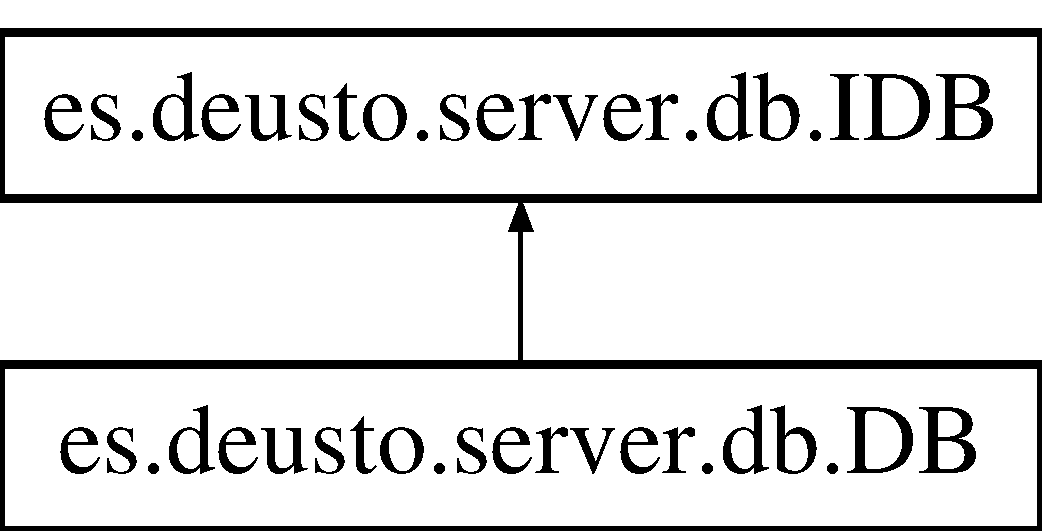
\includegraphics[height=2.000000cm]{classes_1_1deusto_1_1server_1_1db_1_1_d_b}
\end{center}
\end{figure}
\subsection*{Public Member Functions}
\begin{DoxyCompactItemize}
\item 
\hyperlink{classes_1_1deusto_1_1server_1_1db_1_1_d_b_ab53f32f36928ba9aa3ddff65fce395dc}{DB} ()
\item 
\hyperlink{classes_1_1deusto_1_1server_1_1db_1_1_d_b_a95f85fb4da6cf8b630f12536c81caaff}{DB} (\hyperlink{interfacees_1_1deusto_1_1server_1_1db_1_1dao_1_1_i_d_a_o}{I\+D\+AO} dao)
\item 
boolean \hyperlink{classes_1_1deusto_1_1server_1_1db_1_1_d_b_a8e5744311b5924e740d190673abee104}{login\+User} (\hyperlink{classes_1_1deusto_1_1server_1_1db_1_1data_1_1_user}{User} u)
\item 
boolean \hyperlink{classes_1_1deusto_1_1server_1_1db_1_1_d_b_a888f468b3fc2a05520fca9ac135823e3}{register\+User} (\hyperlink{classes_1_1deusto_1_1server_1_1db_1_1data_1_1_user}{User} u)
\item 
boolean \hyperlink{classes_1_1deusto_1_1server_1_1db_1_1_d_b_a8aa2e7531181a31b54850ca6665f87c2}{buy\+Game} (String username, String name)
\item 
List$<$ \hyperlink{classes_1_1deusto_1_1server_1_1db_1_1data_1_1_game}{Game} $>$ \hyperlink{classes_1_1deusto_1_1server_1_1db_1_1_d_b_ad878c1c58062596b5e1b582ed496bd11}{get\+All\+Games} ()
\item 
List$<$ \hyperlink{classes_1_1deusto_1_1server_1_1db_1_1data_1_1_game}{Game} $>$ \hyperlink{classes_1_1deusto_1_1server_1_1db_1_1_d_b_a1c471589284782e7ff1190f2b6c2369e}{get\+User\+Games} (String username)
\item 
List$<$ String $>$ \hyperlink{classes_1_1deusto_1_1server_1_1db_1_1_d_b_a59802aeefdd9d445152fbd548a964708}{get\+All\+Companies} ()
\item 
List$<$ String $>$ \hyperlink{classes_1_1deusto_1_1server_1_1db_1_1_d_b_a741c4c8b38c31010d5c86e1586ffa880}{get\+All\+Genres} ()
\item 
boolean \hyperlink{classes_1_1deusto_1_1server_1_1db_1_1_d_b_a376112d91f8e3018821fd9362f6598ae}{add\+Game\+To\+Db} (\hyperlink{classes_1_1deusto_1_1server_1_1db_1_1data_1_1_game}{Game} g, \hyperlink{classes_1_1deusto_1_1server_1_1db_1_1data_1_1_genre}{Genre} gg, \hyperlink{classes_1_1deusto_1_1server_1_1db_1_1data_1_1_company}{Company} c)
\item 
boolean \hyperlink{classes_1_1deusto_1_1server_1_1db_1_1_d_b_a53a59425c7690f07861fd5d006f83cbc}{is\+Super\+User} (String login)
\item 
\hyperlink{classes_1_1deusto_1_1server_1_1db_1_1data_1_1_user}{User} \hyperlink{classes_1_1deusto_1_1server_1_1db_1_1_d_b_ac85523faea523033439a932bbcab2c7e}{show\+User} (String login)
\item 
\hyperlink{classes_1_1deusto_1_1server_1_1db_1_1data_1_1_game}{Game} \hyperlink{classes_1_1deusto_1_1server_1_1db_1_1_d_b_adba76c20f2fc7ed01d486564d881a718}{show\+Game} (String name)
\item 
\hyperlink{classes_1_1deusto_1_1server_1_1db_1_1data_1_1_company}{Company} \hyperlink{classes_1_1deusto_1_1server_1_1db_1_1_d_b_ab5edf3ae158bb0501a882b1d724cc2a8}{show\+Company} (String name)
\item 
\hyperlink{classes_1_1deusto_1_1server_1_1db_1_1data_1_1_genre}{Genre} \hyperlink{classes_1_1deusto_1_1server_1_1db_1_1_d_b_a207ddeb183db925dc20f095033aa4d94}{show\+Genre} (String name)
\end{DoxyCompactItemize}


\subsection{Detailed Description}
This class executes all the basic functions of the database, such as buying a game, registering a user or adding a game for example \begin{DoxyAuthor}{Author}

\end{DoxyAuthor}
\begin{DoxyVersion}{Version}
1.\+0 
\end{DoxyVersion}
\begin{DoxySince}{Since}
24/03/2017 
\end{DoxySince}


Definition at line 24 of file D\+B.\+java.



\subsection{Constructor \& Destructor Documentation}
\mbox{\Hypertarget{classes_1_1deusto_1_1server_1_1db_1_1_d_b_ab53f32f36928ba9aa3ddff65fce395dc}\label{classes_1_1deusto_1_1server_1_1db_1_1_d_b_ab53f32f36928ba9aa3ddff65fce395dc}} 
\index{es\+::deusto\+::server\+::db\+::\+DB@{es\+::deusto\+::server\+::db\+::\+DB}!DB@{DB}}
\index{DB@{DB}!es\+::deusto\+::server\+::db\+::\+DB@{es\+::deusto\+::server\+::db\+::\+DB}}
\subsubsection{\texorpdfstring{D\+B()}{DB()}\hspace{0.1cm}{\footnotesize\ttfamily [1/2]}}
{\footnotesize\ttfamily es.\+deusto.\+server.\+db.\+D\+B.\+DB (\begin{DoxyParamCaption}{ }\end{DoxyParamCaption})}

This is the first constructor for the database 
\begin{DoxyParams}{Parameters}
{\em unused} & \\
\hline
\end{DoxyParams}
\begin{DoxyReturn}{Returns}
nothing 
\end{DoxyReturn}


Definition at line 37 of file D\+B.\+java.

\mbox{\Hypertarget{classes_1_1deusto_1_1server_1_1db_1_1_d_b_a95f85fb4da6cf8b630f12536c81caaff}\label{classes_1_1deusto_1_1server_1_1db_1_1_d_b_a95f85fb4da6cf8b630f12536c81caaff}} 
\index{es\+::deusto\+::server\+::db\+::\+DB@{es\+::deusto\+::server\+::db\+::\+DB}!DB@{DB}}
\index{DB@{DB}!es\+::deusto\+::server\+::db\+::\+DB@{es\+::deusto\+::server\+::db\+::\+DB}}
\subsubsection{\texorpdfstring{D\+B()}{DB()}\hspace{0.1cm}{\footnotesize\ttfamily [2/2]}}
{\footnotesize\ttfamily es.\+deusto.\+server.\+db.\+D\+B.\+DB (\begin{DoxyParamCaption}\item[{\hyperlink{interfacees_1_1deusto_1_1server_1_1db_1_1dao_1_1_i_d_a_o}{I\+D\+AO}}]{dao }\end{DoxyParamCaption})}

This is the second constructor for the database 
\begin{DoxyParams}{Parameters}
{\em udao} & This is the parameter to the constructor \\
\hline
\end{DoxyParams}
\begin{DoxyReturn}{Returns}
nothing 
\end{DoxyReturn}


Definition at line 46 of file D\+B.\+java.



\subsection{Member Function Documentation}
\mbox{\Hypertarget{classes_1_1deusto_1_1server_1_1db_1_1_d_b_a376112d91f8e3018821fd9362f6598ae}\label{classes_1_1deusto_1_1server_1_1db_1_1_d_b_a376112d91f8e3018821fd9362f6598ae}} 
\index{es\+::deusto\+::server\+::db\+::\+DB@{es\+::deusto\+::server\+::db\+::\+DB}!add\+Game\+To\+Db@{add\+Game\+To\+Db}}
\index{add\+Game\+To\+Db@{add\+Game\+To\+Db}!es\+::deusto\+::server\+::db\+::\+DB@{es\+::deusto\+::server\+::db\+::\+DB}}
\subsubsection{\texorpdfstring{add\+Game\+To\+Db()}{addGameToDb()}}
{\footnotesize\ttfamily boolean es.\+deusto.\+server.\+db.\+D\+B.\+add\+Game\+To\+Db (\begin{DoxyParamCaption}\item[{\hyperlink{classes_1_1deusto_1_1server_1_1db_1_1data_1_1_game}{Game}}]{g,  }\item[{\hyperlink{classes_1_1deusto_1_1server_1_1db_1_1data_1_1_genre}{Genre}}]{gg,  }\item[{\hyperlink{classes_1_1deusto_1_1server_1_1db_1_1data_1_1_company}{Company}}]{c }\end{DoxyParamCaption})}

This method adds a new game or updates a existing one into the database 
\begin{DoxyParams}{Parameters}
{\em g} & This is a game \\
\hline
{\em gg} & This is a genre \\
\hline
{\em c} & This is a company \\
\hline
\end{DoxyParams}
\begin{DoxyReturn}{Returns}
boolean Returns true or false depending on whether the game exists in the database or not 
\end{DoxyReturn}
\begin{DoxySeeAlso}{See also}
\hyperlink{interfacees_1_1deusto_1_1server_1_1db_1_1_i_d_b_a645335b2cbfa27c0199783ff2f33559e}{es.\+deusto.\+server.\+db.\+I\+D\+B\+::add\+Game\+To\+Db}(\hyperlink{classes_1_1deusto_1_1server_1_1db_1_1data_1_1_game}{es.\+deusto.\+server.\+db.\+data.\+Game}, \hyperlink{classes_1_1deusto_1_1server_1_1db_1_1data_1_1_genre}{es.\+deusto.\+server.\+db.\+data.\+Genre}, \hyperlink{classes_1_1deusto_1_1server_1_1db_1_1data_1_1_company}{es.\+deusto.\+server.\+db.\+data.\+Company}) 
\end{DoxySeeAlso}


Implements \hyperlink{interfacees_1_1deusto_1_1server_1_1db_1_1_i_d_b_a645335b2cbfa27c0199783ff2f33559e}{es.\+deusto.\+server.\+db.\+I\+DB}.



Definition at line 177 of file D\+B.\+java.

\mbox{\Hypertarget{classes_1_1deusto_1_1server_1_1db_1_1_d_b_a8aa2e7531181a31b54850ca6665f87c2}\label{classes_1_1deusto_1_1server_1_1db_1_1_d_b_a8aa2e7531181a31b54850ca6665f87c2}} 
\index{es\+::deusto\+::server\+::db\+::\+DB@{es\+::deusto\+::server\+::db\+::\+DB}!buy\+Game@{buy\+Game}}
\index{buy\+Game@{buy\+Game}!es\+::deusto\+::server\+::db\+::\+DB@{es\+::deusto\+::server\+::db\+::\+DB}}
\subsubsection{\texorpdfstring{buy\+Game()}{buyGame()}}
{\footnotesize\ttfamily boolean es.\+deusto.\+server.\+db.\+D\+B.\+buy\+Game (\begin{DoxyParamCaption}\item[{String}]{username,  }\item[{String}]{name }\end{DoxyParamCaption})}

Method that gives the user a license when buying a game 
\begin{DoxyParams}{Parameters}
{\em username} & This is the login username of a user \\
\hline
{\em name} & This is the name of a game \\
\hline
\end{DoxyParams}
\begin{DoxyReturn}{Returns}
boolean Returns true when the user has the license 
\end{DoxyReturn}
\begin{DoxySeeAlso}{See also}
\hyperlink{interfacees_1_1deusto_1_1server_1_1db_1_1_i_d_b_ab1076d02bd6b4da29d0e99e1310048b6}{es.\+deusto.\+server.\+db.\+I\+D\+B\+::buy\+Game}(java.\+lang.\+String, java.\+lang.\+String) 
\end{DoxySeeAlso}


Implements \hyperlink{interfacees_1_1deusto_1_1server_1_1db_1_1_i_d_b_ab1076d02bd6b4da29d0e99e1310048b6}{es.\+deusto.\+server.\+db.\+I\+DB}.



Definition at line 96 of file D\+B.\+java.

\mbox{\Hypertarget{classes_1_1deusto_1_1server_1_1db_1_1_d_b_a59802aeefdd9d445152fbd548a964708}\label{classes_1_1deusto_1_1server_1_1db_1_1_d_b_a59802aeefdd9d445152fbd548a964708}} 
\index{es\+::deusto\+::server\+::db\+::\+DB@{es\+::deusto\+::server\+::db\+::\+DB}!get\+All\+Companies@{get\+All\+Companies}}
\index{get\+All\+Companies@{get\+All\+Companies}!es\+::deusto\+::server\+::db\+::\+DB@{es\+::deusto\+::server\+::db\+::\+DB}}
\subsubsection{\texorpdfstring{get\+All\+Companies()}{getAllCompanies()}}
{\footnotesize\ttfamily List$<$String$>$ es.\+deusto.\+server.\+db.\+D\+B.\+get\+All\+Companies (\begin{DoxyParamCaption}{ }\end{DoxyParamCaption})}

This method shows a list of companies 
\begin{DoxyParams}{Parameters}
{\em unused} & \\
\hline
\end{DoxyParams}
\begin{DoxyReturn}{Returns}
List Returns a list of companies 
\end{DoxyReturn}
\begin{DoxySeeAlso}{See also}
\hyperlink{interfacees_1_1deusto_1_1server_1_1db_1_1_i_d_b_af7500b1f7c74d658837ed1a5ec82ebec}{es.\+deusto.\+server.\+db.\+I\+D\+B\+::get\+All\+Companies()} 
\end{DoxySeeAlso}


Implements \hyperlink{interfacees_1_1deusto_1_1server_1_1db_1_1_i_d_b_af7500b1f7c74d658837ed1a5ec82ebec}{es.\+deusto.\+server.\+db.\+I\+DB}.



Definition at line 145 of file D\+B.\+java.

\mbox{\Hypertarget{classes_1_1deusto_1_1server_1_1db_1_1_d_b_ad878c1c58062596b5e1b582ed496bd11}\label{classes_1_1deusto_1_1server_1_1db_1_1_d_b_ad878c1c58062596b5e1b582ed496bd11}} 
\index{es\+::deusto\+::server\+::db\+::\+DB@{es\+::deusto\+::server\+::db\+::\+DB}!get\+All\+Games@{get\+All\+Games}}
\index{get\+All\+Games@{get\+All\+Games}!es\+::deusto\+::server\+::db\+::\+DB@{es\+::deusto\+::server\+::db\+::\+DB}}
\subsubsection{\texorpdfstring{get\+All\+Games()}{getAllGames()}}
{\footnotesize\ttfamily List$<$\hyperlink{classes_1_1deusto_1_1server_1_1db_1_1data_1_1_game}{Game}$>$ es.\+deusto.\+server.\+db.\+D\+B.\+get\+All\+Games (\begin{DoxyParamCaption}{ }\end{DoxyParamCaption})}

This method shows a list of games 
\begin{DoxyParams}{Parameters}
{\em unused} & \\
\hline
\end{DoxyParams}
\begin{DoxyReturn}{Returns}
List Returns a list of games 
\end{DoxyReturn}
\begin{DoxySeeAlso}{See also}
\hyperlink{interfacees_1_1deusto_1_1server_1_1db_1_1_i_d_b_a76af81d4bb71c81490da92d67c5b6d03}{es.\+deusto.\+server.\+db.\+I\+D\+B\+::get\+All\+Games()} 
\end{DoxySeeAlso}


Implements \hyperlink{interfacees_1_1deusto_1_1server_1_1db_1_1_i_d_b_a76af81d4bb71c81490da92d67c5b6d03}{es.\+deusto.\+server.\+db.\+I\+DB}.



Definition at line 120 of file D\+B.\+java.

\mbox{\Hypertarget{classes_1_1deusto_1_1server_1_1db_1_1_d_b_a741c4c8b38c31010d5c86e1586ffa880}\label{classes_1_1deusto_1_1server_1_1db_1_1_d_b_a741c4c8b38c31010d5c86e1586ffa880}} 
\index{es\+::deusto\+::server\+::db\+::\+DB@{es\+::deusto\+::server\+::db\+::\+DB}!get\+All\+Genres@{get\+All\+Genres}}
\index{get\+All\+Genres@{get\+All\+Genres}!es\+::deusto\+::server\+::db\+::\+DB@{es\+::deusto\+::server\+::db\+::\+DB}}
\subsubsection{\texorpdfstring{get\+All\+Genres()}{getAllGenres()}}
{\footnotesize\ttfamily List$<$String$>$ es.\+deusto.\+server.\+db.\+D\+B.\+get\+All\+Genres (\begin{DoxyParamCaption}{ }\end{DoxyParamCaption})}

This method shows a list of genres 
\begin{DoxyParams}{Parameters}
{\em unused} & \\
\hline
\end{DoxyParams}
\begin{DoxyReturn}{Returns}
List Returns a list of genres 
\end{DoxyReturn}
\begin{DoxySeeAlso}{See also}
\hyperlink{interfacees_1_1deusto_1_1server_1_1db_1_1_i_d_b_ab0d82284b373b0ea3e0c441892e678b5}{es.\+deusto.\+server.\+db.\+I\+D\+B\+::get\+All\+Genres()} 
\end{DoxySeeAlso}


Implements \hyperlink{interfacees_1_1deusto_1_1server_1_1db_1_1_i_d_b_ab0d82284b373b0ea3e0c441892e678b5}{es.\+deusto.\+server.\+db.\+I\+DB}.



Definition at line 160 of file D\+B.\+java.

\mbox{\Hypertarget{classes_1_1deusto_1_1server_1_1db_1_1_d_b_a1c471589284782e7ff1190f2b6c2369e}\label{classes_1_1deusto_1_1server_1_1db_1_1_d_b_a1c471589284782e7ff1190f2b6c2369e}} 
\index{es\+::deusto\+::server\+::db\+::\+DB@{es\+::deusto\+::server\+::db\+::\+DB}!get\+User\+Games@{get\+User\+Games}}
\index{get\+User\+Games@{get\+User\+Games}!es\+::deusto\+::server\+::db\+::\+DB@{es\+::deusto\+::server\+::db\+::\+DB}}
\subsubsection{\texorpdfstring{get\+User\+Games()}{getUserGames()}}
{\footnotesize\ttfamily List$<$\hyperlink{classes_1_1deusto_1_1server_1_1db_1_1data_1_1_game}{Game}$>$ es.\+deusto.\+server.\+db.\+D\+B.\+get\+User\+Games (\begin{DoxyParamCaption}\item[{String}]{username }\end{DoxyParamCaption})}

Method that returns the list of games of a user 
\begin{DoxyParams}{Parameters}
{\em username} & This is the login username of a user \\
\hline
\end{DoxyParams}
\begin{DoxyReturn}{Returns}
list Returns a list of games 
\end{DoxyReturn}
\begin{DoxySeeAlso}{See also}
\hyperlink{interfacees_1_1deusto_1_1server_1_1db_1_1_i_d_b_ac5ef9780a640140576f9373f8b57631c}{es.\+deusto.\+server.\+db.\+I\+D\+B\+::get\+User\+Games}(java.\+lang.\+String) 
\end{DoxySeeAlso}


Implements \hyperlink{interfacees_1_1deusto_1_1server_1_1db_1_1_i_d_b_ac5ef9780a640140576f9373f8b57631c}{es.\+deusto.\+server.\+db.\+I\+DB}.



Definition at line 130 of file D\+B.\+java.

\mbox{\Hypertarget{classes_1_1deusto_1_1server_1_1db_1_1_d_b_a53a59425c7690f07861fd5d006f83cbc}\label{classes_1_1deusto_1_1server_1_1db_1_1_d_b_a53a59425c7690f07861fd5d006f83cbc}} 
\index{es\+::deusto\+::server\+::db\+::\+DB@{es\+::deusto\+::server\+::db\+::\+DB}!is\+Super\+User@{is\+Super\+User}}
\index{is\+Super\+User@{is\+Super\+User}!es\+::deusto\+::server\+::db\+::\+DB@{es\+::deusto\+::server\+::db\+::\+DB}}
\subsubsection{\texorpdfstring{is\+Super\+User()}{isSuperUser()}}
{\footnotesize\ttfamily boolean es.\+deusto.\+server.\+db.\+D\+B.\+is\+Super\+User (\begin{DoxyParamCaption}\item[{String}]{login }\end{DoxyParamCaption})}

This method shows if a user is also superuser or not 
\begin{DoxyParams}{Parameters}
{\em login} & This is the login name of a user \\
\hline
\end{DoxyParams}
\begin{DoxyReturn}{Returns}
boolean Returns if a user is superuser or not 
\end{DoxyReturn}
\begin{DoxySeeAlso}{See also}
\hyperlink{interfacees_1_1deusto_1_1server_1_1db_1_1_i_d_b_a279d8a59498d4157f2d20ce7f0c4cfdb}{es.\+deusto.\+server.\+db.\+I\+D\+B\+::is\+Super\+User}(java.\+lang.\+String) 
\end{DoxySeeAlso}


Implements \hyperlink{interfacees_1_1deusto_1_1server_1_1db_1_1_i_d_b_a279d8a59498d4157f2d20ce7f0c4cfdb}{es.\+deusto.\+server.\+db.\+I\+DB}.



Definition at line 240 of file D\+B.\+java.

\mbox{\Hypertarget{classes_1_1deusto_1_1server_1_1db_1_1_d_b_a8e5744311b5924e740d190673abee104}\label{classes_1_1deusto_1_1server_1_1db_1_1_d_b_a8e5744311b5924e740d190673abee104}} 
\index{es\+::deusto\+::server\+::db\+::\+DB@{es\+::deusto\+::server\+::db\+::\+DB}!login\+User@{login\+User}}
\index{login\+User@{login\+User}!es\+::deusto\+::server\+::db\+::\+DB@{es\+::deusto\+::server\+::db\+::\+DB}}
\subsubsection{\texorpdfstring{login\+User()}{loginUser()}}
{\footnotesize\ttfamily boolean es.\+deusto.\+server.\+db.\+D\+B.\+login\+User (\begin{DoxyParamCaption}\item[{\hyperlink{classes_1_1deusto_1_1server_1_1db_1_1data_1_1_user}{User}}]{u }\end{DoxyParamCaption})}

This method allows the user to log in 
\begin{DoxyParams}{Parameters}
{\em u} & This is a user \\
\hline
\end{DoxyParams}
\begin{DoxyReturn}{Returns}
boolean Returns true or false depending on whether the user exists or not 
\end{DoxyReturn}
\begin{DoxySeeAlso}{See also}
\hyperlink{interfacees_1_1deusto_1_1server_1_1db_1_1_i_d_b_a6e6196e5899fc93134223373ed8363a6}{es.\+deusto.\+server.\+db.\+I\+D\+B\+::login\+User}(\hyperlink{classes_1_1deusto_1_1server_1_1db_1_1data_1_1_user}{es.\+deusto.\+server.\+db.\+data.\+User}) 
\end{DoxySeeAlso}


Implements \hyperlink{interfacees_1_1deusto_1_1server_1_1db_1_1_i_d_b_a6e6196e5899fc93134223373ed8363a6}{es.\+deusto.\+server.\+db.\+I\+DB}.



Definition at line 58 of file D\+B.\+java.

\mbox{\Hypertarget{classes_1_1deusto_1_1server_1_1db_1_1_d_b_a888f468b3fc2a05520fca9ac135823e3}\label{classes_1_1deusto_1_1server_1_1db_1_1_d_b_a888f468b3fc2a05520fca9ac135823e3}} 
\index{es\+::deusto\+::server\+::db\+::\+DB@{es\+::deusto\+::server\+::db\+::\+DB}!register\+User@{register\+User}}
\index{register\+User@{register\+User}!es\+::deusto\+::server\+::db\+::\+DB@{es\+::deusto\+::server\+::db\+::\+DB}}
\subsubsection{\texorpdfstring{register\+User()}{registerUser()}}
{\footnotesize\ttfamily boolean es.\+deusto.\+server.\+db.\+D\+B.\+register\+User (\begin{DoxyParamCaption}\item[{\hyperlink{classes_1_1deusto_1_1server_1_1db_1_1data_1_1_user}{User}}]{u }\end{DoxyParamCaption})}

This method saves a new user 
\begin{DoxyParams}{Parameters}
{\em u} & This is a user \\
\hline
\end{DoxyParams}
\begin{DoxyReturn}{Returns}
boolean Returns true or false depending on whether the user exists or not 
\end{DoxyReturn}
\begin{DoxySeeAlso}{See also}
\hyperlink{interfacees_1_1deusto_1_1server_1_1db_1_1_i_d_b_ad9ecf628cb97ade7cb1b10fd1b3a18c4}{es.\+deusto.\+server.\+db.\+I\+D\+B\+::register\+User}(\hyperlink{classes_1_1deusto_1_1server_1_1db_1_1data_1_1_user}{es.\+deusto.\+server.\+db.\+data.\+User}) 
\end{DoxySeeAlso}


Implements \hyperlink{interfacees_1_1deusto_1_1server_1_1db_1_1_i_d_b_ad9ecf628cb97ade7cb1b10fd1b3a18c4}{es.\+deusto.\+server.\+db.\+I\+DB}.



Definition at line 79 of file D\+B.\+java.

\mbox{\Hypertarget{classes_1_1deusto_1_1server_1_1db_1_1_d_b_ab5edf3ae158bb0501a882b1d724cc2a8}\label{classes_1_1deusto_1_1server_1_1db_1_1_d_b_ab5edf3ae158bb0501a882b1d724cc2a8}} 
\index{es\+::deusto\+::server\+::db\+::\+DB@{es\+::deusto\+::server\+::db\+::\+DB}!show\+Company@{show\+Company}}
\index{show\+Company@{show\+Company}!es\+::deusto\+::server\+::db\+::\+DB@{es\+::deusto\+::server\+::db\+::\+DB}}
\subsubsection{\texorpdfstring{show\+Company()}{showCompany()}}
{\footnotesize\ttfamily \hyperlink{classes_1_1deusto_1_1server_1_1db_1_1data_1_1_company}{Company} es.\+deusto.\+server.\+db.\+D\+B.\+show\+Company (\begin{DoxyParamCaption}\item[{String}]{name }\end{DoxyParamCaption})}

This method shows the company of a game 
\begin{DoxyParams}{Parameters}
{\em name} & This is the name of a company \\
\hline
\end{DoxyParams}
\begin{DoxyReturn}{Returns}
Company Returns the company of a game 
\end{DoxyReturn}
\begin{DoxySeeAlso}{See also}
\hyperlink{interfacees_1_1deusto_1_1server_1_1db_1_1_i_d_b_a1681e29b5fbe4377b19e67fa939b2782}{es.\+deusto.\+server.\+db.\+I\+D\+B\+::show\+Company}(java.\+lang.\+String) 
\end{DoxySeeAlso}


Implements \hyperlink{interfacees_1_1deusto_1_1server_1_1db_1_1_i_d_b_a1681e29b5fbe4377b19e67fa939b2782}{es.\+deusto.\+server.\+db.\+I\+DB}.



Definition at line 271 of file D\+B.\+java.

\mbox{\Hypertarget{classes_1_1deusto_1_1server_1_1db_1_1_d_b_adba76c20f2fc7ed01d486564d881a718}\label{classes_1_1deusto_1_1server_1_1db_1_1_d_b_adba76c20f2fc7ed01d486564d881a718}} 
\index{es\+::deusto\+::server\+::db\+::\+DB@{es\+::deusto\+::server\+::db\+::\+DB}!show\+Game@{show\+Game}}
\index{show\+Game@{show\+Game}!es\+::deusto\+::server\+::db\+::\+DB@{es\+::deusto\+::server\+::db\+::\+DB}}
\subsubsection{\texorpdfstring{show\+Game()}{showGame()}}
{\footnotesize\ttfamily \hyperlink{classes_1_1deusto_1_1server_1_1db_1_1data_1_1_game}{Game} es.\+deusto.\+server.\+db.\+D\+B.\+show\+Game (\begin{DoxyParamCaption}\item[{String}]{name }\end{DoxyParamCaption})}

This method shows a game 
\begin{DoxyParams}{Parameters}
{\em name} & This is the name of a game return Game Returns a game \\
\hline
\end{DoxyParams}
\begin{DoxySeeAlso}{See also}
\hyperlink{interfacees_1_1deusto_1_1server_1_1db_1_1_i_d_b_a572028cc62d36bebee977200b55eba8b}{es.\+deusto.\+server.\+db.\+I\+D\+B\+::show\+Game}(java.\+lang.\+String) 
\end{DoxySeeAlso}


Implements \hyperlink{interfacees_1_1deusto_1_1server_1_1db_1_1_i_d_b_a572028cc62d36bebee977200b55eba8b}{es.\+deusto.\+server.\+db.\+I\+DB}.



Definition at line 259 of file D\+B.\+java.

\mbox{\Hypertarget{classes_1_1deusto_1_1server_1_1db_1_1_d_b_a207ddeb183db925dc20f095033aa4d94}\label{classes_1_1deusto_1_1server_1_1db_1_1_d_b_a207ddeb183db925dc20f095033aa4d94}} 
\index{es\+::deusto\+::server\+::db\+::\+DB@{es\+::deusto\+::server\+::db\+::\+DB}!show\+Genre@{show\+Genre}}
\index{show\+Genre@{show\+Genre}!es\+::deusto\+::server\+::db\+::\+DB@{es\+::deusto\+::server\+::db\+::\+DB}}
\subsubsection{\texorpdfstring{show\+Genre()}{showGenre()}}
{\footnotesize\ttfamily \hyperlink{classes_1_1deusto_1_1server_1_1db_1_1data_1_1_genre}{Genre} es.\+deusto.\+server.\+db.\+D\+B.\+show\+Genre (\begin{DoxyParamCaption}\item[{String}]{name }\end{DoxyParamCaption})}

This method shows the genre of a game 
\begin{DoxyParams}{Parameters}
{\em name} & This is the name of a genre \\
\hline
\end{DoxyParams}
\begin{DoxyReturn}{Returns}
Genre Returns the genre of a game 
\end{DoxyReturn}
\begin{DoxySeeAlso}{See also}
\hyperlink{interfacees_1_1deusto_1_1server_1_1db_1_1_i_d_b_a9023bdad77781d95fc2e556d1935f763}{es.\+deusto.\+server.\+db.\+I\+D\+B\+::show\+Genre}(java.\+lang.\+String) 
\end{DoxySeeAlso}


Implements \hyperlink{interfacees_1_1deusto_1_1server_1_1db_1_1_i_d_b_a9023bdad77781d95fc2e556d1935f763}{es.\+deusto.\+server.\+db.\+I\+DB}.



Definition at line 283 of file D\+B.\+java.

\mbox{\Hypertarget{classes_1_1deusto_1_1server_1_1db_1_1_d_b_ac85523faea523033439a932bbcab2c7e}\label{classes_1_1deusto_1_1server_1_1db_1_1_d_b_ac85523faea523033439a932bbcab2c7e}} 
\index{es\+::deusto\+::server\+::db\+::\+DB@{es\+::deusto\+::server\+::db\+::\+DB}!show\+User@{show\+User}}
\index{show\+User@{show\+User}!es\+::deusto\+::server\+::db\+::\+DB@{es\+::deusto\+::server\+::db\+::\+DB}}
\subsubsection{\texorpdfstring{show\+User()}{showUser()}}
{\footnotesize\ttfamily \hyperlink{classes_1_1deusto_1_1server_1_1db_1_1data_1_1_user}{User} es.\+deusto.\+server.\+db.\+D\+B.\+show\+User (\begin{DoxyParamCaption}\item[{String}]{login }\end{DoxyParamCaption})}



Implements \hyperlink{interfacees_1_1deusto_1_1server_1_1db_1_1_i_d_b_aa2f6a5291fa8aa78d5a73b5878d17986}{es.\+deusto.\+server.\+db.\+I\+DB}.



Definition at line 247 of file D\+B.\+java.



The documentation for this class was generated from the following file\+:\begin{DoxyCompactItemize}
\item 
src/main/java/es/deusto/server/db/\hyperlink{_d_b_8java}{D\+B.\+java}\end{DoxyCompactItemize}

\hypertarget{classes_1_1deusto_1_1server_1_1db_1_1data_1_1_game}{}\section{es.\+deusto.\+server.\+db.\+data.\+Game Class Reference}
\label{classes_1_1deusto_1_1server_1_1db_1_1data_1_1_game}\index{es.\+deusto.\+server.\+db.\+data.\+Game@{es.\+deusto.\+server.\+db.\+data.\+Game}}
Inheritance diagram for es.\+deusto.\+server.\+db.\+data.\+Game\+:\begin{figure}[H]
\begin{center}
\leavevmode
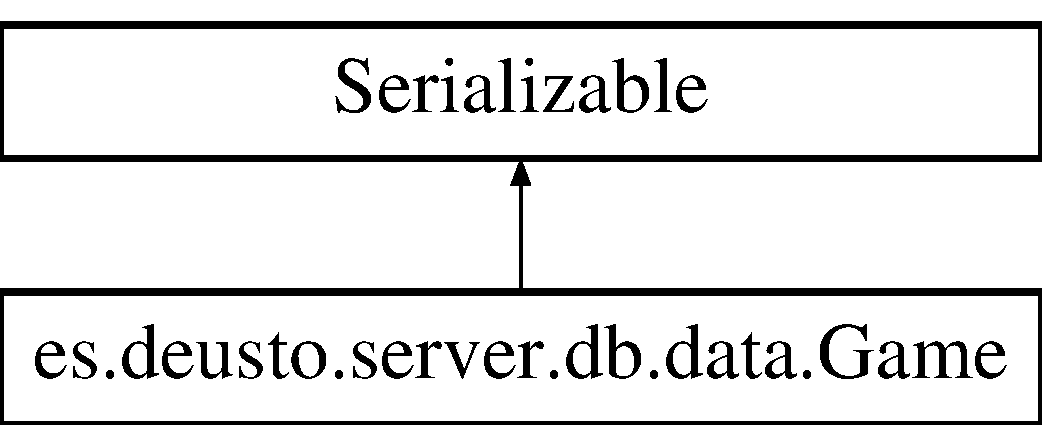
\includegraphics[height=2.000000cm]{classes_1_1deusto_1_1server_1_1db_1_1data_1_1_game}
\end{center}
\end{figure}
\subsection*{Public Member Functions}
\begin{DoxyCompactItemize}
\item 
\hyperlink{classes_1_1deusto_1_1server_1_1db_1_1data_1_1_game_aad926d06e556453f4b08efa5a3e620d4}{Game} (String name, double price, double discount)
\item 
String \hyperlink{classes_1_1deusto_1_1server_1_1db_1_1data_1_1_game_af9f6defe43d11cefdef169a6aaa87ae7}{get\+Name} ()
\item 
double \hyperlink{classes_1_1deusto_1_1server_1_1db_1_1data_1_1_game_a1b39bf61a9699d6bdd013e48d1159def}{get\+Price} ()
\item 
double \hyperlink{classes_1_1deusto_1_1server_1_1db_1_1data_1_1_game_a4c75cd53d5bd16c62804ca3779440165}{get\+Discount} ()
\item 
void \hyperlink{classes_1_1deusto_1_1server_1_1db_1_1data_1_1_game_aaa7e3ebbc4cd3b62080b39c98d374424}{add\+License} (\hyperlink{classes_1_1deusto_1_1server_1_1db_1_1data_1_1_license}{License} license)
\item 
void \hyperlink{classes_1_1deusto_1_1server_1_1db_1_1data_1_1_game_a4ca6c0283ef51e95fbed8f52fd76d985}{remove\+License} (\hyperlink{classes_1_1deusto_1_1server_1_1db_1_1data_1_1_license}{License} license)
\item 
List$<$ \hyperlink{classes_1_1deusto_1_1server_1_1db_1_1data_1_1_license}{License} $>$ \hyperlink{classes_1_1deusto_1_1server_1_1db_1_1data_1_1_game_a6da5b38821b5c9bcb71b26721af09bf0}{get\+Licenses} ()
\item 
\hyperlink{classes_1_1deusto_1_1server_1_1db_1_1data_1_1_genre}{Genre} \hyperlink{classes_1_1deusto_1_1server_1_1db_1_1data_1_1_game_a021c30dd22681130bbdb6f2690ba8657}{get\+Genre} ()
\item 
void \hyperlink{classes_1_1deusto_1_1server_1_1db_1_1data_1_1_game_a61d197148280723f018c7ef18e37cb7e}{set\+Genre} (\hyperlink{classes_1_1deusto_1_1server_1_1db_1_1data_1_1_genre}{Genre} genre)
\item 
\hyperlink{classes_1_1deusto_1_1server_1_1db_1_1data_1_1_company}{Company} \hyperlink{classes_1_1deusto_1_1server_1_1db_1_1data_1_1_game_aa772f16e7094839759148d49a4634e82}{get\+Company} ()
\item 
void \hyperlink{classes_1_1deusto_1_1server_1_1db_1_1data_1_1_game_a3699723b19412f250feea6e9c730815c}{set\+Company} (\hyperlink{classes_1_1deusto_1_1server_1_1db_1_1data_1_1_company}{Company} company)
\item 
String \hyperlink{classes_1_1deusto_1_1server_1_1db_1_1data_1_1_game_aae9eb6e19b8f730b9554cfac23c8298b}{to\+String} ()
\end{DoxyCompactItemize}


\subsection{Detailed Description}


Definition at line 19 of file Game.\+java.



\subsection{Constructor \& Destructor Documentation}
\mbox{\Hypertarget{classes_1_1deusto_1_1server_1_1db_1_1data_1_1_game_aad926d06e556453f4b08efa5a3e620d4}\label{classes_1_1deusto_1_1server_1_1db_1_1data_1_1_game_aad926d06e556453f4b08efa5a3e620d4}} 
\index{es\+::deusto\+::server\+::db\+::data\+::\+Game@{es\+::deusto\+::server\+::db\+::data\+::\+Game}!Game@{Game}}
\index{Game@{Game}!es\+::deusto\+::server\+::db\+::data\+::\+Game@{es\+::deusto\+::server\+::db\+::data\+::\+Game}}
\subsubsection{\texorpdfstring{Game()}{Game()}}
{\footnotesize\ttfamily es.\+deusto.\+server.\+db.\+data.\+Game.\+Game (\begin{DoxyParamCaption}\item[{String}]{name,  }\item[{double}]{price,  }\item[{double}]{discount }\end{DoxyParamCaption})}



Definition at line 35 of file Game.\+java.



\subsection{Member Function Documentation}
\mbox{\Hypertarget{classes_1_1deusto_1_1server_1_1db_1_1data_1_1_game_aaa7e3ebbc4cd3b62080b39c98d374424}\label{classes_1_1deusto_1_1server_1_1db_1_1data_1_1_game_aaa7e3ebbc4cd3b62080b39c98d374424}} 
\index{es\+::deusto\+::server\+::db\+::data\+::\+Game@{es\+::deusto\+::server\+::db\+::data\+::\+Game}!add\+License@{add\+License}}
\index{add\+License@{add\+License}!es\+::deusto\+::server\+::db\+::data\+::\+Game@{es\+::deusto\+::server\+::db\+::data\+::\+Game}}
\subsubsection{\texorpdfstring{add\+License()}{addLicense()}}
{\footnotesize\ttfamily void es.\+deusto.\+server.\+db.\+data.\+Game.\+add\+License (\begin{DoxyParamCaption}\item[{\hyperlink{classes_1_1deusto_1_1server_1_1db_1_1data_1_1_license}{License}}]{license }\end{DoxyParamCaption})}



Definition at line 53 of file Game.\+java.

\mbox{\Hypertarget{classes_1_1deusto_1_1server_1_1db_1_1data_1_1_game_aa772f16e7094839759148d49a4634e82}\label{classes_1_1deusto_1_1server_1_1db_1_1data_1_1_game_aa772f16e7094839759148d49a4634e82}} 
\index{es\+::deusto\+::server\+::db\+::data\+::\+Game@{es\+::deusto\+::server\+::db\+::data\+::\+Game}!get\+Company@{get\+Company}}
\index{get\+Company@{get\+Company}!es\+::deusto\+::server\+::db\+::data\+::\+Game@{es\+::deusto\+::server\+::db\+::data\+::\+Game}}
\subsubsection{\texorpdfstring{get\+Company()}{getCompany()}}
{\footnotesize\ttfamily \hyperlink{classes_1_1deusto_1_1server_1_1db_1_1data_1_1_company}{Company} es.\+deusto.\+server.\+db.\+data.\+Game.\+get\+Company (\begin{DoxyParamCaption}{ }\end{DoxyParamCaption})}



Definition at line 73 of file Game.\+java.

\mbox{\Hypertarget{classes_1_1deusto_1_1server_1_1db_1_1data_1_1_game_a4c75cd53d5bd16c62804ca3779440165}\label{classes_1_1deusto_1_1server_1_1db_1_1data_1_1_game_a4c75cd53d5bd16c62804ca3779440165}} 
\index{es\+::deusto\+::server\+::db\+::data\+::\+Game@{es\+::deusto\+::server\+::db\+::data\+::\+Game}!get\+Discount@{get\+Discount}}
\index{get\+Discount@{get\+Discount}!es\+::deusto\+::server\+::db\+::data\+::\+Game@{es\+::deusto\+::server\+::db\+::data\+::\+Game}}
\subsubsection{\texorpdfstring{get\+Discount()}{getDiscount()}}
{\footnotesize\ttfamily double es.\+deusto.\+server.\+db.\+data.\+Game.\+get\+Discount (\begin{DoxyParamCaption}{ }\end{DoxyParamCaption})}



Definition at line 49 of file Game.\+java.

\mbox{\Hypertarget{classes_1_1deusto_1_1server_1_1db_1_1data_1_1_game_a021c30dd22681130bbdb6f2690ba8657}\label{classes_1_1deusto_1_1server_1_1db_1_1data_1_1_game_a021c30dd22681130bbdb6f2690ba8657}} 
\index{es\+::deusto\+::server\+::db\+::data\+::\+Game@{es\+::deusto\+::server\+::db\+::data\+::\+Game}!get\+Genre@{get\+Genre}}
\index{get\+Genre@{get\+Genre}!es\+::deusto\+::server\+::db\+::data\+::\+Game@{es\+::deusto\+::server\+::db\+::data\+::\+Game}}
\subsubsection{\texorpdfstring{get\+Genre()}{getGenre()}}
{\footnotesize\ttfamily \hyperlink{classes_1_1deusto_1_1server_1_1db_1_1data_1_1_genre}{Genre} es.\+deusto.\+server.\+db.\+data.\+Game.\+get\+Genre (\begin{DoxyParamCaption}{ }\end{DoxyParamCaption})}



Definition at line 65 of file Game.\+java.

\mbox{\Hypertarget{classes_1_1deusto_1_1server_1_1db_1_1data_1_1_game_a6da5b38821b5c9bcb71b26721af09bf0}\label{classes_1_1deusto_1_1server_1_1db_1_1data_1_1_game_a6da5b38821b5c9bcb71b26721af09bf0}} 
\index{es\+::deusto\+::server\+::db\+::data\+::\+Game@{es\+::deusto\+::server\+::db\+::data\+::\+Game}!get\+Licenses@{get\+Licenses}}
\index{get\+Licenses@{get\+Licenses}!es\+::deusto\+::server\+::db\+::data\+::\+Game@{es\+::deusto\+::server\+::db\+::data\+::\+Game}}
\subsubsection{\texorpdfstring{get\+Licenses()}{getLicenses()}}
{\footnotesize\ttfamily List$<$\hyperlink{classes_1_1deusto_1_1server_1_1db_1_1data_1_1_license}{License}$>$ es.\+deusto.\+server.\+db.\+data.\+Game.\+get\+Licenses (\begin{DoxyParamCaption}{ }\end{DoxyParamCaption})}



Definition at line 61 of file Game.\+java.

\mbox{\Hypertarget{classes_1_1deusto_1_1server_1_1db_1_1data_1_1_game_af9f6defe43d11cefdef169a6aaa87ae7}\label{classes_1_1deusto_1_1server_1_1db_1_1data_1_1_game_af9f6defe43d11cefdef169a6aaa87ae7}} 
\index{es\+::deusto\+::server\+::db\+::data\+::\+Game@{es\+::deusto\+::server\+::db\+::data\+::\+Game}!get\+Name@{get\+Name}}
\index{get\+Name@{get\+Name}!es\+::deusto\+::server\+::db\+::data\+::\+Game@{es\+::deusto\+::server\+::db\+::data\+::\+Game}}
\subsubsection{\texorpdfstring{get\+Name()}{getName()}}
{\footnotesize\ttfamily String es.\+deusto.\+server.\+db.\+data.\+Game.\+get\+Name (\begin{DoxyParamCaption}{ }\end{DoxyParamCaption})}



Definition at line 41 of file Game.\+java.

\mbox{\Hypertarget{classes_1_1deusto_1_1server_1_1db_1_1data_1_1_game_a1b39bf61a9699d6bdd013e48d1159def}\label{classes_1_1deusto_1_1server_1_1db_1_1data_1_1_game_a1b39bf61a9699d6bdd013e48d1159def}} 
\index{es\+::deusto\+::server\+::db\+::data\+::\+Game@{es\+::deusto\+::server\+::db\+::data\+::\+Game}!get\+Price@{get\+Price}}
\index{get\+Price@{get\+Price}!es\+::deusto\+::server\+::db\+::data\+::\+Game@{es\+::deusto\+::server\+::db\+::data\+::\+Game}}
\subsubsection{\texorpdfstring{get\+Price()}{getPrice()}}
{\footnotesize\ttfamily double es.\+deusto.\+server.\+db.\+data.\+Game.\+get\+Price (\begin{DoxyParamCaption}{ }\end{DoxyParamCaption})}



Definition at line 45 of file Game.\+java.

\mbox{\Hypertarget{classes_1_1deusto_1_1server_1_1db_1_1data_1_1_game_a4ca6c0283ef51e95fbed8f52fd76d985}\label{classes_1_1deusto_1_1server_1_1db_1_1data_1_1_game_a4ca6c0283ef51e95fbed8f52fd76d985}} 
\index{es\+::deusto\+::server\+::db\+::data\+::\+Game@{es\+::deusto\+::server\+::db\+::data\+::\+Game}!remove\+License@{remove\+License}}
\index{remove\+License@{remove\+License}!es\+::deusto\+::server\+::db\+::data\+::\+Game@{es\+::deusto\+::server\+::db\+::data\+::\+Game}}
\subsubsection{\texorpdfstring{remove\+License()}{removeLicense()}}
{\footnotesize\ttfamily void es.\+deusto.\+server.\+db.\+data.\+Game.\+remove\+License (\begin{DoxyParamCaption}\item[{\hyperlink{classes_1_1deusto_1_1server_1_1db_1_1data_1_1_license}{License}}]{license }\end{DoxyParamCaption})}



Definition at line 57 of file Game.\+java.

\mbox{\Hypertarget{classes_1_1deusto_1_1server_1_1db_1_1data_1_1_game_a3699723b19412f250feea6e9c730815c}\label{classes_1_1deusto_1_1server_1_1db_1_1data_1_1_game_a3699723b19412f250feea6e9c730815c}} 
\index{es\+::deusto\+::server\+::db\+::data\+::\+Game@{es\+::deusto\+::server\+::db\+::data\+::\+Game}!set\+Company@{set\+Company}}
\index{set\+Company@{set\+Company}!es\+::deusto\+::server\+::db\+::data\+::\+Game@{es\+::deusto\+::server\+::db\+::data\+::\+Game}}
\subsubsection{\texorpdfstring{set\+Company()}{setCompany()}}
{\footnotesize\ttfamily void es.\+deusto.\+server.\+db.\+data.\+Game.\+set\+Company (\begin{DoxyParamCaption}\item[{\hyperlink{classes_1_1deusto_1_1server_1_1db_1_1data_1_1_company}{Company}}]{company }\end{DoxyParamCaption})}



Definition at line 77 of file Game.\+java.

\mbox{\Hypertarget{classes_1_1deusto_1_1server_1_1db_1_1data_1_1_game_a61d197148280723f018c7ef18e37cb7e}\label{classes_1_1deusto_1_1server_1_1db_1_1data_1_1_game_a61d197148280723f018c7ef18e37cb7e}} 
\index{es\+::deusto\+::server\+::db\+::data\+::\+Game@{es\+::deusto\+::server\+::db\+::data\+::\+Game}!set\+Genre@{set\+Genre}}
\index{set\+Genre@{set\+Genre}!es\+::deusto\+::server\+::db\+::data\+::\+Game@{es\+::deusto\+::server\+::db\+::data\+::\+Game}}
\subsubsection{\texorpdfstring{set\+Genre()}{setGenre()}}
{\footnotesize\ttfamily void es.\+deusto.\+server.\+db.\+data.\+Game.\+set\+Genre (\begin{DoxyParamCaption}\item[{\hyperlink{classes_1_1deusto_1_1server_1_1db_1_1data_1_1_genre}{Genre}}]{genre }\end{DoxyParamCaption})}



Definition at line 69 of file Game.\+java.

\mbox{\Hypertarget{classes_1_1deusto_1_1server_1_1db_1_1data_1_1_game_aae9eb6e19b8f730b9554cfac23c8298b}\label{classes_1_1deusto_1_1server_1_1db_1_1data_1_1_game_aae9eb6e19b8f730b9554cfac23c8298b}} 
\index{es\+::deusto\+::server\+::db\+::data\+::\+Game@{es\+::deusto\+::server\+::db\+::data\+::\+Game}!to\+String@{to\+String}}
\index{to\+String@{to\+String}!es\+::deusto\+::server\+::db\+::data\+::\+Game@{es\+::deusto\+::server\+::db\+::data\+::\+Game}}
\subsubsection{\texorpdfstring{to\+String()}{toString()}}
{\footnotesize\ttfamily String es.\+deusto.\+server.\+db.\+data.\+Game.\+to\+String (\begin{DoxyParamCaption}{ }\end{DoxyParamCaption})}



Definition at line 81 of file Game.\+java.



The documentation for this class was generated from the following file\+:\begin{DoxyCompactItemize}
\item 
C\+:/\+Users/\+Marta/\+S\+P\+Q09/\+Lurrun/src/main/java/es/deusto/server/db/data/\hyperlink{_game_8java}{Game.\+java}\end{DoxyCompactItemize}

\hypertarget{classes_1_1deusto_1_1server_1_1db_1_1data_1_1_genre}{}\section{es.\+deusto.\+server.\+db.\+data.\+Genre Class Reference}
\label{classes_1_1deusto_1_1server_1_1db_1_1data_1_1_genre}\index{es.\+deusto.\+server.\+db.\+data.\+Genre@{es.\+deusto.\+server.\+db.\+data.\+Genre}}
Inheritance diagram for es.\+deusto.\+server.\+db.\+data.\+Genre\+:\begin{figure}[H]
\begin{center}
\leavevmode
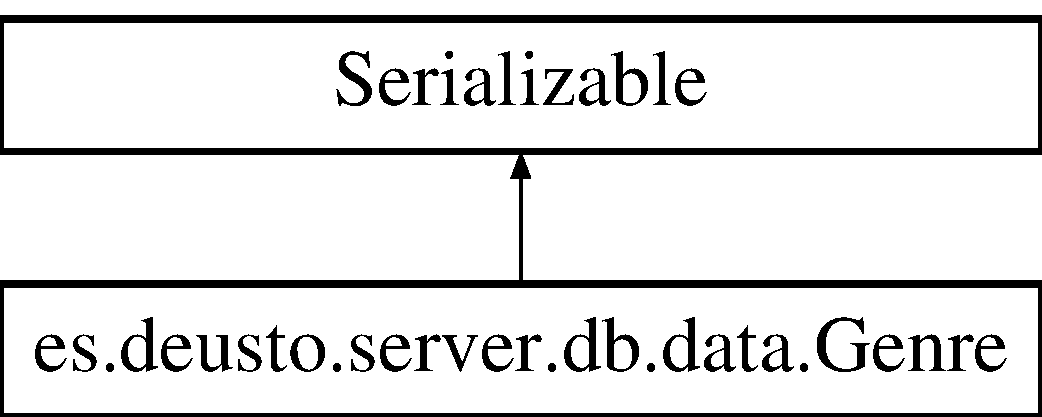
\includegraphics[height=2.000000cm]{classes_1_1deusto_1_1server_1_1db_1_1data_1_1_genre}
\end{center}
\end{figure}
\subsection*{Public Member Functions}
\begin{DoxyCompactItemize}
\item 
\hyperlink{classes_1_1deusto_1_1server_1_1db_1_1data_1_1_genre_a1fa29d6819400738c473a923bf03cbff}{Genre} (String name)
\item 
String \hyperlink{classes_1_1deusto_1_1server_1_1db_1_1data_1_1_genre_a9a68a612e2209b224801f1f7e0e9dcc9}{get\+Name} ()
\item 
void \hyperlink{classes_1_1deusto_1_1server_1_1db_1_1data_1_1_genre_a268b33c42da6c59b6688db28822e2369}{add\+Game} (\hyperlink{classes_1_1deusto_1_1server_1_1db_1_1data_1_1_game}{Game} game)
\item 
String \hyperlink{classes_1_1deusto_1_1server_1_1db_1_1data_1_1_genre_aeff531adb16e15f04a2f1a11b2b44af4}{to\+String} ()
\end{DoxyCompactItemize}


\subsection{Detailed Description}


Definition at line 14 of file Genre.\+java.



\subsection{Constructor \& Destructor Documentation}
\mbox{\Hypertarget{classes_1_1deusto_1_1server_1_1db_1_1data_1_1_genre_a1fa29d6819400738c473a923bf03cbff}\label{classes_1_1deusto_1_1server_1_1db_1_1data_1_1_genre_a1fa29d6819400738c473a923bf03cbff}} 
\index{es\+::deusto\+::server\+::db\+::data\+::\+Genre@{es\+::deusto\+::server\+::db\+::data\+::\+Genre}!Genre@{Genre}}
\index{Genre@{Genre}!es\+::deusto\+::server\+::db\+::data\+::\+Genre@{es\+::deusto\+::server\+::db\+::data\+::\+Genre}}
\subsubsection{\texorpdfstring{Genre()}{Genre()}}
{\footnotesize\ttfamily es.\+deusto.\+server.\+db.\+data.\+Genre.\+Genre (\begin{DoxyParamCaption}\item[{String}]{name }\end{DoxyParamCaption})}



Definition at line 24 of file Genre.\+java.



\subsection{Member Function Documentation}
\mbox{\Hypertarget{classes_1_1deusto_1_1server_1_1db_1_1data_1_1_genre_a268b33c42da6c59b6688db28822e2369}\label{classes_1_1deusto_1_1server_1_1db_1_1data_1_1_genre_a268b33c42da6c59b6688db28822e2369}} 
\index{es\+::deusto\+::server\+::db\+::data\+::\+Genre@{es\+::deusto\+::server\+::db\+::data\+::\+Genre}!add\+Game@{add\+Game}}
\index{add\+Game@{add\+Game}!es\+::deusto\+::server\+::db\+::data\+::\+Genre@{es\+::deusto\+::server\+::db\+::data\+::\+Genre}}
\subsubsection{\texorpdfstring{add\+Game()}{addGame()}}
{\footnotesize\ttfamily void es.\+deusto.\+server.\+db.\+data.\+Genre.\+add\+Game (\begin{DoxyParamCaption}\item[{\hyperlink{classes_1_1deusto_1_1server_1_1db_1_1data_1_1_game}{Game}}]{game }\end{DoxyParamCaption})}



Definition at line 33 of file Genre.\+java.

\mbox{\Hypertarget{classes_1_1deusto_1_1server_1_1db_1_1data_1_1_genre_a9a68a612e2209b224801f1f7e0e9dcc9}\label{classes_1_1deusto_1_1server_1_1db_1_1data_1_1_genre_a9a68a612e2209b224801f1f7e0e9dcc9}} 
\index{es\+::deusto\+::server\+::db\+::data\+::\+Genre@{es\+::deusto\+::server\+::db\+::data\+::\+Genre}!get\+Name@{get\+Name}}
\index{get\+Name@{get\+Name}!es\+::deusto\+::server\+::db\+::data\+::\+Genre@{es\+::deusto\+::server\+::db\+::data\+::\+Genre}}
\subsubsection{\texorpdfstring{get\+Name()}{getName()}}
{\footnotesize\ttfamily String es.\+deusto.\+server.\+db.\+data.\+Genre.\+get\+Name (\begin{DoxyParamCaption}{ }\end{DoxyParamCaption})}



Definition at line 29 of file Genre.\+java.

\mbox{\Hypertarget{classes_1_1deusto_1_1server_1_1db_1_1data_1_1_genre_aeff531adb16e15f04a2f1a11b2b44af4}\label{classes_1_1deusto_1_1server_1_1db_1_1data_1_1_genre_aeff531adb16e15f04a2f1a11b2b44af4}} 
\index{es\+::deusto\+::server\+::db\+::data\+::\+Genre@{es\+::deusto\+::server\+::db\+::data\+::\+Genre}!to\+String@{to\+String}}
\index{to\+String@{to\+String}!es\+::deusto\+::server\+::db\+::data\+::\+Genre@{es\+::deusto\+::server\+::db\+::data\+::\+Genre}}
\subsubsection{\texorpdfstring{to\+String()}{toString()}}
{\footnotesize\ttfamily String es.\+deusto.\+server.\+db.\+data.\+Genre.\+to\+String (\begin{DoxyParamCaption}{ }\end{DoxyParamCaption})}



Definition at line 38 of file Genre.\+java.



The documentation for this class was generated from the following file\+:\begin{DoxyCompactItemize}
\item 
C\+:/\+Users/\+Marta/\+S\+P\+Q09/\+Lurrun/src/main/java/es/deusto/server/db/data/\hyperlink{_genre_8java}{Genre.\+java}\end{DoxyCompactItemize}

\hypertarget{classes_1_1deusto_1_1client_1_1_g_u_i}{}\section{es.\+deusto.\+client.\+G\+UI Class Reference}
\label{classes_1_1deusto_1_1client_1_1_g_u_i}\index{es.\+deusto.\+client.\+G\+UI@{es.\+deusto.\+client.\+G\+UI}}
\subsection*{Public Member Functions}
\begin{DoxyCompactItemize}
\item 
void \hyperlink{classes_1_1deusto_1_1client_1_1_g_u_i_a71e596239fe49ac76586cf384aa95920}{ventana\+De\+Cliente} ()
\end{DoxyCompactItemize}


\subsection{Detailed Description}


Definition at line 3 of file G\+U\+I.\+java.



\subsection{Member Function Documentation}
\mbox{\Hypertarget{classes_1_1deusto_1_1client_1_1_g_u_i_a71e596239fe49ac76586cf384aa95920}\label{classes_1_1deusto_1_1client_1_1_g_u_i_a71e596239fe49ac76586cf384aa95920}} 
\index{es\+::deusto\+::client\+::\+G\+UI@{es\+::deusto\+::client\+::\+G\+UI}!ventana\+De\+Cliente@{ventana\+De\+Cliente}}
\index{ventana\+De\+Cliente@{ventana\+De\+Cliente}!es\+::deusto\+::client\+::\+G\+UI@{es\+::deusto\+::client\+::\+G\+UI}}
\subsubsection{\texorpdfstring{ventana\+De\+Cliente()}{ventanaDeCliente()}}
{\footnotesize\ttfamily void es.\+deusto.\+client.\+G\+U\+I.\+ventana\+De\+Cliente (\begin{DoxyParamCaption}{ }\end{DoxyParamCaption})}



Definition at line 6 of file G\+U\+I.\+java.



The documentation for this class was generated from the following file\+:\begin{DoxyCompactItemize}
\item 
src/main/java/es/deusto/client/\hyperlink{_g_u_i_8java}{G\+U\+I.\+java}\end{DoxyCompactItemize}

\hypertarget{interfacees_1_1deusto_1_1server_1_1db_1_1dao_1_1_i_d_a_o}{}\section{es.\+deusto.\+server.\+db.\+dao.\+I\+D\+AO Interface Reference}
\label{interfacees_1_1deusto_1_1server_1_1db_1_1dao_1_1_i_d_a_o}\index{es.\+deusto.\+server.\+db.\+dao.\+I\+D\+AO@{es.\+deusto.\+server.\+db.\+dao.\+I\+D\+AO}}
Inheritance diagram for es.\+deusto.\+server.\+db.\+dao.\+I\+D\+AO\+:\begin{figure}[H]
\begin{center}
\leavevmode
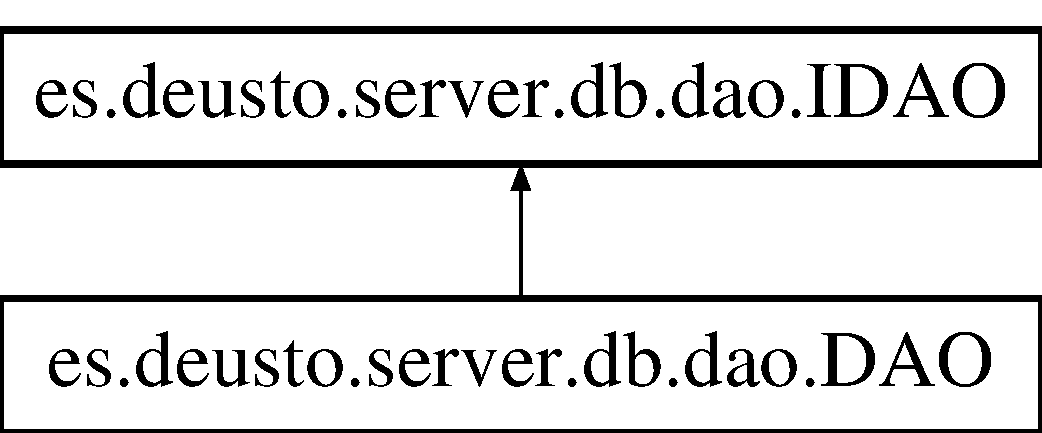
\includegraphics[height=2.000000cm]{interfacees_1_1deusto_1_1server_1_1db_1_1dao_1_1_i_d_a_o}
\end{center}
\end{figure}
\subsection*{Public Member Functions}
\begin{DoxyCompactItemize}
\item 
boolean \hyperlink{interfacees_1_1deusto_1_1server_1_1db_1_1dao_1_1_i_d_a_o_ab943216560f43595a852b406dcd394a4}{store\+User} (\hyperlink{classes_1_1deusto_1_1server_1_1db_1_1data_1_1_user}{User} u)
\item 
\hyperlink{classes_1_1deusto_1_1server_1_1db_1_1data_1_1_user}{User} \hyperlink{interfacees_1_1deusto_1_1server_1_1db_1_1dao_1_1_i_d_a_o_a19f9b0d0b6f5f80730d6d197deca7dfc}{retrieve\+User} (String login)
\item 
boolean \hyperlink{interfacees_1_1deusto_1_1server_1_1db_1_1dao_1_1_i_d_a_o_a790b00e2989b634c1bbb2c6620ff3583}{update\+User} (\hyperlink{classes_1_1deusto_1_1server_1_1db_1_1data_1_1_user}{User} u)
\item 
\hyperlink{classes_1_1deusto_1_1server_1_1db_1_1data_1_1_license}{License} \hyperlink{interfacees_1_1deusto_1_1server_1_1db_1_1dao_1_1_i_d_a_o_a6a3e25055d4a81c738d1bd73de6ef7da}{retrieve\+License} (String game\+Key)
\item 
boolean \hyperlink{interfacees_1_1deusto_1_1server_1_1db_1_1dao_1_1_i_d_a_o_a601329b95123948b10c3232687b11d5b}{update\+License} (\hyperlink{classes_1_1deusto_1_1server_1_1db_1_1data_1_1_license}{License} u)
\item 
boolean \hyperlink{interfacees_1_1deusto_1_1server_1_1db_1_1dao_1_1_i_d_a_o_ab38972c7c70c95b4c409fa7758ef2fc3}{store\+Game} (\hyperlink{classes_1_1deusto_1_1server_1_1db_1_1data_1_1_game}{Game} g)
\item 
\hyperlink{classes_1_1deusto_1_1server_1_1db_1_1data_1_1_game}{Game} \hyperlink{interfacees_1_1deusto_1_1server_1_1db_1_1dao_1_1_i_d_a_o_a30558c19c086ac0ffff6796a8ae208fb}{retrieve\+Game} (String name)
\item 
boolean \hyperlink{interfacees_1_1deusto_1_1server_1_1db_1_1dao_1_1_i_d_a_o_a3a3ca0456879e35349a937aac661ff3f}{update\+Game} (\hyperlink{classes_1_1deusto_1_1server_1_1db_1_1data_1_1_game}{Game} g)
\item 
\hyperlink{classes_1_1deusto_1_1server_1_1db_1_1data_1_1_company}{Company} \hyperlink{interfacees_1_1deusto_1_1server_1_1db_1_1dao_1_1_i_d_a_o_ad6fd7873e2191e887184e2261e34e3e5}{retrieve\+Company} (String name)
\item 
boolean \hyperlink{interfacees_1_1deusto_1_1server_1_1db_1_1dao_1_1_i_d_a_o_a2d4302c61abd557f5a84d0698afdb814}{update\+Company} (\hyperlink{classes_1_1deusto_1_1server_1_1db_1_1data_1_1_company}{Company} c)
\item 
\hyperlink{classes_1_1deusto_1_1server_1_1db_1_1data_1_1_genre}{Genre} \hyperlink{interfacees_1_1deusto_1_1server_1_1db_1_1dao_1_1_i_d_a_o_a8b15955637f9b81c57900761c6d03571}{retrieve\+Genre} (String name)
\item 
boolean \hyperlink{interfacees_1_1deusto_1_1server_1_1db_1_1dao_1_1_i_d_a_o_ae989ff2681d6afe8651a595340265c39}{update\+Genre} (\hyperlink{classes_1_1deusto_1_1server_1_1db_1_1data_1_1_genre}{Genre} g)
\item 
List$<$ \hyperlink{classes_1_1deusto_1_1server_1_1db_1_1data_1_1_game}{Game} $>$ \hyperlink{interfacees_1_1deusto_1_1server_1_1db_1_1dao_1_1_i_d_a_o_aebafef372cf3064b12d16fcb651b41ff}{get\+All\+Games} ()
\item 
List$<$ \hyperlink{classes_1_1deusto_1_1server_1_1db_1_1data_1_1_company}{Company} $>$ \hyperlink{interfacees_1_1deusto_1_1server_1_1db_1_1dao_1_1_i_d_a_o_ad83c37658f356cb69c1fa70f99416579}{get\+All\+Companies} ()
\item 
List$<$ \hyperlink{classes_1_1deusto_1_1server_1_1db_1_1data_1_1_genre}{Genre} $>$ \hyperlink{interfacees_1_1deusto_1_1server_1_1db_1_1dao_1_1_i_d_a_o_a96ad8de066318847a7828b12befe94f7}{get\+All\+Genres} ()
\item 
\hyperlink{classes_1_1deusto_1_1server_1_1db_1_1data_1_1_license}{License} \hyperlink{interfacees_1_1deusto_1_1server_1_1db_1_1dao_1_1_i_d_a_o_aef2783889a572e23bd57c5a2a955599a}{get\+First\+License} (String name)
\end{DoxyCompactItemize}


\subsection{Detailed Description}


Definition at line 6 of file I\+D\+A\+O.\+java.



\subsection{Member Function Documentation}
\mbox{\Hypertarget{interfacees_1_1deusto_1_1server_1_1db_1_1dao_1_1_i_d_a_o_ad83c37658f356cb69c1fa70f99416579}\label{interfacees_1_1deusto_1_1server_1_1db_1_1dao_1_1_i_d_a_o_ad83c37658f356cb69c1fa70f99416579}} 
\index{es\+::deusto\+::server\+::db\+::dao\+::\+I\+D\+AO@{es\+::deusto\+::server\+::db\+::dao\+::\+I\+D\+AO}!get\+All\+Companies@{get\+All\+Companies}}
\index{get\+All\+Companies@{get\+All\+Companies}!es\+::deusto\+::server\+::db\+::dao\+::\+I\+D\+AO@{es\+::deusto\+::server\+::db\+::dao\+::\+I\+D\+AO}}
\subsubsection{\texorpdfstring{get\+All\+Companies()}{getAllCompanies()}}
{\footnotesize\ttfamily List$<$\hyperlink{classes_1_1deusto_1_1server_1_1db_1_1data_1_1_company}{Company}$>$ es.\+deusto.\+server.\+db.\+dao.\+I\+D\+A\+O.\+get\+All\+Companies (\begin{DoxyParamCaption}{ }\end{DoxyParamCaption})}



Implemented in \hyperlink{classes_1_1deusto_1_1server_1_1db_1_1dao_1_1_d_a_o_ac564970c7e308393497e874655470aaa}{es.\+deusto.\+server.\+db.\+dao.\+D\+AO}.

\mbox{\Hypertarget{interfacees_1_1deusto_1_1server_1_1db_1_1dao_1_1_i_d_a_o_aebafef372cf3064b12d16fcb651b41ff}\label{interfacees_1_1deusto_1_1server_1_1db_1_1dao_1_1_i_d_a_o_aebafef372cf3064b12d16fcb651b41ff}} 
\index{es\+::deusto\+::server\+::db\+::dao\+::\+I\+D\+AO@{es\+::deusto\+::server\+::db\+::dao\+::\+I\+D\+AO}!get\+All\+Games@{get\+All\+Games}}
\index{get\+All\+Games@{get\+All\+Games}!es\+::deusto\+::server\+::db\+::dao\+::\+I\+D\+AO@{es\+::deusto\+::server\+::db\+::dao\+::\+I\+D\+AO}}
\subsubsection{\texorpdfstring{get\+All\+Games()}{getAllGames()}}
{\footnotesize\ttfamily List$<$\hyperlink{classes_1_1deusto_1_1server_1_1db_1_1data_1_1_game}{Game}$>$ es.\+deusto.\+server.\+db.\+dao.\+I\+D\+A\+O.\+get\+All\+Games (\begin{DoxyParamCaption}{ }\end{DoxyParamCaption})}



Implemented in \hyperlink{classes_1_1deusto_1_1server_1_1db_1_1dao_1_1_d_a_o_af49ed57bdac4dec48ab7616602d12df2}{es.\+deusto.\+server.\+db.\+dao.\+D\+AO}.

\mbox{\Hypertarget{interfacees_1_1deusto_1_1server_1_1db_1_1dao_1_1_i_d_a_o_a96ad8de066318847a7828b12befe94f7}\label{interfacees_1_1deusto_1_1server_1_1db_1_1dao_1_1_i_d_a_o_a96ad8de066318847a7828b12befe94f7}} 
\index{es\+::deusto\+::server\+::db\+::dao\+::\+I\+D\+AO@{es\+::deusto\+::server\+::db\+::dao\+::\+I\+D\+AO}!get\+All\+Genres@{get\+All\+Genres}}
\index{get\+All\+Genres@{get\+All\+Genres}!es\+::deusto\+::server\+::db\+::dao\+::\+I\+D\+AO@{es\+::deusto\+::server\+::db\+::dao\+::\+I\+D\+AO}}
\subsubsection{\texorpdfstring{get\+All\+Genres()}{getAllGenres()}}
{\footnotesize\ttfamily List$<$\hyperlink{classes_1_1deusto_1_1server_1_1db_1_1data_1_1_genre}{Genre}$>$ es.\+deusto.\+server.\+db.\+dao.\+I\+D\+A\+O.\+get\+All\+Genres (\begin{DoxyParamCaption}{ }\end{DoxyParamCaption})}



Implemented in \hyperlink{classes_1_1deusto_1_1server_1_1db_1_1dao_1_1_d_a_o_ac1cb7032ef21f53dead8347ef440f431}{es.\+deusto.\+server.\+db.\+dao.\+D\+AO}.

\mbox{\Hypertarget{interfacees_1_1deusto_1_1server_1_1db_1_1dao_1_1_i_d_a_o_aef2783889a572e23bd57c5a2a955599a}\label{interfacees_1_1deusto_1_1server_1_1db_1_1dao_1_1_i_d_a_o_aef2783889a572e23bd57c5a2a955599a}} 
\index{es\+::deusto\+::server\+::db\+::dao\+::\+I\+D\+AO@{es\+::deusto\+::server\+::db\+::dao\+::\+I\+D\+AO}!get\+First\+License@{get\+First\+License}}
\index{get\+First\+License@{get\+First\+License}!es\+::deusto\+::server\+::db\+::dao\+::\+I\+D\+AO@{es\+::deusto\+::server\+::db\+::dao\+::\+I\+D\+AO}}
\subsubsection{\texorpdfstring{get\+First\+License()}{getFirstLicense()}}
{\footnotesize\ttfamily \hyperlink{classes_1_1deusto_1_1server_1_1db_1_1data_1_1_license}{License} es.\+deusto.\+server.\+db.\+dao.\+I\+D\+A\+O.\+get\+First\+License (\begin{DoxyParamCaption}\item[{String}]{name }\end{DoxyParamCaption})}



Implemented in \hyperlink{classes_1_1deusto_1_1server_1_1db_1_1dao_1_1_d_a_o_a4a5a54059bac00ea6f3b6d21f2a31a02}{es.\+deusto.\+server.\+db.\+dao.\+D\+AO}.

\mbox{\Hypertarget{interfacees_1_1deusto_1_1server_1_1db_1_1dao_1_1_i_d_a_o_ad6fd7873e2191e887184e2261e34e3e5}\label{interfacees_1_1deusto_1_1server_1_1db_1_1dao_1_1_i_d_a_o_ad6fd7873e2191e887184e2261e34e3e5}} 
\index{es\+::deusto\+::server\+::db\+::dao\+::\+I\+D\+AO@{es\+::deusto\+::server\+::db\+::dao\+::\+I\+D\+AO}!retrieve\+Company@{retrieve\+Company}}
\index{retrieve\+Company@{retrieve\+Company}!es\+::deusto\+::server\+::db\+::dao\+::\+I\+D\+AO@{es\+::deusto\+::server\+::db\+::dao\+::\+I\+D\+AO}}
\subsubsection{\texorpdfstring{retrieve\+Company()}{retrieveCompany()}}
{\footnotesize\ttfamily \hyperlink{classes_1_1deusto_1_1server_1_1db_1_1data_1_1_company}{Company} es.\+deusto.\+server.\+db.\+dao.\+I\+D\+A\+O.\+retrieve\+Company (\begin{DoxyParamCaption}\item[{String}]{name }\end{DoxyParamCaption})}



Implemented in \hyperlink{classes_1_1deusto_1_1server_1_1db_1_1dao_1_1_d_a_o_aabd374b169473cfd6e1bdc4efc89b177}{es.\+deusto.\+server.\+db.\+dao.\+D\+AO}.

\mbox{\Hypertarget{interfacees_1_1deusto_1_1server_1_1db_1_1dao_1_1_i_d_a_o_a30558c19c086ac0ffff6796a8ae208fb}\label{interfacees_1_1deusto_1_1server_1_1db_1_1dao_1_1_i_d_a_o_a30558c19c086ac0ffff6796a8ae208fb}} 
\index{es\+::deusto\+::server\+::db\+::dao\+::\+I\+D\+AO@{es\+::deusto\+::server\+::db\+::dao\+::\+I\+D\+AO}!retrieve\+Game@{retrieve\+Game}}
\index{retrieve\+Game@{retrieve\+Game}!es\+::deusto\+::server\+::db\+::dao\+::\+I\+D\+AO@{es\+::deusto\+::server\+::db\+::dao\+::\+I\+D\+AO}}
\subsubsection{\texorpdfstring{retrieve\+Game()}{retrieveGame()}}
{\footnotesize\ttfamily \hyperlink{classes_1_1deusto_1_1server_1_1db_1_1data_1_1_game}{Game} es.\+deusto.\+server.\+db.\+dao.\+I\+D\+A\+O.\+retrieve\+Game (\begin{DoxyParamCaption}\item[{String}]{name }\end{DoxyParamCaption})}



Implemented in \hyperlink{classes_1_1deusto_1_1server_1_1db_1_1dao_1_1_d_a_o_ac94a91d3e5aeeb98fc12f087532b3506}{es.\+deusto.\+server.\+db.\+dao.\+D\+AO}.

\mbox{\Hypertarget{interfacees_1_1deusto_1_1server_1_1db_1_1dao_1_1_i_d_a_o_a8b15955637f9b81c57900761c6d03571}\label{interfacees_1_1deusto_1_1server_1_1db_1_1dao_1_1_i_d_a_o_a8b15955637f9b81c57900761c6d03571}} 
\index{es\+::deusto\+::server\+::db\+::dao\+::\+I\+D\+AO@{es\+::deusto\+::server\+::db\+::dao\+::\+I\+D\+AO}!retrieve\+Genre@{retrieve\+Genre}}
\index{retrieve\+Genre@{retrieve\+Genre}!es\+::deusto\+::server\+::db\+::dao\+::\+I\+D\+AO@{es\+::deusto\+::server\+::db\+::dao\+::\+I\+D\+AO}}
\subsubsection{\texorpdfstring{retrieve\+Genre()}{retrieveGenre()}}
{\footnotesize\ttfamily \hyperlink{classes_1_1deusto_1_1server_1_1db_1_1data_1_1_genre}{Genre} es.\+deusto.\+server.\+db.\+dao.\+I\+D\+A\+O.\+retrieve\+Genre (\begin{DoxyParamCaption}\item[{String}]{name }\end{DoxyParamCaption})}



Implemented in \hyperlink{classes_1_1deusto_1_1server_1_1db_1_1dao_1_1_d_a_o_a16b0af798fbb00cd29a505491c57e2cd}{es.\+deusto.\+server.\+db.\+dao.\+D\+AO}.

\mbox{\Hypertarget{interfacees_1_1deusto_1_1server_1_1db_1_1dao_1_1_i_d_a_o_a6a3e25055d4a81c738d1bd73de6ef7da}\label{interfacees_1_1deusto_1_1server_1_1db_1_1dao_1_1_i_d_a_o_a6a3e25055d4a81c738d1bd73de6ef7da}} 
\index{es\+::deusto\+::server\+::db\+::dao\+::\+I\+D\+AO@{es\+::deusto\+::server\+::db\+::dao\+::\+I\+D\+AO}!retrieve\+License@{retrieve\+License}}
\index{retrieve\+License@{retrieve\+License}!es\+::deusto\+::server\+::db\+::dao\+::\+I\+D\+AO@{es\+::deusto\+::server\+::db\+::dao\+::\+I\+D\+AO}}
\subsubsection{\texorpdfstring{retrieve\+License()}{retrieveLicense()}}
{\footnotesize\ttfamily \hyperlink{classes_1_1deusto_1_1server_1_1db_1_1data_1_1_license}{License} es.\+deusto.\+server.\+db.\+dao.\+I\+D\+A\+O.\+retrieve\+License (\begin{DoxyParamCaption}\item[{String}]{game\+Key }\end{DoxyParamCaption})}



Implemented in \hyperlink{classes_1_1deusto_1_1server_1_1db_1_1dao_1_1_d_a_o_a02fd634e6bd7a087b1476ab161af646f}{es.\+deusto.\+server.\+db.\+dao.\+D\+AO}.

\mbox{\Hypertarget{interfacees_1_1deusto_1_1server_1_1db_1_1dao_1_1_i_d_a_o_a19f9b0d0b6f5f80730d6d197deca7dfc}\label{interfacees_1_1deusto_1_1server_1_1db_1_1dao_1_1_i_d_a_o_a19f9b0d0b6f5f80730d6d197deca7dfc}} 
\index{es\+::deusto\+::server\+::db\+::dao\+::\+I\+D\+AO@{es\+::deusto\+::server\+::db\+::dao\+::\+I\+D\+AO}!retrieve\+User@{retrieve\+User}}
\index{retrieve\+User@{retrieve\+User}!es\+::deusto\+::server\+::db\+::dao\+::\+I\+D\+AO@{es\+::deusto\+::server\+::db\+::dao\+::\+I\+D\+AO}}
\subsubsection{\texorpdfstring{retrieve\+User()}{retrieveUser()}}
{\footnotesize\ttfamily \hyperlink{classes_1_1deusto_1_1server_1_1db_1_1data_1_1_user}{User} es.\+deusto.\+server.\+db.\+dao.\+I\+D\+A\+O.\+retrieve\+User (\begin{DoxyParamCaption}\item[{String}]{login }\end{DoxyParamCaption})}



Implemented in \hyperlink{classes_1_1deusto_1_1server_1_1db_1_1dao_1_1_d_a_o_a8c316b4c3bf246d00fb2b423a603ebe6}{es.\+deusto.\+server.\+db.\+dao.\+D\+AO}.

\mbox{\Hypertarget{interfacees_1_1deusto_1_1server_1_1db_1_1dao_1_1_i_d_a_o_ab38972c7c70c95b4c409fa7758ef2fc3}\label{interfacees_1_1deusto_1_1server_1_1db_1_1dao_1_1_i_d_a_o_ab38972c7c70c95b4c409fa7758ef2fc3}} 
\index{es\+::deusto\+::server\+::db\+::dao\+::\+I\+D\+AO@{es\+::deusto\+::server\+::db\+::dao\+::\+I\+D\+AO}!store\+Game@{store\+Game}}
\index{store\+Game@{store\+Game}!es\+::deusto\+::server\+::db\+::dao\+::\+I\+D\+AO@{es\+::deusto\+::server\+::db\+::dao\+::\+I\+D\+AO}}
\subsubsection{\texorpdfstring{store\+Game()}{storeGame()}}
{\footnotesize\ttfamily boolean es.\+deusto.\+server.\+db.\+dao.\+I\+D\+A\+O.\+store\+Game (\begin{DoxyParamCaption}\item[{\hyperlink{classes_1_1deusto_1_1server_1_1db_1_1data_1_1_game}{Game}}]{g }\end{DoxyParamCaption})}



Implemented in \hyperlink{classes_1_1deusto_1_1server_1_1db_1_1dao_1_1_d_a_o_a7484309d9b9b39c24cd7d0413a90c468}{es.\+deusto.\+server.\+db.\+dao.\+D\+AO}.

\mbox{\Hypertarget{interfacees_1_1deusto_1_1server_1_1db_1_1dao_1_1_i_d_a_o_ab943216560f43595a852b406dcd394a4}\label{interfacees_1_1deusto_1_1server_1_1db_1_1dao_1_1_i_d_a_o_ab943216560f43595a852b406dcd394a4}} 
\index{es\+::deusto\+::server\+::db\+::dao\+::\+I\+D\+AO@{es\+::deusto\+::server\+::db\+::dao\+::\+I\+D\+AO}!store\+User@{store\+User}}
\index{store\+User@{store\+User}!es\+::deusto\+::server\+::db\+::dao\+::\+I\+D\+AO@{es\+::deusto\+::server\+::db\+::dao\+::\+I\+D\+AO}}
\subsubsection{\texorpdfstring{store\+User()}{storeUser()}}
{\footnotesize\ttfamily boolean es.\+deusto.\+server.\+db.\+dao.\+I\+D\+A\+O.\+store\+User (\begin{DoxyParamCaption}\item[{\hyperlink{classes_1_1deusto_1_1server_1_1db_1_1data_1_1_user}{User}}]{u }\end{DoxyParamCaption})}



Implemented in \hyperlink{classes_1_1deusto_1_1server_1_1db_1_1dao_1_1_d_a_o_acb146e96959c340ef828ef8e36b4283c}{es.\+deusto.\+server.\+db.\+dao.\+D\+AO}.

\mbox{\Hypertarget{interfacees_1_1deusto_1_1server_1_1db_1_1dao_1_1_i_d_a_o_a2d4302c61abd557f5a84d0698afdb814}\label{interfacees_1_1deusto_1_1server_1_1db_1_1dao_1_1_i_d_a_o_a2d4302c61abd557f5a84d0698afdb814}} 
\index{es\+::deusto\+::server\+::db\+::dao\+::\+I\+D\+AO@{es\+::deusto\+::server\+::db\+::dao\+::\+I\+D\+AO}!update\+Company@{update\+Company}}
\index{update\+Company@{update\+Company}!es\+::deusto\+::server\+::db\+::dao\+::\+I\+D\+AO@{es\+::deusto\+::server\+::db\+::dao\+::\+I\+D\+AO}}
\subsubsection{\texorpdfstring{update\+Company()}{updateCompany()}}
{\footnotesize\ttfamily boolean es.\+deusto.\+server.\+db.\+dao.\+I\+D\+A\+O.\+update\+Company (\begin{DoxyParamCaption}\item[{\hyperlink{classes_1_1deusto_1_1server_1_1db_1_1data_1_1_company}{Company}}]{c }\end{DoxyParamCaption})}



Implemented in \hyperlink{classes_1_1deusto_1_1server_1_1db_1_1dao_1_1_d_a_o_a0748467c3346a5bcdcd79b508562b6dc}{es.\+deusto.\+server.\+db.\+dao.\+D\+AO}.

\mbox{\Hypertarget{interfacees_1_1deusto_1_1server_1_1db_1_1dao_1_1_i_d_a_o_a3a3ca0456879e35349a937aac661ff3f}\label{interfacees_1_1deusto_1_1server_1_1db_1_1dao_1_1_i_d_a_o_a3a3ca0456879e35349a937aac661ff3f}} 
\index{es\+::deusto\+::server\+::db\+::dao\+::\+I\+D\+AO@{es\+::deusto\+::server\+::db\+::dao\+::\+I\+D\+AO}!update\+Game@{update\+Game}}
\index{update\+Game@{update\+Game}!es\+::deusto\+::server\+::db\+::dao\+::\+I\+D\+AO@{es\+::deusto\+::server\+::db\+::dao\+::\+I\+D\+AO}}
\subsubsection{\texorpdfstring{update\+Game()}{updateGame()}}
{\footnotesize\ttfamily boolean es.\+deusto.\+server.\+db.\+dao.\+I\+D\+A\+O.\+update\+Game (\begin{DoxyParamCaption}\item[{\hyperlink{classes_1_1deusto_1_1server_1_1db_1_1data_1_1_game}{Game}}]{g }\end{DoxyParamCaption})}



Implemented in \hyperlink{classes_1_1deusto_1_1server_1_1db_1_1dao_1_1_d_a_o_ae7540010b43f96c5e50995a8376614e7}{es.\+deusto.\+server.\+db.\+dao.\+D\+AO}.

\mbox{\Hypertarget{interfacees_1_1deusto_1_1server_1_1db_1_1dao_1_1_i_d_a_o_ae989ff2681d6afe8651a595340265c39}\label{interfacees_1_1deusto_1_1server_1_1db_1_1dao_1_1_i_d_a_o_ae989ff2681d6afe8651a595340265c39}} 
\index{es\+::deusto\+::server\+::db\+::dao\+::\+I\+D\+AO@{es\+::deusto\+::server\+::db\+::dao\+::\+I\+D\+AO}!update\+Genre@{update\+Genre}}
\index{update\+Genre@{update\+Genre}!es\+::deusto\+::server\+::db\+::dao\+::\+I\+D\+AO@{es\+::deusto\+::server\+::db\+::dao\+::\+I\+D\+AO}}
\subsubsection{\texorpdfstring{update\+Genre()}{updateGenre()}}
{\footnotesize\ttfamily boolean es.\+deusto.\+server.\+db.\+dao.\+I\+D\+A\+O.\+update\+Genre (\begin{DoxyParamCaption}\item[{\hyperlink{classes_1_1deusto_1_1server_1_1db_1_1data_1_1_genre}{Genre}}]{g }\end{DoxyParamCaption})}



Implemented in \hyperlink{classes_1_1deusto_1_1server_1_1db_1_1dao_1_1_d_a_o_ae08384fb32fa6936c93f6292dbe02c7e}{es.\+deusto.\+server.\+db.\+dao.\+D\+AO}.

\mbox{\Hypertarget{interfacees_1_1deusto_1_1server_1_1db_1_1dao_1_1_i_d_a_o_a601329b95123948b10c3232687b11d5b}\label{interfacees_1_1deusto_1_1server_1_1db_1_1dao_1_1_i_d_a_o_a601329b95123948b10c3232687b11d5b}} 
\index{es\+::deusto\+::server\+::db\+::dao\+::\+I\+D\+AO@{es\+::deusto\+::server\+::db\+::dao\+::\+I\+D\+AO}!update\+License@{update\+License}}
\index{update\+License@{update\+License}!es\+::deusto\+::server\+::db\+::dao\+::\+I\+D\+AO@{es\+::deusto\+::server\+::db\+::dao\+::\+I\+D\+AO}}
\subsubsection{\texorpdfstring{update\+License()}{updateLicense()}}
{\footnotesize\ttfamily boolean es.\+deusto.\+server.\+db.\+dao.\+I\+D\+A\+O.\+update\+License (\begin{DoxyParamCaption}\item[{\hyperlink{classes_1_1deusto_1_1server_1_1db_1_1data_1_1_license}{License}}]{u }\end{DoxyParamCaption})}



Implemented in \hyperlink{classes_1_1deusto_1_1server_1_1db_1_1dao_1_1_d_a_o_a98774e8d93cdd4d8d104a197bd37d4e1}{es.\+deusto.\+server.\+db.\+dao.\+D\+AO}.

\mbox{\Hypertarget{interfacees_1_1deusto_1_1server_1_1db_1_1dao_1_1_i_d_a_o_a790b00e2989b634c1bbb2c6620ff3583}\label{interfacees_1_1deusto_1_1server_1_1db_1_1dao_1_1_i_d_a_o_a790b00e2989b634c1bbb2c6620ff3583}} 
\index{es\+::deusto\+::server\+::db\+::dao\+::\+I\+D\+AO@{es\+::deusto\+::server\+::db\+::dao\+::\+I\+D\+AO}!update\+User@{update\+User}}
\index{update\+User@{update\+User}!es\+::deusto\+::server\+::db\+::dao\+::\+I\+D\+AO@{es\+::deusto\+::server\+::db\+::dao\+::\+I\+D\+AO}}
\subsubsection{\texorpdfstring{update\+User()}{updateUser()}}
{\footnotesize\ttfamily boolean es.\+deusto.\+server.\+db.\+dao.\+I\+D\+A\+O.\+update\+User (\begin{DoxyParamCaption}\item[{\hyperlink{classes_1_1deusto_1_1server_1_1db_1_1data_1_1_user}{User}}]{u }\end{DoxyParamCaption})}



Implemented in \hyperlink{classes_1_1deusto_1_1server_1_1db_1_1dao_1_1_d_a_o_a7f6ed77294fe1f61cbebbea410cef6e0}{es.\+deusto.\+server.\+db.\+dao.\+D\+AO}.



The documentation for this interface was generated from the following file\+:\begin{DoxyCompactItemize}
\item 
C\+:/\+Users/\+Marta/\+S\+P\+Q09/\+Lurrun/src/main/java/es/deusto/server/db/dao/\hyperlink{_i_d_a_o_8java}{I\+D\+A\+O.\+java}\end{DoxyCompactItemize}

\hypertarget{interfacees_1_1deusto_1_1server_1_1db_1_1_i_d_b}{}\section{es.\+deusto.\+server.\+db.\+I\+DB Interface Reference}
\label{interfacees_1_1deusto_1_1server_1_1db_1_1_i_d_b}\index{es.\+deusto.\+server.\+db.\+I\+DB@{es.\+deusto.\+server.\+db.\+I\+DB}}
Inheritance diagram for es.\+deusto.\+server.\+db.\+I\+DB\+:\begin{figure}[H]
\begin{center}
\leavevmode
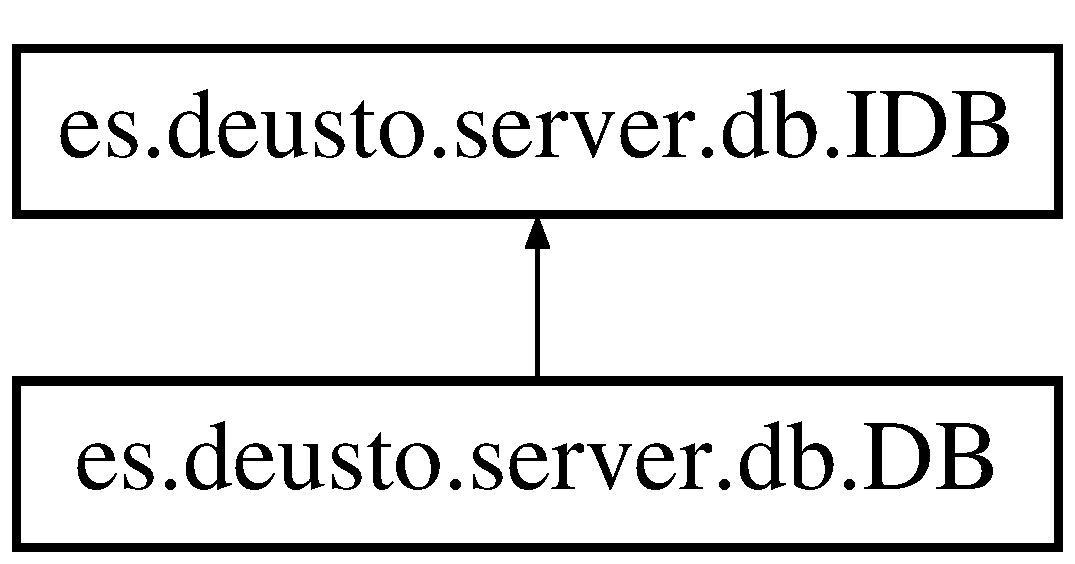
\includegraphics[height=2.000000cm]{interfacees_1_1deusto_1_1server_1_1db_1_1_i_d_b}
\end{center}
\end{figure}
\subsection*{Public Member Functions}
\begin{DoxyCompactItemize}
\item 
List$<$ \hyperlink{classes_1_1deusto_1_1server_1_1db_1_1data_1_1_game}{Game} $>$ \hyperlink{interfacees_1_1deusto_1_1server_1_1db_1_1_i_d_b_a76af81d4bb71c81490da92d67c5b6d03}{get\+All\+Games} ()
\item 
List$<$ \hyperlink{classes_1_1deusto_1_1server_1_1db_1_1data_1_1_user}{User} $>$ \hyperlink{interfacees_1_1deusto_1_1server_1_1db_1_1_i_d_b_ab2893cf6b112e1789b5a9e62f5156f6a}{get\+All\+Users} ()
\item 
List$<$ \hyperlink{classes_1_1deusto_1_1server_1_1db_1_1data_1_1_game}{Game} $>$ \hyperlink{interfacees_1_1deusto_1_1server_1_1db_1_1_i_d_b_ac5ef9780a640140576f9373f8b57631c}{get\+User\+Games} (String login)
\item 
boolean \hyperlink{interfacees_1_1deusto_1_1server_1_1db_1_1_i_d_b_ab1076d02bd6b4da29d0e99e1310048b6}{buy\+Game} (String login, String game)
\item 
boolean \hyperlink{interfacees_1_1deusto_1_1server_1_1db_1_1_i_d_b_ad9ecf628cb97ade7cb1b10fd1b3a18c4}{register\+User} (\hyperlink{classes_1_1deusto_1_1server_1_1db_1_1data_1_1_user}{User} u)
\item 
boolean \hyperlink{interfacees_1_1deusto_1_1server_1_1db_1_1_i_d_b_a645335b2cbfa27c0199783ff2f33559e}{add\+Game\+To\+Db} (\hyperlink{classes_1_1deusto_1_1server_1_1db_1_1data_1_1_game}{Game} g, \hyperlink{classes_1_1deusto_1_1server_1_1db_1_1data_1_1_genre}{Genre} gg, \hyperlink{classes_1_1deusto_1_1server_1_1db_1_1data_1_1_company}{Company} c)
\item 
boolean \hyperlink{interfacees_1_1deusto_1_1server_1_1db_1_1_i_d_b_ab2c9cbce259134d238e56eea5d0134c5}{add\+License\+To\+User} (\hyperlink{classes_1_1deusto_1_1server_1_1db_1_1data_1_1_user}{User} u, \hyperlink{classes_1_1deusto_1_1server_1_1db_1_1data_1_1_license}{License} l)
\item 
boolean \hyperlink{interfacees_1_1deusto_1_1server_1_1db_1_1_i_d_b_a6ca49e0ed9bd7826c4ee65cb5f0f583b}{add\+License\+To\+Game} (\hyperlink{classes_1_1deusto_1_1server_1_1db_1_1data_1_1_game}{Game} g, \hyperlink{classes_1_1deusto_1_1server_1_1db_1_1data_1_1_license}{License} l)
\item 
\hyperlink{classes_1_1deusto_1_1server_1_1db_1_1data_1_1_genre}{Genre} \hyperlink{interfacees_1_1deusto_1_1server_1_1db_1_1_i_d_b_a9023bdad77781d95fc2e556d1935f763}{show\+Genre} (String name)
\item 
\hyperlink{classes_1_1deusto_1_1server_1_1db_1_1data_1_1_game}{Game} \hyperlink{interfacees_1_1deusto_1_1server_1_1db_1_1_i_d_b_a572028cc62d36bebee977200b55eba8b}{show\+Game} (String name)
\item 
\hyperlink{classes_1_1deusto_1_1server_1_1db_1_1data_1_1_license}{License} \hyperlink{interfacees_1_1deusto_1_1server_1_1db_1_1_i_d_b_ad408b5a93077c152ceba270caa34fd0a}{show\+License} (String game\+Key)
\item 
\hyperlink{classes_1_1deusto_1_1server_1_1db_1_1data_1_1_company}{Company} \hyperlink{interfacees_1_1deusto_1_1server_1_1db_1_1_i_d_b_a1681e29b5fbe4377b19e67fa939b2782}{show\+Company} (String name)
\item 
\hyperlink{classes_1_1deusto_1_1server_1_1db_1_1data_1_1_user}{User} \hyperlink{interfacees_1_1deusto_1_1server_1_1db_1_1_i_d_b_aa2f6a5291fa8aa78d5a73b5878d17986}{show\+User} (String login)
\item 
\hyperlink{classes_1_1deusto_1_1server_1_1db_1_1data_1_1_game}{Game} \hyperlink{interfacees_1_1deusto_1_1server_1_1db_1_1_i_d_b_a0364013a2f73f89fd5f8c635d5c9405a}{show\+Game\+By\+Param} (String name)
\item 
\hyperlink{classes_1_1deusto_1_1server_1_1db_1_1data_1_1_company}{Company} \hyperlink{interfacees_1_1deusto_1_1server_1_1db_1_1_i_d_b_aed0409031510630d50085eca53aff113}{show\+Company\+By\+Param} (String name)
\item 
\hyperlink{classes_1_1deusto_1_1server_1_1db_1_1data_1_1_genre}{Genre} \hyperlink{interfacees_1_1deusto_1_1server_1_1db_1_1_i_d_b_a836faee771a447be79c36d7d4289c614}{show\+Genre\+By\+Param} (String name)
\end{DoxyCompactItemize}


\subsection{Detailed Description}


Definition at line 7 of file I\+D\+B.\+java.



\subsection{Member Function Documentation}
\mbox{\Hypertarget{interfacees_1_1deusto_1_1server_1_1db_1_1_i_d_b_a645335b2cbfa27c0199783ff2f33559e}\label{interfacees_1_1deusto_1_1server_1_1db_1_1_i_d_b_a645335b2cbfa27c0199783ff2f33559e}} 
\index{es\+::deusto\+::server\+::db\+::\+I\+DB@{es\+::deusto\+::server\+::db\+::\+I\+DB}!add\+Game\+To\+Db@{add\+Game\+To\+Db}}
\index{add\+Game\+To\+Db@{add\+Game\+To\+Db}!es\+::deusto\+::server\+::db\+::\+I\+DB@{es\+::deusto\+::server\+::db\+::\+I\+DB}}
\subsubsection{\texorpdfstring{add\+Game\+To\+Db()}{addGameToDb()}}
{\footnotesize\ttfamily boolean es.\+deusto.\+server.\+db.\+I\+D\+B.\+add\+Game\+To\+Db (\begin{DoxyParamCaption}\item[{\hyperlink{classes_1_1deusto_1_1server_1_1db_1_1data_1_1_game}{Game}}]{g,  }\item[{\hyperlink{classes_1_1deusto_1_1server_1_1db_1_1data_1_1_genre}{Genre}}]{gg,  }\item[{\hyperlink{classes_1_1deusto_1_1server_1_1db_1_1data_1_1_company}{Company}}]{c }\end{DoxyParamCaption})}



Implemented in \hyperlink{classes_1_1deusto_1_1server_1_1db_1_1_d_b_a376112d91f8e3018821fd9362f6598ae}{es.\+deusto.\+server.\+db.\+DB}.

\mbox{\Hypertarget{interfacees_1_1deusto_1_1server_1_1db_1_1_i_d_b_a6ca49e0ed9bd7826c4ee65cb5f0f583b}\label{interfacees_1_1deusto_1_1server_1_1db_1_1_i_d_b_a6ca49e0ed9bd7826c4ee65cb5f0f583b}} 
\index{es\+::deusto\+::server\+::db\+::\+I\+DB@{es\+::deusto\+::server\+::db\+::\+I\+DB}!add\+License\+To\+Game@{add\+License\+To\+Game}}
\index{add\+License\+To\+Game@{add\+License\+To\+Game}!es\+::deusto\+::server\+::db\+::\+I\+DB@{es\+::deusto\+::server\+::db\+::\+I\+DB}}
\subsubsection{\texorpdfstring{add\+License\+To\+Game()}{addLicenseToGame()}}
{\footnotesize\ttfamily boolean es.\+deusto.\+server.\+db.\+I\+D\+B.\+add\+License\+To\+Game (\begin{DoxyParamCaption}\item[{\hyperlink{classes_1_1deusto_1_1server_1_1db_1_1data_1_1_game}{Game}}]{g,  }\item[{\hyperlink{classes_1_1deusto_1_1server_1_1db_1_1data_1_1_license}{License}}]{l }\end{DoxyParamCaption})}



Implemented in \hyperlink{classes_1_1deusto_1_1server_1_1db_1_1_d_b_a5f4f68a9d2b7d6e8fbcc6e28136b92c8}{es.\+deusto.\+server.\+db.\+DB}.

\mbox{\Hypertarget{interfacees_1_1deusto_1_1server_1_1db_1_1_i_d_b_ab2c9cbce259134d238e56eea5d0134c5}\label{interfacees_1_1deusto_1_1server_1_1db_1_1_i_d_b_ab2c9cbce259134d238e56eea5d0134c5}} 
\index{es\+::deusto\+::server\+::db\+::\+I\+DB@{es\+::deusto\+::server\+::db\+::\+I\+DB}!add\+License\+To\+User@{add\+License\+To\+User}}
\index{add\+License\+To\+User@{add\+License\+To\+User}!es\+::deusto\+::server\+::db\+::\+I\+DB@{es\+::deusto\+::server\+::db\+::\+I\+DB}}
\subsubsection{\texorpdfstring{add\+License\+To\+User()}{addLicenseToUser()}}
{\footnotesize\ttfamily boolean es.\+deusto.\+server.\+db.\+I\+D\+B.\+add\+License\+To\+User (\begin{DoxyParamCaption}\item[{\hyperlink{classes_1_1deusto_1_1server_1_1db_1_1data_1_1_user}{User}}]{u,  }\item[{\hyperlink{classes_1_1deusto_1_1server_1_1db_1_1data_1_1_license}{License}}]{l }\end{DoxyParamCaption})}



Implemented in \hyperlink{classes_1_1deusto_1_1server_1_1db_1_1_d_b_a996d40d6b184ea0dfa3dcab05bc04757}{es.\+deusto.\+server.\+db.\+DB}.

\mbox{\Hypertarget{interfacees_1_1deusto_1_1server_1_1db_1_1_i_d_b_ab1076d02bd6b4da29d0e99e1310048b6}\label{interfacees_1_1deusto_1_1server_1_1db_1_1_i_d_b_ab1076d02bd6b4da29d0e99e1310048b6}} 
\index{es\+::deusto\+::server\+::db\+::\+I\+DB@{es\+::deusto\+::server\+::db\+::\+I\+DB}!buy\+Game@{buy\+Game}}
\index{buy\+Game@{buy\+Game}!es\+::deusto\+::server\+::db\+::\+I\+DB@{es\+::deusto\+::server\+::db\+::\+I\+DB}}
\subsubsection{\texorpdfstring{buy\+Game()}{buyGame()}}
{\footnotesize\ttfamily boolean es.\+deusto.\+server.\+db.\+I\+D\+B.\+buy\+Game (\begin{DoxyParamCaption}\item[{String}]{login,  }\item[{String}]{game }\end{DoxyParamCaption})}



Implemented in \hyperlink{classes_1_1deusto_1_1server_1_1db_1_1_d_b_a8aa2e7531181a31b54850ca6665f87c2}{es.\+deusto.\+server.\+db.\+DB}.

\mbox{\Hypertarget{interfacees_1_1deusto_1_1server_1_1db_1_1_i_d_b_a76af81d4bb71c81490da92d67c5b6d03}\label{interfacees_1_1deusto_1_1server_1_1db_1_1_i_d_b_a76af81d4bb71c81490da92d67c5b6d03}} 
\index{es\+::deusto\+::server\+::db\+::\+I\+DB@{es\+::deusto\+::server\+::db\+::\+I\+DB}!get\+All\+Games@{get\+All\+Games}}
\index{get\+All\+Games@{get\+All\+Games}!es\+::deusto\+::server\+::db\+::\+I\+DB@{es\+::deusto\+::server\+::db\+::\+I\+DB}}
\subsubsection{\texorpdfstring{get\+All\+Games()}{getAllGames()}}
{\footnotesize\ttfamily List$<$\hyperlink{classes_1_1deusto_1_1server_1_1db_1_1data_1_1_game}{Game}$>$ es.\+deusto.\+server.\+db.\+I\+D\+B.\+get\+All\+Games (\begin{DoxyParamCaption}{ }\end{DoxyParamCaption})}



Implemented in \hyperlink{classes_1_1deusto_1_1server_1_1db_1_1_d_b_ad878c1c58062596b5e1b582ed496bd11}{es.\+deusto.\+server.\+db.\+DB}.

\mbox{\Hypertarget{interfacees_1_1deusto_1_1server_1_1db_1_1_i_d_b_ab2893cf6b112e1789b5a9e62f5156f6a}\label{interfacees_1_1deusto_1_1server_1_1db_1_1_i_d_b_ab2893cf6b112e1789b5a9e62f5156f6a}} 
\index{es\+::deusto\+::server\+::db\+::\+I\+DB@{es\+::deusto\+::server\+::db\+::\+I\+DB}!get\+All\+Users@{get\+All\+Users}}
\index{get\+All\+Users@{get\+All\+Users}!es\+::deusto\+::server\+::db\+::\+I\+DB@{es\+::deusto\+::server\+::db\+::\+I\+DB}}
\subsubsection{\texorpdfstring{get\+All\+Users()}{getAllUsers()}}
{\footnotesize\ttfamily List$<$\hyperlink{classes_1_1deusto_1_1server_1_1db_1_1data_1_1_user}{User}$>$ es.\+deusto.\+server.\+db.\+I\+D\+B.\+get\+All\+Users (\begin{DoxyParamCaption}{ }\end{DoxyParamCaption})}



Implemented in \hyperlink{classes_1_1deusto_1_1server_1_1db_1_1_d_b_a245d98f8d670e29804a28d60daa7835b}{es.\+deusto.\+server.\+db.\+DB}.

\mbox{\Hypertarget{interfacees_1_1deusto_1_1server_1_1db_1_1_i_d_b_ac5ef9780a640140576f9373f8b57631c}\label{interfacees_1_1deusto_1_1server_1_1db_1_1_i_d_b_ac5ef9780a640140576f9373f8b57631c}} 
\index{es\+::deusto\+::server\+::db\+::\+I\+DB@{es\+::deusto\+::server\+::db\+::\+I\+DB}!get\+User\+Games@{get\+User\+Games}}
\index{get\+User\+Games@{get\+User\+Games}!es\+::deusto\+::server\+::db\+::\+I\+DB@{es\+::deusto\+::server\+::db\+::\+I\+DB}}
\subsubsection{\texorpdfstring{get\+User\+Games()}{getUserGames()}}
{\footnotesize\ttfamily List$<$\hyperlink{classes_1_1deusto_1_1server_1_1db_1_1data_1_1_game}{Game}$>$ es.\+deusto.\+server.\+db.\+I\+D\+B.\+get\+User\+Games (\begin{DoxyParamCaption}\item[{String}]{login }\end{DoxyParamCaption})}



Implemented in \hyperlink{classes_1_1deusto_1_1server_1_1db_1_1_d_b_a1c471589284782e7ff1190f2b6c2369e}{es.\+deusto.\+server.\+db.\+DB}.

\mbox{\Hypertarget{interfacees_1_1deusto_1_1server_1_1db_1_1_i_d_b_ad9ecf628cb97ade7cb1b10fd1b3a18c4}\label{interfacees_1_1deusto_1_1server_1_1db_1_1_i_d_b_ad9ecf628cb97ade7cb1b10fd1b3a18c4}} 
\index{es\+::deusto\+::server\+::db\+::\+I\+DB@{es\+::deusto\+::server\+::db\+::\+I\+DB}!register\+User@{register\+User}}
\index{register\+User@{register\+User}!es\+::deusto\+::server\+::db\+::\+I\+DB@{es\+::deusto\+::server\+::db\+::\+I\+DB}}
\subsubsection{\texorpdfstring{register\+User()}{registerUser()}}
{\footnotesize\ttfamily boolean es.\+deusto.\+server.\+db.\+I\+D\+B.\+register\+User (\begin{DoxyParamCaption}\item[{\hyperlink{classes_1_1deusto_1_1server_1_1db_1_1data_1_1_user}{User}}]{u }\end{DoxyParamCaption})}



Implemented in \hyperlink{classes_1_1deusto_1_1server_1_1db_1_1_d_b_a888f468b3fc2a05520fca9ac135823e3}{es.\+deusto.\+server.\+db.\+DB}.

\mbox{\Hypertarget{interfacees_1_1deusto_1_1server_1_1db_1_1_i_d_b_a1681e29b5fbe4377b19e67fa939b2782}\label{interfacees_1_1deusto_1_1server_1_1db_1_1_i_d_b_a1681e29b5fbe4377b19e67fa939b2782}} 
\index{es\+::deusto\+::server\+::db\+::\+I\+DB@{es\+::deusto\+::server\+::db\+::\+I\+DB}!show\+Company@{show\+Company}}
\index{show\+Company@{show\+Company}!es\+::deusto\+::server\+::db\+::\+I\+DB@{es\+::deusto\+::server\+::db\+::\+I\+DB}}
\subsubsection{\texorpdfstring{show\+Company()}{showCompany()}}
{\footnotesize\ttfamily \hyperlink{classes_1_1deusto_1_1server_1_1db_1_1data_1_1_company}{Company} es.\+deusto.\+server.\+db.\+I\+D\+B.\+show\+Company (\begin{DoxyParamCaption}\item[{String}]{name }\end{DoxyParamCaption})}



Implemented in \hyperlink{classes_1_1deusto_1_1server_1_1db_1_1_d_b_ab5edf3ae158bb0501a882b1d724cc2a8}{es.\+deusto.\+server.\+db.\+DB}.

\mbox{\Hypertarget{interfacees_1_1deusto_1_1server_1_1db_1_1_i_d_b_aed0409031510630d50085eca53aff113}\label{interfacees_1_1deusto_1_1server_1_1db_1_1_i_d_b_aed0409031510630d50085eca53aff113}} 
\index{es\+::deusto\+::server\+::db\+::\+I\+DB@{es\+::deusto\+::server\+::db\+::\+I\+DB}!show\+Company\+By\+Param@{show\+Company\+By\+Param}}
\index{show\+Company\+By\+Param@{show\+Company\+By\+Param}!es\+::deusto\+::server\+::db\+::\+I\+DB@{es\+::deusto\+::server\+::db\+::\+I\+DB}}
\subsubsection{\texorpdfstring{show\+Company\+By\+Param()}{showCompanyByParam()}}
{\footnotesize\ttfamily \hyperlink{classes_1_1deusto_1_1server_1_1db_1_1data_1_1_company}{Company} es.\+deusto.\+server.\+db.\+I\+D\+B.\+show\+Company\+By\+Param (\begin{DoxyParamCaption}\item[{String}]{name }\end{DoxyParamCaption})}



Implemented in \hyperlink{classes_1_1deusto_1_1server_1_1db_1_1_d_b_a777cd6a4714b8a2838bd2e719f05336f}{es.\+deusto.\+server.\+db.\+DB}.

\mbox{\Hypertarget{interfacees_1_1deusto_1_1server_1_1db_1_1_i_d_b_a572028cc62d36bebee977200b55eba8b}\label{interfacees_1_1deusto_1_1server_1_1db_1_1_i_d_b_a572028cc62d36bebee977200b55eba8b}} 
\index{es\+::deusto\+::server\+::db\+::\+I\+DB@{es\+::deusto\+::server\+::db\+::\+I\+DB}!show\+Game@{show\+Game}}
\index{show\+Game@{show\+Game}!es\+::deusto\+::server\+::db\+::\+I\+DB@{es\+::deusto\+::server\+::db\+::\+I\+DB}}
\subsubsection{\texorpdfstring{show\+Game()}{showGame()}}
{\footnotesize\ttfamily \hyperlink{classes_1_1deusto_1_1server_1_1db_1_1data_1_1_game}{Game} es.\+deusto.\+server.\+db.\+I\+D\+B.\+show\+Game (\begin{DoxyParamCaption}\item[{String}]{name }\end{DoxyParamCaption})}



Implemented in \hyperlink{classes_1_1deusto_1_1server_1_1db_1_1_d_b_adba76c20f2fc7ed01d486564d881a718}{es.\+deusto.\+server.\+db.\+DB}.

\mbox{\Hypertarget{interfacees_1_1deusto_1_1server_1_1db_1_1_i_d_b_a0364013a2f73f89fd5f8c635d5c9405a}\label{interfacees_1_1deusto_1_1server_1_1db_1_1_i_d_b_a0364013a2f73f89fd5f8c635d5c9405a}} 
\index{es\+::deusto\+::server\+::db\+::\+I\+DB@{es\+::deusto\+::server\+::db\+::\+I\+DB}!show\+Game\+By\+Param@{show\+Game\+By\+Param}}
\index{show\+Game\+By\+Param@{show\+Game\+By\+Param}!es\+::deusto\+::server\+::db\+::\+I\+DB@{es\+::deusto\+::server\+::db\+::\+I\+DB}}
\subsubsection{\texorpdfstring{show\+Game\+By\+Param()}{showGameByParam()}}
{\footnotesize\ttfamily \hyperlink{classes_1_1deusto_1_1server_1_1db_1_1data_1_1_game}{Game} es.\+deusto.\+server.\+db.\+I\+D\+B.\+show\+Game\+By\+Param (\begin{DoxyParamCaption}\item[{String}]{name }\end{DoxyParamCaption})}



Implemented in \hyperlink{classes_1_1deusto_1_1server_1_1db_1_1_d_b_a4fc9590d7e5643184ef89c3f03468e7e}{es.\+deusto.\+server.\+db.\+DB}.

\mbox{\Hypertarget{interfacees_1_1deusto_1_1server_1_1db_1_1_i_d_b_a9023bdad77781d95fc2e556d1935f763}\label{interfacees_1_1deusto_1_1server_1_1db_1_1_i_d_b_a9023bdad77781d95fc2e556d1935f763}} 
\index{es\+::deusto\+::server\+::db\+::\+I\+DB@{es\+::deusto\+::server\+::db\+::\+I\+DB}!show\+Genre@{show\+Genre}}
\index{show\+Genre@{show\+Genre}!es\+::deusto\+::server\+::db\+::\+I\+DB@{es\+::deusto\+::server\+::db\+::\+I\+DB}}
\subsubsection{\texorpdfstring{show\+Genre()}{showGenre()}}
{\footnotesize\ttfamily \hyperlink{classes_1_1deusto_1_1server_1_1db_1_1data_1_1_genre}{Genre} es.\+deusto.\+server.\+db.\+I\+D\+B.\+show\+Genre (\begin{DoxyParamCaption}\item[{String}]{name }\end{DoxyParamCaption})}



Implemented in \hyperlink{classes_1_1deusto_1_1server_1_1db_1_1_d_b_a207ddeb183db925dc20f095033aa4d94}{es.\+deusto.\+server.\+db.\+DB}.

\mbox{\Hypertarget{interfacees_1_1deusto_1_1server_1_1db_1_1_i_d_b_a836faee771a447be79c36d7d4289c614}\label{interfacees_1_1deusto_1_1server_1_1db_1_1_i_d_b_a836faee771a447be79c36d7d4289c614}} 
\index{es\+::deusto\+::server\+::db\+::\+I\+DB@{es\+::deusto\+::server\+::db\+::\+I\+DB}!show\+Genre\+By\+Param@{show\+Genre\+By\+Param}}
\index{show\+Genre\+By\+Param@{show\+Genre\+By\+Param}!es\+::deusto\+::server\+::db\+::\+I\+DB@{es\+::deusto\+::server\+::db\+::\+I\+DB}}
\subsubsection{\texorpdfstring{show\+Genre\+By\+Param()}{showGenreByParam()}}
{\footnotesize\ttfamily \hyperlink{classes_1_1deusto_1_1server_1_1db_1_1data_1_1_genre}{Genre} es.\+deusto.\+server.\+db.\+I\+D\+B.\+show\+Genre\+By\+Param (\begin{DoxyParamCaption}\item[{String}]{name }\end{DoxyParamCaption})}



Implemented in \hyperlink{classes_1_1deusto_1_1server_1_1db_1_1_d_b_ad3da93de99d7123529260d5dd966f178}{es.\+deusto.\+server.\+db.\+DB}.

\mbox{\Hypertarget{interfacees_1_1deusto_1_1server_1_1db_1_1_i_d_b_ad408b5a93077c152ceba270caa34fd0a}\label{interfacees_1_1deusto_1_1server_1_1db_1_1_i_d_b_ad408b5a93077c152ceba270caa34fd0a}} 
\index{es\+::deusto\+::server\+::db\+::\+I\+DB@{es\+::deusto\+::server\+::db\+::\+I\+DB}!show\+License@{show\+License}}
\index{show\+License@{show\+License}!es\+::deusto\+::server\+::db\+::\+I\+DB@{es\+::deusto\+::server\+::db\+::\+I\+DB}}
\subsubsection{\texorpdfstring{show\+License()}{showLicense()}}
{\footnotesize\ttfamily \hyperlink{classes_1_1deusto_1_1server_1_1db_1_1data_1_1_license}{License} es.\+deusto.\+server.\+db.\+I\+D\+B.\+show\+License (\begin{DoxyParamCaption}\item[{String}]{game\+Key }\end{DoxyParamCaption})}



Implemented in \hyperlink{classes_1_1deusto_1_1server_1_1db_1_1_d_b_add49bccfecff6217efd34b4656572ed6}{es.\+deusto.\+server.\+db.\+DB}.

\mbox{\Hypertarget{interfacees_1_1deusto_1_1server_1_1db_1_1_i_d_b_aa2f6a5291fa8aa78d5a73b5878d17986}\label{interfacees_1_1deusto_1_1server_1_1db_1_1_i_d_b_aa2f6a5291fa8aa78d5a73b5878d17986}} 
\index{es\+::deusto\+::server\+::db\+::\+I\+DB@{es\+::deusto\+::server\+::db\+::\+I\+DB}!show\+User@{show\+User}}
\index{show\+User@{show\+User}!es\+::deusto\+::server\+::db\+::\+I\+DB@{es\+::deusto\+::server\+::db\+::\+I\+DB}}
\subsubsection{\texorpdfstring{show\+User()}{showUser()}}
{\footnotesize\ttfamily \hyperlink{classes_1_1deusto_1_1server_1_1db_1_1data_1_1_user}{User} es.\+deusto.\+server.\+db.\+I\+D\+B.\+show\+User (\begin{DoxyParamCaption}\item[{String}]{login }\end{DoxyParamCaption})}



Implemented in \hyperlink{classes_1_1deusto_1_1server_1_1db_1_1_d_b_ac85523faea523033439a932bbcab2c7e}{es.\+deusto.\+server.\+db.\+DB}.



The documentation for this interface was generated from the following file\+:\begin{DoxyCompactItemize}
\item 
C\+:/\+Users/\+Carazo\+\_\+laptop/git/\+S\+P\+Q09/\+Lurrun/src/main/java/es/deusto/server/db/\hyperlink{_i_d_b_8java}{I\+D\+B.\+java}\end{DoxyCompactItemize}

\hypertarget{interfacees_1_1deusto_1_1server_1_1remote_1_1_i_remote}{}\section{es.\+deusto.\+server.\+remote.\+I\+Remote Interface Reference}
\label{interfacees_1_1deusto_1_1server_1_1remote_1_1_i_remote}\index{es.\+deusto.\+server.\+remote.\+I\+Remote@{es.\+deusto.\+server.\+remote.\+I\+Remote}}
Inheritance diagram for es.\+deusto.\+server.\+remote.\+I\+Remote\+:\begin{figure}[H]
\begin{center}
\leavevmode
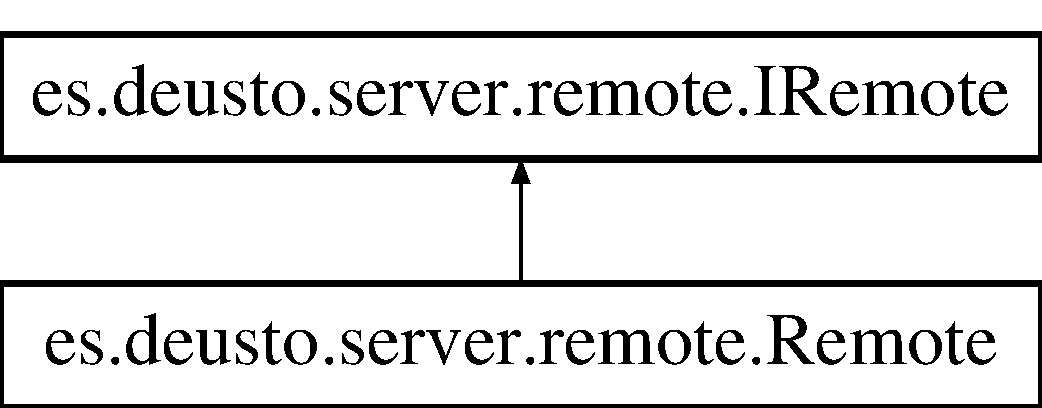
\includegraphics[height=2.000000cm]{interfacees_1_1deusto_1_1server_1_1remote_1_1_i_remote}
\end{center}
\end{figure}
\subsection*{Public Member Functions}
\begin{DoxyCompactItemize}
\item 
boolean \hyperlink{interfacees_1_1deusto_1_1server_1_1remote_1_1_i_remote_aea9a185d69da02d134443a3802a20b32}{register\+User} (String login, String password)  throws Remote\+Exception
\item 
boolean \hyperlink{interfacees_1_1deusto_1_1server_1_1remote_1_1_i_remote_a19acdbd6565b0f00cbe860a3316071ad}{login\+User} (String login, String password)  throws Remote\+Exception
\item 
List$<$ \hyperlink{classes_1_1deusto_1_1server_1_1db_1_1data_1_1_game}{Game} $>$ \hyperlink{interfacees_1_1deusto_1_1server_1_1remote_1_1_i_remote_a091249da31b567c1be29e07085d3ff18}{show\+Games\+In\+Store} ()  throws Remote\+Exception
\item 
List$<$ \hyperlink{classes_1_1deusto_1_1server_1_1db_1_1data_1_1_game}{Game} $>$ \hyperlink{interfacees_1_1deusto_1_1server_1_1remote_1_1_i_remote_aaaf6af5906c81cbd7b3b190a70ead98b}{show\+Owned\+Games} (String username)  throws Remote\+Exception
\item 
boolean \hyperlink{interfacees_1_1deusto_1_1server_1_1remote_1_1_i_remote_ad2e6ee616bdc780b4057e63bf2ae8be7}{buy\+Game} (String username, String name)  throws Remote\+Exception
\item 
double \hyperlink{interfacees_1_1deusto_1_1server_1_1remote_1_1_i_remote_a53305dbc72d910c932e66e2c27c5e1bb}{get\+User\+Wallet} (String login)  throws Remote\+Exception
\item 
boolean \hyperlink{interfacees_1_1deusto_1_1server_1_1remote_1_1_i_remote_a488f8b57271876e219af445345428d73}{is\+Super\+User} (String login)  throws Remote\+Exception
\item 
boolean \hyperlink{interfacees_1_1deusto_1_1server_1_1remote_1_1_i_remote_a991909db4d26d5be67bb3e0bcb501c7e}{add\+Game} (String g\+Name, double price, double disc, String gg, String c)  throws Remote\+Exception
\item 
String \mbox{[}$\,$\mbox{]} \hyperlink{interfacees_1_1deusto_1_1server_1_1remote_1_1_i_remote_a43ab8347d64e5d49093e607029f2598b}{get\+All\+Companies} ()  throws Remote\+Exception
\item 
String \mbox{[}$\,$\mbox{]} \hyperlink{interfacees_1_1deusto_1_1server_1_1remote_1_1_i_remote_a7c3721ee532d20aa65b892b55f157b21}{get\+All\+Genres} ()  throws Remote\+Exception
\end{DoxyCompactItemize}


\subsection{Detailed Description}


Definition at line 9 of file I\+Remote.\+java.



\subsection{Member Function Documentation}
\mbox{\Hypertarget{interfacees_1_1deusto_1_1server_1_1remote_1_1_i_remote_a991909db4d26d5be67bb3e0bcb501c7e}\label{interfacees_1_1deusto_1_1server_1_1remote_1_1_i_remote_a991909db4d26d5be67bb3e0bcb501c7e}} 
\index{es\+::deusto\+::server\+::remote\+::\+I\+Remote@{es\+::deusto\+::server\+::remote\+::\+I\+Remote}!add\+Game@{add\+Game}}
\index{add\+Game@{add\+Game}!es\+::deusto\+::server\+::remote\+::\+I\+Remote@{es\+::deusto\+::server\+::remote\+::\+I\+Remote}}
\subsubsection{\texorpdfstring{add\+Game()}{addGame()}}
{\footnotesize\ttfamily boolean es.\+deusto.\+server.\+remote.\+I\+Remote.\+add\+Game (\begin{DoxyParamCaption}\item[{String}]{g\+Name,  }\item[{double}]{price,  }\item[{double}]{disc,  }\item[{String}]{gg,  }\item[{String}]{c }\end{DoxyParamCaption}) throws Remote\+Exception}



Implemented in \hyperlink{classes_1_1deusto_1_1server_1_1remote_1_1_remote_a81c61e602f9419408e0069b51bc1e740}{es.\+deusto.\+server.\+remote.\+Remote}.

\mbox{\Hypertarget{interfacees_1_1deusto_1_1server_1_1remote_1_1_i_remote_ad2e6ee616bdc780b4057e63bf2ae8be7}\label{interfacees_1_1deusto_1_1server_1_1remote_1_1_i_remote_ad2e6ee616bdc780b4057e63bf2ae8be7}} 
\index{es\+::deusto\+::server\+::remote\+::\+I\+Remote@{es\+::deusto\+::server\+::remote\+::\+I\+Remote}!buy\+Game@{buy\+Game}}
\index{buy\+Game@{buy\+Game}!es\+::deusto\+::server\+::remote\+::\+I\+Remote@{es\+::deusto\+::server\+::remote\+::\+I\+Remote}}
\subsubsection{\texorpdfstring{buy\+Game()}{buyGame()}}
{\footnotesize\ttfamily boolean es.\+deusto.\+server.\+remote.\+I\+Remote.\+buy\+Game (\begin{DoxyParamCaption}\item[{String}]{username,  }\item[{String}]{name }\end{DoxyParamCaption}) throws Remote\+Exception}



Implemented in \hyperlink{classes_1_1deusto_1_1server_1_1remote_1_1_remote_ad9f8ad426b1162504b7b39eb1c86d2a3}{es.\+deusto.\+server.\+remote.\+Remote}.

\mbox{\Hypertarget{interfacees_1_1deusto_1_1server_1_1remote_1_1_i_remote_a43ab8347d64e5d49093e607029f2598b}\label{interfacees_1_1deusto_1_1server_1_1remote_1_1_i_remote_a43ab8347d64e5d49093e607029f2598b}} 
\index{es\+::deusto\+::server\+::remote\+::\+I\+Remote@{es\+::deusto\+::server\+::remote\+::\+I\+Remote}!get\+All\+Companies@{get\+All\+Companies}}
\index{get\+All\+Companies@{get\+All\+Companies}!es\+::deusto\+::server\+::remote\+::\+I\+Remote@{es\+::deusto\+::server\+::remote\+::\+I\+Remote}}
\subsubsection{\texorpdfstring{get\+All\+Companies()}{getAllCompanies()}}
{\footnotesize\ttfamily String \mbox{[}$\,$\mbox{]} es.\+deusto.\+server.\+remote.\+I\+Remote.\+get\+All\+Companies (\begin{DoxyParamCaption}{ }\end{DoxyParamCaption}) throws Remote\+Exception}



Implemented in \hyperlink{classes_1_1deusto_1_1server_1_1remote_1_1_remote_ab8595d6689604ef57f2d01309936ccd2}{es.\+deusto.\+server.\+remote.\+Remote}.

\mbox{\Hypertarget{interfacees_1_1deusto_1_1server_1_1remote_1_1_i_remote_a7c3721ee532d20aa65b892b55f157b21}\label{interfacees_1_1deusto_1_1server_1_1remote_1_1_i_remote_a7c3721ee532d20aa65b892b55f157b21}} 
\index{es\+::deusto\+::server\+::remote\+::\+I\+Remote@{es\+::deusto\+::server\+::remote\+::\+I\+Remote}!get\+All\+Genres@{get\+All\+Genres}}
\index{get\+All\+Genres@{get\+All\+Genres}!es\+::deusto\+::server\+::remote\+::\+I\+Remote@{es\+::deusto\+::server\+::remote\+::\+I\+Remote}}
\subsubsection{\texorpdfstring{get\+All\+Genres()}{getAllGenres()}}
{\footnotesize\ttfamily String \mbox{[}$\,$\mbox{]} es.\+deusto.\+server.\+remote.\+I\+Remote.\+get\+All\+Genres (\begin{DoxyParamCaption}{ }\end{DoxyParamCaption}) throws Remote\+Exception}



Implemented in \hyperlink{classes_1_1deusto_1_1server_1_1remote_1_1_remote_a89ce5459e2ebe375dc534e59eda91b74}{es.\+deusto.\+server.\+remote.\+Remote}.

\mbox{\Hypertarget{interfacees_1_1deusto_1_1server_1_1remote_1_1_i_remote_a53305dbc72d910c932e66e2c27c5e1bb}\label{interfacees_1_1deusto_1_1server_1_1remote_1_1_i_remote_a53305dbc72d910c932e66e2c27c5e1bb}} 
\index{es\+::deusto\+::server\+::remote\+::\+I\+Remote@{es\+::deusto\+::server\+::remote\+::\+I\+Remote}!get\+User\+Wallet@{get\+User\+Wallet}}
\index{get\+User\+Wallet@{get\+User\+Wallet}!es\+::deusto\+::server\+::remote\+::\+I\+Remote@{es\+::deusto\+::server\+::remote\+::\+I\+Remote}}
\subsubsection{\texorpdfstring{get\+User\+Wallet()}{getUserWallet()}}
{\footnotesize\ttfamily double es.\+deusto.\+server.\+remote.\+I\+Remote.\+get\+User\+Wallet (\begin{DoxyParamCaption}\item[{String}]{login }\end{DoxyParamCaption}) throws Remote\+Exception}



Implemented in \hyperlink{classes_1_1deusto_1_1server_1_1remote_1_1_remote_af7cc190cccf69cda838a6d9805c5c2f5}{es.\+deusto.\+server.\+remote.\+Remote}.

\mbox{\Hypertarget{interfacees_1_1deusto_1_1server_1_1remote_1_1_i_remote_a488f8b57271876e219af445345428d73}\label{interfacees_1_1deusto_1_1server_1_1remote_1_1_i_remote_a488f8b57271876e219af445345428d73}} 
\index{es\+::deusto\+::server\+::remote\+::\+I\+Remote@{es\+::deusto\+::server\+::remote\+::\+I\+Remote}!is\+Super\+User@{is\+Super\+User}}
\index{is\+Super\+User@{is\+Super\+User}!es\+::deusto\+::server\+::remote\+::\+I\+Remote@{es\+::deusto\+::server\+::remote\+::\+I\+Remote}}
\subsubsection{\texorpdfstring{is\+Super\+User()}{isSuperUser()}}
{\footnotesize\ttfamily boolean es.\+deusto.\+server.\+remote.\+I\+Remote.\+is\+Super\+User (\begin{DoxyParamCaption}\item[{String}]{login }\end{DoxyParamCaption}) throws Remote\+Exception}



Implemented in \hyperlink{classes_1_1deusto_1_1server_1_1remote_1_1_remote_ac7d2e76813b61b5a9fcf33d89b6e08c4}{es.\+deusto.\+server.\+remote.\+Remote}.

\mbox{\Hypertarget{interfacees_1_1deusto_1_1server_1_1remote_1_1_i_remote_a19acdbd6565b0f00cbe860a3316071ad}\label{interfacees_1_1deusto_1_1server_1_1remote_1_1_i_remote_a19acdbd6565b0f00cbe860a3316071ad}} 
\index{es\+::deusto\+::server\+::remote\+::\+I\+Remote@{es\+::deusto\+::server\+::remote\+::\+I\+Remote}!login\+User@{login\+User}}
\index{login\+User@{login\+User}!es\+::deusto\+::server\+::remote\+::\+I\+Remote@{es\+::deusto\+::server\+::remote\+::\+I\+Remote}}
\subsubsection{\texorpdfstring{login\+User()}{loginUser()}}
{\footnotesize\ttfamily boolean es.\+deusto.\+server.\+remote.\+I\+Remote.\+login\+User (\begin{DoxyParamCaption}\item[{String}]{login,  }\item[{String}]{password }\end{DoxyParamCaption}) throws Remote\+Exception}



Implemented in \hyperlink{classes_1_1deusto_1_1server_1_1remote_1_1_remote_a1c8e0153dd9b3f6d5499eb6d01e48bbe}{es.\+deusto.\+server.\+remote.\+Remote}.

\mbox{\Hypertarget{interfacees_1_1deusto_1_1server_1_1remote_1_1_i_remote_aea9a185d69da02d134443a3802a20b32}\label{interfacees_1_1deusto_1_1server_1_1remote_1_1_i_remote_aea9a185d69da02d134443a3802a20b32}} 
\index{es\+::deusto\+::server\+::remote\+::\+I\+Remote@{es\+::deusto\+::server\+::remote\+::\+I\+Remote}!register\+User@{register\+User}}
\index{register\+User@{register\+User}!es\+::deusto\+::server\+::remote\+::\+I\+Remote@{es\+::deusto\+::server\+::remote\+::\+I\+Remote}}
\subsubsection{\texorpdfstring{register\+User()}{registerUser()}}
{\footnotesize\ttfamily boolean es.\+deusto.\+server.\+remote.\+I\+Remote.\+register\+User (\begin{DoxyParamCaption}\item[{String}]{login,  }\item[{String}]{password }\end{DoxyParamCaption}) throws Remote\+Exception}



Implemented in \hyperlink{classes_1_1deusto_1_1server_1_1remote_1_1_remote_a4b013f75d23e2c9f0dbca2d3bb467f6a}{es.\+deusto.\+server.\+remote.\+Remote}.

\mbox{\Hypertarget{interfacees_1_1deusto_1_1server_1_1remote_1_1_i_remote_a091249da31b567c1be29e07085d3ff18}\label{interfacees_1_1deusto_1_1server_1_1remote_1_1_i_remote_a091249da31b567c1be29e07085d3ff18}} 
\index{es\+::deusto\+::server\+::remote\+::\+I\+Remote@{es\+::deusto\+::server\+::remote\+::\+I\+Remote}!show\+Games\+In\+Store@{show\+Games\+In\+Store}}
\index{show\+Games\+In\+Store@{show\+Games\+In\+Store}!es\+::deusto\+::server\+::remote\+::\+I\+Remote@{es\+::deusto\+::server\+::remote\+::\+I\+Remote}}
\subsubsection{\texorpdfstring{show\+Games\+In\+Store()}{showGamesInStore()}}
{\footnotesize\ttfamily List$<$\hyperlink{classes_1_1deusto_1_1server_1_1db_1_1data_1_1_game}{Game}$>$ es.\+deusto.\+server.\+remote.\+I\+Remote.\+show\+Games\+In\+Store (\begin{DoxyParamCaption}{ }\end{DoxyParamCaption}) throws Remote\+Exception}



Implemented in \hyperlink{classes_1_1deusto_1_1server_1_1remote_1_1_remote_ae40a5882d6b3ef3d5928d87dafeb15fa}{es.\+deusto.\+server.\+remote.\+Remote}.

\mbox{\Hypertarget{interfacees_1_1deusto_1_1server_1_1remote_1_1_i_remote_aaaf6af5906c81cbd7b3b190a70ead98b}\label{interfacees_1_1deusto_1_1server_1_1remote_1_1_i_remote_aaaf6af5906c81cbd7b3b190a70ead98b}} 
\index{es\+::deusto\+::server\+::remote\+::\+I\+Remote@{es\+::deusto\+::server\+::remote\+::\+I\+Remote}!show\+Owned\+Games@{show\+Owned\+Games}}
\index{show\+Owned\+Games@{show\+Owned\+Games}!es\+::deusto\+::server\+::remote\+::\+I\+Remote@{es\+::deusto\+::server\+::remote\+::\+I\+Remote}}
\subsubsection{\texorpdfstring{show\+Owned\+Games()}{showOwnedGames()}}
{\footnotesize\ttfamily List$<$\hyperlink{classes_1_1deusto_1_1server_1_1db_1_1data_1_1_game}{Game}$>$ es.\+deusto.\+server.\+remote.\+I\+Remote.\+show\+Owned\+Games (\begin{DoxyParamCaption}\item[{String}]{username }\end{DoxyParamCaption}) throws Remote\+Exception}



Implemented in \hyperlink{classes_1_1deusto_1_1server_1_1remote_1_1_remote_a73569877f9317fc48a4e134977baa304}{es.\+deusto.\+server.\+remote.\+Remote}.



The documentation for this interface was generated from the following file\+:\begin{DoxyCompactItemize}
\item 
C\+:/\+Users/\+Marta/\+S\+P\+Q09/\+Lurrun/src/main/java/es/deusto/server/remote/\hyperlink{_i_remote_8java}{I\+Remote.\+java}\end{DoxyCompactItemize}

\hypertarget{classes_1_1deusto_1_1server_1_1db_1_1data_1_1_license}{}\section{es.\+deusto.\+server.\+db.\+data.\+License Class Reference}
\label{classes_1_1deusto_1_1server_1_1db_1_1data_1_1_license}\index{es.\+deusto.\+server.\+db.\+data.\+License@{es.\+deusto.\+server.\+db.\+data.\+License}}
Inheritance diagram for es.\+deusto.\+server.\+db.\+data.\+License\+:\begin{figure}[H]
\begin{center}
\leavevmode
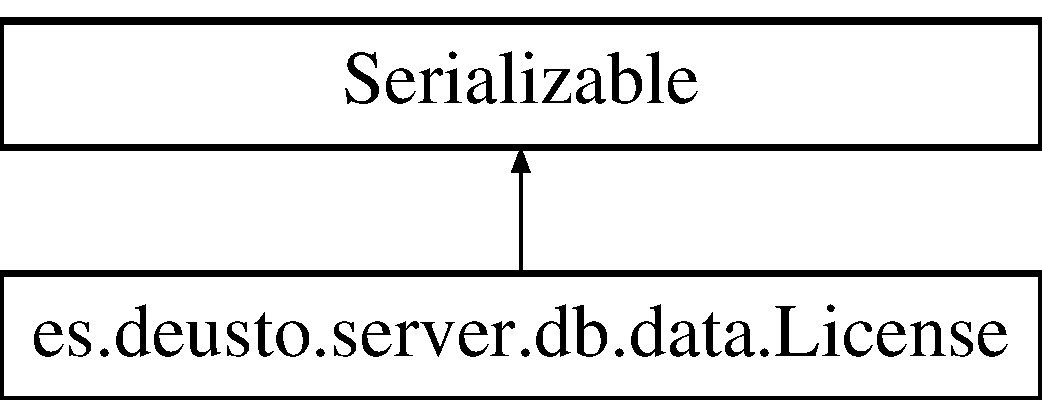
\includegraphics[height=2.000000cm]{classes_1_1deusto_1_1server_1_1db_1_1data_1_1_license}
\end{center}
\end{figure}
\subsection*{Public Member Functions}
\begin{DoxyCompactItemize}
\item 
\hyperlink{classes_1_1deusto_1_1server_1_1db_1_1data_1_1_license_acc02ae536a7b91b4055271fc93ca8957}{License} (String game\+Key)
\item 
boolean \hyperlink{classes_1_1deusto_1_1server_1_1db_1_1data_1_1_license_aac909623c11f10a457f8b7511145036a}{is\+Used} ()
\item 
void \hyperlink{classes_1_1deusto_1_1server_1_1db_1_1data_1_1_license_aa06731eb1852041fbd788167f6ada563}{set\+Used} (boolean is\+Used)
\item 
String \hyperlink{classes_1_1deusto_1_1server_1_1db_1_1data_1_1_license_a2ca537ce43b9036ccff6626fe70205bc}{get\+Game\+Key} ()
\item 
\hyperlink{classes_1_1deusto_1_1server_1_1db_1_1data_1_1_game}{Game} \hyperlink{classes_1_1deusto_1_1server_1_1db_1_1data_1_1_license_a38c4c66098bc5faa947cd6599fc7f90f}{get\+Game} ()
\item 
void \hyperlink{classes_1_1deusto_1_1server_1_1db_1_1data_1_1_license_ab3173591006e39649097242e4a1045cb}{set\+Game} (\hyperlink{classes_1_1deusto_1_1server_1_1db_1_1data_1_1_game}{Game} game)
\item 
\hyperlink{classes_1_1deusto_1_1server_1_1db_1_1data_1_1_user}{User} \hyperlink{classes_1_1deusto_1_1server_1_1db_1_1data_1_1_license_aa7a9c7a2a5c6b4663746ed3e8ccaf0a1}{get\+User} ()
\item 
void \hyperlink{classes_1_1deusto_1_1server_1_1db_1_1data_1_1_license_a3ca25ef2a8e0d28af263d67f3d41e893}{set\+User} (\hyperlink{classes_1_1deusto_1_1server_1_1db_1_1data_1_1_user}{User} user)
\item 
String \hyperlink{classes_1_1deusto_1_1server_1_1db_1_1data_1_1_license_ae8d930f46f5336bb3478d26ef95c578e}{to\+String} ()
\end{DoxyCompactItemize}


\subsection{Detailed Description}


Definition at line 9 of file License.\+java.



\subsection{Constructor \& Destructor Documentation}
\mbox{\Hypertarget{classes_1_1deusto_1_1server_1_1db_1_1data_1_1_license_acc02ae536a7b91b4055271fc93ca8957}\label{classes_1_1deusto_1_1server_1_1db_1_1data_1_1_license_acc02ae536a7b91b4055271fc93ca8957}} 
\index{es\+::deusto\+::server\+::db\+::data\+::\+License@{es\+::deusto\+::server\+::db\+::data\+::\+License}!License@{License}}
\index{License@{License}!es\+::deusto\+::server\+::db\+::data\+::\+License@{es\+::deusto\+::server\+::db\+::data\+::\+License}}
\subsubsection{\texorpdfstring{License()}{License()}}
{\footnotesize\ttfamily es.\+deusto.\+server.\+db.\+data.\+License.\+License (\begin{DoxyParamCaption}\item[{String}]{game\+Key }\end{DoxyParamCaption})}



Definition at line 20 of file License.\+java.



\subsection{Member Function Documentation}
\mbox{\Hypertarget{classes_1_1deusto_1_1server_1_1db_1_1data_1_1_license_a38c4c66098bc5faa947cd6599fc7f90f}\label{classes_1_1deusto_1_1server_1_1db_1_1data_1_1_license_a38c4c66098bc5faa947cd6599fc7f90f}} 
\index{es\+::deusto\+::server\+::db\+::data\+::\+License@{es\+::deusto\+::server\+::db\+::data\+::\+License}!get\+Game@{get\+Game}}
\index{get\+Game@{get\+Game}!es\+::deusto\+::server\+::db\+::data\+::\+License@{es\+::deusto\+::server\+::db\+::data\+::\+License}}
\subsubsection{\texorpdfstring{get\+Game()}{getGame()}}
{\footnotesize\ttfamily \hyperlink{classes_1_1deusto_1_1server_1_1db_1_1data_1_1_game}{Game} es.\+deusto.\+server.\+db.\+data.\+License.\+get\+Game (\begin{DoxyParamCaption}{ }\end{DoxyParamCaption})}



Definition at line 38 of file License.\+java.

\mbox{\Hypertarget{classes_1_1deusto_1_1server_1_1db_1_1data_1_1_license_a2ca537ce43b9036ccff6626fe70205bc}\label{classes_1_1deusto_1_1server_1_1db_1_1data_1_1_license_a2ca537ce43b9036ccff6626fe70205bc}} 
\index{es\+::deusto\+::server\+::db\+::data\+::\+License@{es\+::deusto\+::server\+::db\+::data\+::\+License}!get\+Game\+Key@{get\+Game\+Key}}
\index{get\+Game\+Key@{get\+Game\+Key}!es\+::deusto\+::server\+::db\+::data\+::\+License@{es\+::deusto\+::server\+::db\+::data\+::\+License}}
\subsubsection{\texorpdfstring{get\+Game\+Key()}{getGameKey()}}
{\footnotesize\ttfamily String es.\+deusto.\+server.\+db.\+data.\+License.\+get\+Game\+Key (\begin{DoxyParamCaption}{ }\end{DoxyParamCaption})}



Definition at line 34 of file License.\+java.

\mbox{\Hypertarget{classes_1_1deusto_1_1server_1_1db_1_1data_1_1_license_aa7a9c7a2a5c6b4663746ed3e8ccaf0a1}\label{classes_1_1deusto_1_1server_1_1db_1_1data_1_1_license_aa7a9c7a2a5c6b4663746ed3e8ccaf0a1}} 
\index{es\+::deusto\+::server\+::db\+::data\+::\+License@{es\+::deusto\+::server\+::db\+::data\+::\+License}!get\+User@{get\+User}}
\index{get\+User@{get\+User}!es\+::deusto\+::server\+::db\+::data\+::\+License@{es\+::deusto\+::server\+::db\+::data\+::\+License}}
\subsubsection{\texorpdfstring{get\+User()}{getUser()}}
{\footnotesize\ttfamily \hyperlink{classes_1_1deusto_1_1server_1_1db_1_1data_1_1_user}{User} es.\+deusto.\+server.\+db.\+data.\+License.\+get\+User (\begin{DoxyParamCaption}{ }\end{DoxyParamCaption})}



Definition at line 46 of file License.\+java.

\mbox{\Hypertarget{classes_1_1deusto_1_1server_1_1db_1_1data_1_1_license_aac909623c11f10a457f8b7511145036a}\label{classes_1_1deusto_1_1server_1_1db_1_1data_1_1_license_aac909623c11f10a457f8b7511145036a}} 
\index{es\+::deusto\+::server\+::db\+::data\+::\+License@{es\+::deusto\+::server\+::db\+::data\+::\+License}!is\+Used@{is\+Used}}
\index{is\+Used@{is\+Used}!es\+::deusto\+::server\+::db\+::data\+::\+License@{es\+::deusto\+::server\+::db\+::data\+::\+License}}
\subsubsection{\texorpdfstring{is\+Used()}{isUsed()}}
{\footnotesize\ttfamily boolean es.\+deusto.\+server.\+db.\+data.\+License.\+is\+Used (\begin{DoxyParamCaption}{ }\end{DoxyParamCaption})}



Definition at line 26 of file License.\+java.

\mbox{\Hypertarget{classes_1_1deusto_1_1server_1_1db_1_1data_1_1_license_ab3173591006e39649097242e4a1045cb}\label{classes_1_1deusto_1_1server_1_1db_1_1data_1_1_license_ab3173591006e39649097242e4a1045cb}} 
\index{es\+::deusto\+::server\+::db\+::data\+::\+License@{es\+::deusto\+::server\+::db\+::data\+::\+License}!set\+Game@{set\+Game}}
\index{set\+Game@{set\+Game}!es\+::deusto\+::server\+::db\+::data\+::\+License@{es\+::deusto\+::server\+::db\+::data\+::\+License}}
\subsubsection{\texorpdfstring{set\+Game()}{setGame()}}
{\footnotesize\ttfamily void es.\+deusto.\+server.\+db.\+data.\+License.\+set\+Game (\begin{DoxyParamCaption}\item[{\hyperlink{classes_1_1deusto_1_1server_1_1db_1_1data_1_1_game}{Game}}]{game }\end{DoxyParamCaption})}



Definition at line 42 of file License.\+java.

\mbox{\Hypertarget{classes_1_1deusto_1_1server_1_1db_1_1data_1_1_license_aa06731eb1852041fbd788167f6ada563}\label{classes_1_1deusto_1_1server_1_1db_1_1data_1_1_license_aa06731eb1852041fbd788167f6ada563}} 
\index{es\+::deusto\+::server\+::db\+::data\+::\+License@{es\+::deusto\+::server\+::db\+::data\+::\+License}!set\+Used@{set\+Used}}
\index{set\+Used@{set\+Used}!es\+::deusto\+::server\+::db\+::data\+::\+License@{es\+::deusto\+::server\+::db\+::data\+::\+License}}
\subsubsection{\texorpdfstring{set\+Used()}{setUsed()}}
{\footnotesize\ttfamily void es.\+deusto.\+server.\+db.\+data.\+License.\+set\+Used (\begin{DoxyParamCaption}\item[{boolean}]{is\+Used }\end{DoxyParamCaption})}



Definition at line 30 of file License.\+java.

\mbox{\Hypertarget{classes_1_1deusto_1_1server_1_1db_1_1data_1_1_license_a3ca25ef2a8e0d28af263d67f3d41e893}\label{classes_1_1deusto_1_1server_1_1db_1_1data_1_1_license_a3ca25ef2a8e0d28af263d67f3d41e893}} 
\index{es\+::deusto\+::server\+::db\+::data\+::\+License@{es\+::deusto\+::server\+::db\+::data\+::\+License}!set\+User@{set\+User}}
\index{set\+User@{set\+User}!es\+::deusto\+::server\+::db\+::data\+::\+License@{es\+::deusto\+::server\+::db\+::data\+::\+License}}
\subsubsection{\texorpdfstring{set\+User()}{setUser()}}
{\footnotesize\ttfamily void es.\+deusto.\+server.\+db.\+data.\+License.\+set\+User (\begin{DoxyParamCaption}\item[{\hyperlink{classes_1_1deusto_1_1server_1_1db_1_1data_1_1_user}{User}}]{user }\end{DoxyParamCaption})}



Definition at line 50 of file License.\+java.

\mbox{\Hypertarget{classes_1_1deusto_1_1server_1_1db_1_1data_1_1_license_ae8d930f46f5336bb3478d26ef95c578e}\label{classes_1_1deusto_1_1server_1_1db_1_1data_1_1_license_ae8d930f46f5336bb3478d26ef95c578e}} 
\index{es\+::deusto\+::server\+::db\+::data\+::\+License@{es\+::deusto\+::server\+::db\+::data\+::\+License}!to\+String@{to\+String}}
\index{to\+String@{to\+String}!es\+::deusto\+::server\+::db\+::data\+::\+License@{es\+::deusto\+::server\+::db\+::data\+::\+License}}
\subsubsection{\texorpdfstring{to\+String()}{toString()}}
{\footnotesize\ttfamily String es.\+deusto.\+server.\+db.\+data.\+License.\+to\+String (\begin{DoxyParamCaption}{ }\end{DoxyParamCaption})}



Definition at line 55 of file License.\+java.



The documentation for this class was generated from the following file\+:\begin{DoxyCompactItemize}
\item 
src/main/java/es/deusto/server/db/data/\hyperlink{_license_8java}{License.\+java}\end{DoxyCompactItemize}

\hypertarget{classes_1_1deusto_1_1server_1_1remote_1_1_remote}{}\section{es.\+deusto.\+server.\+remote.\+Remote Class Reference}
\label{classes_1_1deusto_1_1server_1_1remote_1_1_remote}\index{es.\+deusto.\+server.\+remote.\+Remote@{es.\+deusto.\+server.\+remote.\+Remote}}
Inheritance diagram for es.\+deusto.\+server.\+remote.\+Remote\+:\begin{figure}[H]
\begin{center}
\leavevmode
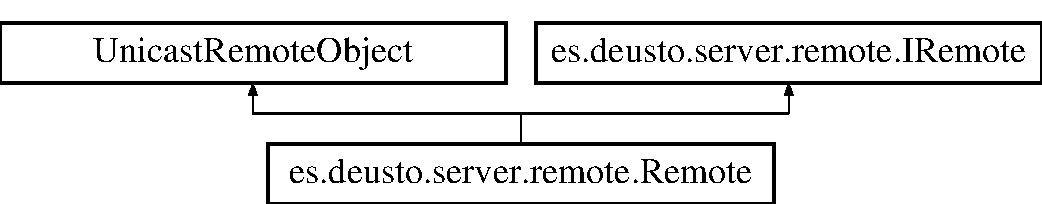
\includegraphics[height=2.000000cm]{classes_1_1deusto_1_1server_1_1remote_1_1_remote}
\end{center}
\end{figure}
\subsection*{Public Member Functions}
\begin{DoxyCompactItemize}
\item 
\hyperlink{classes_1_1deusto_1_1server_1_1remote_1_1_remote_a39055ae30196c2afe97a621b80e43374}{Remote} ()  throws Remote\+Exception 
\item 
boolean \hyperlink{classes_1_1deusto_1_1server_1_1remote_1_1_remote_a1c8e0153dd9b3f6d5499eb6d01e48bbe}{login\+User} (String login, String password)  throws Remote\+Exception 
\item 
boolean \hyperlink{classes_1_1deusto_1_1server_1_1remote_1_1_remote_a4b013f75d23e2c9f0dbca2d3bb467f6a}{register\+User} (String login, String password)  throws Remote\+Exception 
\item 
List$<$ \hyperlink{classes_1_1deusto_1_1server_1_1db_1_1data_1_1_game}{Game} $>$ \hyperlink{classes_1_1deusto_1_1server_1_1remote_1_1_remote_ae40a5882d6b3ef3d5928d87dafeb15fa}{show\+Games\+In\+Store} ()  throws Remote\+Exception 
\item 
void \hyperlink{classes_1_1deusto_1_1server_1_1remote_1_1_remote_aceab50768f98f50ff144b079f229c249}{set\+User\+Wallet} (double k, String login)  throws Remote\+Exception 	
\item 
double \hyperlink{classes_1_1deusto_1_1server_1_1remote_1_1_remote_af7cc190cccf69cda838a6d9805c5c2f5}{get\+User\+Wallet} (String login)  throws Remote\+Exception
\item 
List$<$ \hyperlink{classes_1_1deusto_1_1server_1_1db_1_1data_1_1_game}{Game} $>$ \hyperlink{classes_1_1deusto_1_1server_1_1remote_1_1_remote_a73569877f9317fc48a4e134977baa304}{show\+Owned\+Games} (String username)  throws Remote\+Exception 
\item 
boolean \hyperlink{classes_1_1deusto_1_1server_1_1remote_1_1_remote_ad9f8ad426b1162504b7b39eb1c86d2a3}{buy\+Game} (String username, String name)  throws Remote\+Exception 
\item 
boolean \hyperlink{classes_1_1deusto_1_1server_1_1remote_1_1_remote_ac7d2e76813b61b5a9fcf33d89b6e08c4}{is\+Super\+User} (String login)  throws Remote\+Exception 
\item 
boolean \hyperlink{classes_1_1deusto_1_1server_1_1remote_1_1_remote_a81c61e602f9419408e0069b51bc1e740}{add\+Game} (String g\+Name, double price, double disc, String gg, String c)  throws Remote\+Exception 
\item 
List$<$ String $>$ \hyperlink{classes_1_1deusto_1_1server_1_1remote_1_1_remote_aab476fc9723873e8f85296602d34a97a}{get\+All\+Companies} ()
\item 
List$<$ String $>$ \hyperlink{classes_1_1deusto_1_1server_1_1remote_1_1_remote_a7a276118f167e088bbb56d962b2cc18f}{get\+All\+Genres} ()
\end{DoxyCompactItemize}
\subsection*{Protected Member Functions}
\begin{DoxyCompactItemize}
\item 
void \hyperlink{classes_1_1deusto_1_1server_1_1remote_1_1_remote_ac8c5c24cdafa413da4ad7d71f7f710d3}{finalize} ()  throws Throwable 
\end{DoxyCompactItemize}


\subsection{Detailed Description}
This class checks if the main processes, such as buying a game or registering a user, work correctly \begin{DoxyAuthor}{Author}

\end{DoxyAuthor}
\begin{DoxyVersion}{Version}
1.\+0 
\end{DoxyVersion}
\begin{DoxySince}{Since}
24/03/2017 
\end{DoxySince}


Definition at line 27 of file Remote.\+java.



\subsection{Constructor \& Destructor Documentation}
\mbox{\Hypertarget{classes_1_1deusto_1_1server_1_1remote_1_1_remote_a39055ae30196c2afe97a621b80e43374}\label{classes_1_1deusto_1_1server_1_1remote_1_1_remote_a39055ae30196c2afe97a621b80e43374}} 
\index{es\+::deusto\+::server\+::remote\+::\+Remote@{es\+::deusto\+::server\+::remote\+::\+Remote}!Remote@{Remote}}
\index{Remote@{Remote}!es\+::deusto\+::server\+::remote\+::\+Remote@{es\+::deusto\+::server\+::remote\+::\+Remote}}
\subsubsection{\texorpdfstring{Remote()}{Remote()}}
{\footnotesize\ttfamily es.\+deusto.\+server.\+remote.\+Remote.\+Remote (\begin{DoxyParamCaption}{ }\end{DoxyParamCaption}) throws Remote\+Exception}

This is the constructor for the \hyperlink{classes_1_1deusto_1_1server_1_1remote_1_1_remote}{Remote} class 
\begin{DoxyParams}{Parameters}
{\em unused} & \\
\hline
\end{DoxyParams}
\begin{DoxyReturn}{Returns}
nothing 
\end{DoxyReturn}

\begin{DoxyExceptions}{Exceptions}
{\em Remote\+Exception} & \\
\hline
\end{DoxyExceptions}


Definition at line 41 of file Remote.\+java.



\subsection{Member Function Documentation}
\mbox{\Hypertarget{classes_1_1deusto_1_1server_1_1remote_1_1_remote_a81c61e602f9419408e0069b51bc1e740}\label{classes_1_1deusto_1_1server_1_1remote_1_1_remote_a81c61e602f9419408e0069b51bc1e740}} 
\index{es\+::deusto\+::server\+::remote\+::\+Remote@{es\+::deusto\+::server\+::remote\+::\+Remote}!add\+Game@{add\+Game}}
\index{add\+Game@{add\+Game}!es\+::deusto\+::server\+::remote\+::\+Remote@{es\+::deusto\+::server\+::remote\+::\+Remote}}
\subsubsection{\texorpdfstring{add\+Game()}{addGame()}}
{\footnotesize\ttfamily boolean es.\+deusto.\+server.\+remote.\+Remote.\+add\+Game (\begin{DoxyParamCaption}\item[{String}]{g\+Name,  }\item[{double}]{price,  }\item[{double}]{disc,  }\item[{String}]{gg,  }\item[{String}]{c }\end{DoxyParamCaption}) throws Remote\+Exception}

This method adds a game to the database 
\begin{DoxyParams}{Parameters}
{\em game} & This is the name of a game \\
\hline
{\em genre} & This is the genre of a game \\
\hline
{\em company} & This is the company of a game \\
\hline
\end{DoxyParams}
\begin{DoxyReturn}{Returns}
I\+DB Returns a game stored in the database 
\end{DoxyReturn}

\begin{DoxyExceptions}{Exceptions}
{\em Remote\+Exception} & \\
\hline
\end{DoxyExceptions}
\begin{DoxySeeAlso}{See also}
\hyperlink{interfacees_1_1deusto_1_1server_1_1remote_1_1_i_remote_a991909db4d26d5be67bb3e0bcb501c7e}{es.\+deusto.\+server.\+remote.\+I\+Remote\+::add\+Game}(\hyperlink{classes_1_1deusto_1_1server_1_1db_1_1data_1_1_game}{es.\+deusto.\+server.\+db.\+data.\+Game}, \hyperlink{classes_1_1deusto_1_1server_1_1db_1_1data_1_1_genre}{es.\+deusto.\+server.\+db.\+data.\+Genre}, \hyperlink{classes_1_1deusto_1_1server_1_1db_1_1data_1_1_company}{es.\+deusto.\+server.\+db.\+data.\+Company}) 
\end{DoxySeeAlso}


Implements \hyperlink{interfacees_1_1deusto_1_1server_1_1remote_1_1_i_remote_a991909db4d26d5be67bb3e0bcb501c7e}{es.\+deusto.\+server.\+remote.\+I\+Remote}.



Definition at line 215 of file Remote.\+java.

\mbox{\Hypertarget{classes_1_1deusto_1_1server_1_1remote_1_1_remote_ad9f8ad426b1162504b7b39eb1c86d2a3}\label{classes_1_1deusto_1_1server_1_1remote_1_1_remote_ad9f8ad426b1162504b7b39eb1c86d2a3}} 
\index{es\+::deusto\+::server\+::remote\+::\+Remote@{es\+::deusto\+::server\+::remote\+::\+Remote}!buy\+Game@{buy\+Game}}
\index{buy\+Game@{buy\+Game}!es\+::deusto\+::server\+::remote\+::\+Remote@{es\+::deusto\+::server\+::remote\+::\+Remote}}
\subsubsection{\texorpdfstring{buy\+Game()}{buyGame()}}
{\footnotesize\ttfamily boolean es.\+deusto.\+server.\+remote.\+Remote.\+buy\+Game (\begin{DoxyParamCaption}\item[{String}]{username,  }\item[{String}]{name }\end{DoxyParamCaption}) throws Remote\+Exception}

This method buys a game and adds it to the user owned list 
\begin{DoxyParams}{Parameters}
{\em username} & This is the name of the user \\
\hline
{\em name} & this is the name of a game \\
\hline
\end{DoxyParams}
\begin{DoxyReturn}{Returns}
I\+DB Returns a game stored in the database 
\end{DoxyReturn}

\begin{DoxyExceptions}{Exceptions}
{\em Remote\+Exception} & \\
\hline
\end{DoxyExceptions}
\begin{DoxySeeAlso}{See also}
\hyperlink{interfacees_1_1deusto_1_1server_1_1remote_1_1_i_remote_ad2e6ee616bdc780b4057e63bf2ae8be7}{es.\+deusto.\+server.\+remote.\+I\+Remote\+::buy\+Game}(java.\+lang.\+String, java.\+lang.\+String) 
\end{DoxySeeAlso}


Implements \hyperlink{interfacees_1_1deusto_1_1server_1_1remote_1_1_i_remote_ad2e6ee616bdc780b4057e63bf2ae8be7}{es.\+deusto.\+server.\+remote.\+I\+Remote}.



Definition at line 181 of file Remote.\+java.

\mbox{\Hypertarget{classes_1_1deusto_1_1server_1_1remote_1_1_remote_ac8c5c24cdafa413da4ad7d71f7f710d3}\label{classes_1_1deusto_1_1server_1_1remote_1_1_remote_ac8c5c24cdafa413da4ad7d71f7f710d3}} 
\index{es\+::deusto\+::server\+::remote\+::\+Remote@{es\+::deusto\+::server\+::remote\+::\+Remote}!finalize@{finalize}}
\index{finalize@{finalize}!es\+::deusto\+::server\+::remote\+::\+Remote@{es\+::deusto\+::server\+::remote\+::\+Remote}}
\subsubsection{\texorpdfstring{finalize()}{finalize()}}
{\footnotesize\ttfamily void es.\+deusto.\+server.\+remote.\+Remote.\+finalize (\begin{DoxyParamCaption}{ }\end{DoxyParamCaption}) throws Throwable\hspace{0.3cm}{\ttfamily [protected]}}

This method finalizes the connection with the database 
\begin{DoxyParams}{Parameters}
{\em unused} & \\
\hline
\end{DoxyParams}
\begin{DoxyReturn}{Returns}
none 
\end{DoxyReturn}
\begin{DoxySeeAlso}{See also}
java.\+lang.\+Object\+::finalize() 
\end{DoxySeeAlso}


Definition at line 266 of file Remote.\+java.

\mbox{\Hypertarget{classes_1_1deusto_1_1server_1_1remote_1_1_remote_aab476fc9723873e8f85296602d34a97a}\label{classes_1_1deusto_1_1server_1_1remote_1_1_remote_aab476fc9723873e8f85296602d34a97a}} 
\index{es\+::deusto\+::server\+::remote\+::\+Remote@{es\+::deusto\+::server\+::remote\+::\+Remote}!get\+All\+Companies@{get\+All\+Companies}}
\index{get\+All\+Companies@{get\+All\+Companies}!es\+::deusto\+::server\+::remote\+::\+Remote@{es\+::deusto\+::server\+::remote\+::\+Remote}}
\subsubsection{\texorpdfstring{get\+All\+Companies()}{getAllCompanies()}}
{\footnotesize\ttfamily List$<$String$>$ es.\+deusto.\+server.\+remote.\+Remote.\+get\+All\+Companies (\begin{DoxyParamCaption}{ }\end{DoxyParamCaption})}

This method shows all the companies 
\begin{DoxyParams}{Parameters}
{\em unused} & \\
\hline
\end{DoxyParams}
\begin{DoxyReturn}{Returns}
List$<$\+String$>$ Returns a list of companies 
\end{DoxyReturn}
\begin{DoxySeeAlso}{See also}
\hyperlink{interfacees_1_1deusto_1_1server_1_1remote_1_1_i_remote_a79aad360068d216b63b8afadcc6bcc92}{es.\+deusto.\+server.\+remote.\+I\+Remote\+::get\+All\+Companies()} 
\end{DoxySeeAlso}


Implements \hyperlink{interfacees_1_1deusto_1_1server_1_1remote_1_1_i_remote_a79aad360068d216b63b8afadcc6bcc92}{es.\+deusto.\+server.\+remote.\+I\+Remote}.



Definition at line 229 of file Remote.\+java.

\mbox{\Hypertarget{classes_1_1deusto_1_1server_1_1remote_1_1_remote_a7a276118f167e088bbb56d962b2cc18f}\label{classes_1_1deusto_1_1server_1_1remote_1_1_remote_a7a276118f167e088bbb56d962b2cc18f}} 
\index{es\+::deusto\+::server\+::remote\+::\+Remote@{es\+::deusto\+::server\+::remote\+::\+Remote}!get\+All\+Genres@{get\+All\+Genres}}
\index{get\+All\+Genres@{get\+All\+Genres}!es\+::deusto\+::server\+::remote\+::\+Remote@{es\+::deusto\+::server\+::remote\+::\+Remote}}
\subsubsection{\texorpdfstring{get\+All\+Genres()}{getAllGenres()}}
{\footnotesize\ttfamily List$<$String$>$ es.\+deusto.\+server.\+remote.\+Remote.\+get\+All\+Genres (\begin{DoxyParamCaption}{ }\end{DoxyParamCaption})}

This method shows all the genres 
\begin{DoxyParams}{Parameters}
{\em unused} & \\
\hline
\end{DoxyParams}
\begin{DoxyReturn}{Returns}
List$<$\+String$>$ Returns a list of genres 
\end{DoxyReturn}
\begin{DoxySeeAlso}{See also}
\hyperlink{interfacees_1_1deusto_1_1server_1_1remote_1_1_i_remote_a90995befbd81e0781056f75645997fe9}{es.\+deusto.\+server.\+remote.\+I\+Remote\+::get\+All\+Genres()} 
\end{DoxySeeAlso}


Implements \hyperlink{interfacees_1_1deusto_1_1server_1_1remote_1_1_i_remote_a90995befbd81e0781056f75645997fe9}{es.\+deusto.\+server.\+remote.\+I\+Remote}.



Definition at line 241 of file Remote.\+java.

\mbox{\Hypertarget{classes_1_1deusto_1_1server_1_1remote_1_1_remote_af7cc190cccf69cda838a6d9805c5c2f5}\label{classes_1_1deusto_1_1server_1_1remote_1_1_remote_af7cc190cccf69cda838a6d9805c5c2f5}} 
\index{es\+::deusto\+::server\+::remote\+::\+Remote@{es\+::deusto\+::server\+::remote\+::\+Remote}!get\+User\+Wallet@{get\+User\+Wallet}}
\index{get\+User\+Wallet@{get\+User\+Wallet}!es\+::deusto\+::server\+::remote\+::\+Remote@{es\+::deusto\+::server\+::remote\+::\+Remote}}
\subsubsection{\texorpdfstring{get\+User\+Wallet()}{getUserWallet()}}
{\footnotesize\ttfamily double es.\+deusto.\+server.\+remote.\+Remote.\+get\+User\+Wallet (\begin{DoxyParamCaption}\item[{String}]{login }\end{DoxyParamCaption}) throws Remote\+Exception}

This method shows the wallet of a user 
\begin{DoxyParams}{Parameters}
{\em login} & This is the user login name \\
\hline
\end{DoxyParams}
\begin{DoxyReturn}{Returns}
double Returns the amount of money a user has in the wallet 
\end{DoxyReturn}

\begin{DoxyExceptions}{Exceptions}
{\em Remote\+Exception} & \\
\hline
\end{DoxyExceptions}
\begin{DoxySeeAlso}{See also}
\hyperlink{interfacees_1_1deusto_1_1server_1_1remote_1_1_i_remote_a53305dbc72d910c932e66e2c27c5e1bb}{es.\+deusto.\+server.\+remote.\+I\+Remote\+::get\+User\+Wallet}(java.\+lang.\+String) 
\end{DoxySeeAlso}


Implements \hyperlink{interfacees_1_1deusto_1_1server_1_1remote_1_1_i_remote_a53305dbc72d910c932e66e2c27c5e1bb}{es.\+deusto.\+server.\+remote.\+I\+Remote}.



Definition at line 133 of file Remote.\+java.

\mbox{\Hypertarget{classes_1_1deusto_1_1server_1_1remote_1_1_remote_ac7d2e76813b61b5a9fcf33d89b6e08c4}\label{classes_1_1deusto_1_1server_1_1remote_1_1_remote_ac7d2e76813b61b5a9fcf33d89b6e08c4}} 
\index{es\+::deusto\+::server\+::remote\+::\+Remote@{es\+::deusto\+::server\+::remote\+::\+Remote}!is\+Super\+User@{is\+Super\+User}}
\index{is\+Super\+User@{is\+Super\+User}!es\+::deusto\+::server\+::remote\+::\+Remote@{es\+::deusto\+::server\+::remote\+::\+Remote}}
\subsubsection{\texorpdfstring{is\+Super\+User()}{isSuperUser()}}
{\footnotesize\ttfamily boolean es.\+deusto.\+server.\+remote.\+Remote.\+is\+Super\+User (\begin{DoxyParamCaption}\item[{String}]{login }\end{DoxyParamCaption}) throws Remote\+Exception}

This method shows if a user is superuser or not 
\begin{DoxyParams}{Parameters}
{\em login} & This is the login name of a user \\
\hline
\end{DoxyParams}
\begin{DoxyReturn}{Returns}
boolean Returns if the user is also superuser 
\end{DoxyReturn}
\begin{DoxySeeAlso}{See also}
\hyperlink{interfacees_1_1deusto_1_1server_1_1remote_1_1_i_remote_a488f8b57271876e219af445345428d73}{es.\+deusto.\+server.\+remote.\+I\+Remote\+::is\+Super\+User}(java.\+lang.\+String) 
\end{DoxySeeAlso}


Implements \hyperlink{interfacees_1_1deusto_1_1server_1_1remote_1_1_i_remote_a488f8b57271876e219af445345428d73}{es.\+deusto.\+server.\+remote.\+I\+Remote}.



Definition at line 201 of file Remote.\+java.

\mbox{\Hypertarget{classes_1_1deusto_1_1server_1_1remote_1_1_remote_a1c8e0153dd9b3f6d5499eb6d01e48bbe}\label{classes_1_1deusto_1_1server_1_1remote_1_1_remote_a1c8e0153dd9b3f6d5499eb6d01e48bbe}} 
\index{es\+::deusto\+::server\+::remote\+::\+Remote@{es\+::deusto\+::server\+::remote\+::\+Remote}!login\+User@{login\+User}}
\index{login\+User@{login\+User}!es\+::deusto\+::server\+::remote\+::\+Remote@{es\+::deusto\+::server\+::remote\+::\+Remote}}
\subsubsection{\texorpdfstring{login\+User()}{loginUser()}}
{\footnotesize\ttfamily boolean es.\+deusto.\+server.\+remote.\+Remote.\+login\+User (\begin{DoxyParamCaption}\item[{String}]{login,  }\item[{String}]{password }\end{DoxyParamCaption}) throws Remote\+Exception}

This method allows a user to log in 
\begin{DoxyParams}{Parameters}
{\em login} & This is the login name of a user \\
\hline
{\em password} & This is the login password of a user \\
\hline
\end{DoxyParams}
\begin{DoxyReturn}{Returns}
boolean Returns true if the user can log in and false if not 
\end{DoxyReturn}

\begin{DoxyExceptions}{Exceptions}
{\em Remote\+Exception} & \\
\hline
\end{DoxyExceptions}
\begin{DoxySeeAlso}{See also}
\hyperlink{interfacees_1_1deusto_1_1server_1_1remote_1_1_i_remote_a19acdbd6565b0f00cbe860a3316071ad}{es.\+deusto.\+server.\+remote.\+I\+Remote\+::login\+User}(java.\+lang.\+String, java.\+lang.\+String) 
\end{DoxySeeAlso}


Implements \hyperlink{interfacees_1_1deusto_1_1server_1_1remote_1_1_i_remote_a19acdbd6565b0f00cbe860a3316071ad}{es.\+deusto.\+server.\+remote.\+I\+Remote}.



Definition at line 53 of file Remote.\+java.

\mbox{\Hypertarget{classes_1_1deusto_1_1server_1_1remote_1_1_remote_a4b013f75d23e2c9f0dbca2d3bb467f6a}\label{classes_1_1deusto_1_1server_1_1remote_1_1_remote_a4b013f75d23e2c9f0dbca2d3bb467f6a}} 
\index{es\+::deusto\+::server\+::remote\+::\+Remote@{es\+::deusto\+::server\+::remote\+::\+Remote}!register\+User@{register\+User}}
\index{register\+User@{register\+User}!es\+::deusto\+::server\+::remote\+::\+Remote@{es\+::deusto\+::server\+::remote\+::\+Remote}}
\subsubsection{\texorpdfstring{register\+User()}{registerUser()}}
{\footnotesize\ttfamily boolean es.\+deusto.\+server.\+remote.\+Remote.\+register\+User (\begin{DoxyParamCaption}\item[{String}]{login,  }\item[{String}]{password }\end{DoxyParamCaption}) throws Remote\+Exception}

This method checks if the registration process works correctly 
\begin{DoxyParams}{Parameters}
{\em login} & This is the login name of the user \\
\hline
{\em password} & This is the password for the login \\
\hline
{\em is\+Super\+User} & This is true if the user is a Superuser or false if not \\
\hline
\end{DoxyParams}
\begin{DoxyReturn}{Returns}
I\+DB Returns the registered user in the database 
\end{DoxyReturn}

\begin{DoxyExceptions}{Exceptions}
{\em Remote\+Exception} & \\
\hline
\end{DoxyExceptions}
\begin{DoxySeeAlso}{See also}
\hyperlink{interfacees_1_1deusto_1_1server_1_1remote_1_1_i_remote_aea9a185d69da02d134443a3802a20b32}{es.\+deusto.\+server.\+remote.\+I\+Remote\+::register\+User}(java.\+lang.\+String, java.\+lang.\+String, boolean) 
\end{DoxySeeAlso}


Implements \hyperlink{interfacees_1_1deusto_1_1server_1_1remote_1_1_i_remote_aea9a185d69da02d134443a3802a20b32}{es.\+deusto.\+server.\+remote.\+I\+Remote}.



Definition at line 73 of file Remote.\+java.

\mbox{\Hypertarget{classes_1_1deusto_1_1server_1_1remote_1_1_remote_aceab50768f98f50ff144b079f229c249}\label{classes_1_1deusto_1_1server_1_1remote_1_1_remote_aceab50768f98f50ff144b079f229c249}} 
\index{es\+::deusto\+::server\+::remote\+::\+Remote@{es\+::deusto\+::server\+::remote\+::\+Remote}!set\+User\+Wallet@{set\+User\+Wallet}}
\index{set\+User\+Wallet@{set\+User\+Wallet}!es\+::deusto\+::server\+::remote\+::\+Remote@{es\+::deusto\+::server\+::remote\+::\+Remote}}
\subsubsection{\texorpdfstring{set\+User\+Wallet()}{setUserWallet()}}
{\footnotesize\ttfamily void es.\+deusto.\+server.\+remote.\+Remote.\+set\+User\+Wallet (\begin{DoxyParamCaption}\item[{double}]{k,  }\item[{String}]{login }\end{DoxyParamCaption}) throws Remote\+Exception}

This method changes the amount of money in the wallet 
\begin{DoxyParams}{Parameters}
{\em k} & This is the amount of money \\
\hline
{\em login} & This is the login name of a user \\
\hline
\end{DoxyParams}
\begin{DoxyReturn}{Returns}
nothing 
\end{DoxyReturn}

\begin{DoxyExceptions}{Exceptions}
{\em Remote\+Exception} & \\
\hline
\end{DoxyExceptions}


Implements \hyperlink{interfacees_1_1deusto_1_1server_1_1remote_1_1_i_remote_a6252daae1e76aee233294482f661160a}{es.\+deusto.\+server.\+remote.\+I\+Remote}.



Definition at line 112 of file Remote.\+java.

\mbox{\Hypertarget{classes_1_1deusto_1_1server_1_1remote_1_1_remote_ae40a5882d6b3ef3d5928d87dafeb15fa}\label{classes_1_1deusto_1_1server_1_1remote_1_1_remote_ae40a5882d6b3ef3d5928d87dafeb15fa}} 
\index{es\+::deusto\+::server\+::remote\+::\+Remote@{es\+::deusto\+::server\+::remote\+::\+Remote}!show\+Games\+In\+Store@{show\+Games\+In\+Store}}
\index{show\+Games\+In\+Store@{show\+Games\+In\+Store}!es\+::deusto\+::server\+::remote\+::\+Remote@{es\+::deusto\+::server\+::remote\+::\+Remote}}
\subsubsection{\texorpdfstring{show\+Games\+In\+Store()}{showGamesInStore()}}
{\footnotesize\ttfamily List$<$\hyperlink{classes_1_1deusto_1_1server_1_1db_1_1data_1_1_game}{Game}$>$ es.\+deusto.\+server.\+remote.\+Remote.\+show\+Games\+In\+Store (\begin{DoxyParamCaption}{ }\end{DoxyParamCaption}) throws Remote\+Exception}

This method shows all the games available in the store 
\begin{DoxyParams}{Parameters}
{\em unused} & \\
\hline
\end{DoxyParams}
\begin{DoxyReturn}{Returns}
List Returns a list of games stored in the database 
\end{DoxyReturn}

\begin{DoxyExceptions}{Exceptions}
{\em Remote\+Exception} & \\
\hline
\end{DoxyExceptions}
\begin{DoxySeeAlso}{See also}
\hyperlink{interfacees_1_1deusto_1_1server_1_1remote_1_1_i_remote_a091249da31b567c1be29e07085d3ff18}{es.\+deusto.\+server.\+remote.\+I\+Remote\+::show\+Games\+In\+Store()} 
\end{DoxySeeAlso}


Implements \hyperlink{interfacees_1_1deusto_1_1server_1_1remote_1_1_i_remote_a091249da31b567c1be29e07085d3ff18}{es.\+deusto.\+server.\+remote.\+I\+Remote}.



Definition at line 93 of file Remote.\+java.

\mbox{\Hypertarget{classes_1_1deusto_1_1server_1_1remote_1_1_remote_a73569877f9317fc48a4e134977baa304}\label{classes_1_1deusto_1_1server_1_1remote_1_1_remote_a73569877f9317fc48a4e134977baa304}} 
\index{es\+::deusto\+::server\+::remote\+::\+Remote@{es\+::deusto\+::server\+::remote\+::\+Remote}!show\+Owned\+Games@{show\+Owned\+Games}}
\index{show\+Owned\+Games@{show\+Owned\+Games}!es\+::deusto\+::server\+::remote\+::\+Remote@{es\+::deusto\+::server\+::remote\+::\+Remote}}
\subsubsection{\texorpdfstring{show\+Owned\+Games()}{showOwnedGames()}}
{\footnotesize\ttfamily List$<$\hyperlink{classes_1_1deusto_1_1server_1_1db_1_1data_1_1_game}{Game}$>$ es.\+deusto.\+server.\+remote.\+Remote.\+show\+Owned\+Games (\begin{DoxyParamCaption}\item[{String}]{username }\end{DoxyParamCaption}) throws Remote\+Exception}

This method shows all the games a user owns 
\begin{DoxyParams}{Parameters}
{\em username} & This is the name of the user \\
\hline
\end{DoxyParams}
\begin{DoxyReturn}{Returns}
List Returns a list of games stored in the database 
\end{DoxyReturn}

\begin{DoxyExceptions}{Exceptions}
{\em Remote\+Exception} & \\
\hline
\end{DoxyExceptions}
\begin{DoxySeeAlso}{See also}
\hyperlink{interfacees_1_1deusto_1_1server_1_1remote_1_1_i_remote_aaaf6af5906c81cbd7b3b190a70ead98b}{es.\+deusto.\+server.\+remote.\+I\+Remote\+::show\+Owned\+Games}(java.\+lang.\+String) 
\end{DoxySeeAlso}


Implements \hyperlink{interfacees_1_1deusto_1_1server_1_1remote_1_1_i_remote_aaaf6af5906c81cbd7b3b190a70ead98b}{es.\+deusto.\+server.\+remote.\+I\+Remote}.



Definition at line 156 of file Remote.\+java.



The documentation for this class was generated from the following file\+:\begin{DoxyCompactItemize}
\item 
src/main/java/es/deusto/server/remote/\hyperlink{_remote_8java}{Remote.\+java}\end{DoxyCompactItemize}

\hypertarget{classes_1_1deusto_1_1server_1_1_server}{}\section{es.\+deusto.\+server.\+Server Class Reference}
\label{classes_1_1deusto_1_1server_1_1_server}\index{es.\+deusto.\+server.\+Server@{es.\+deusto.\+server.\+Server}}
\subsection*{Static Public Member Functions}
\begin{DoxyCompactItemize}
\item 
static void \hyperlink{classes_1_1deusto_1_1server_1_1_server_a6a7efaafdac4e7814e4a15046eeeca26}{basic\+Data} ()
\item 
static void \hyperlink{classes_1_1deusto_1_1server_1_1_server_a750bb0d7dbd89246a3602f2e20d03fb5}{main} (String\mbox{[}$\,$\mbox{]} args)
\end{DoxyCompactItemize}


\subsection{Detailed Description}


Definition at line 18 of file Server.\+java.



\subsection{Member Function Documentation}
\mbox{\Hypertarget{classes_1_1deusto_1_1server_1_1_server_a6a7efaafdac4e7814e4a15046eeeca26}\label{classes_1_1deusto_1_1server_1_1_server_a6a7efaafdac4e7814e4a15046eeeca26}} 
\index{es\+::deusto\+::server\+::\+Server@{es\+::deusto\+::server\+::\+Server}!basic\+Data@{basic\+Data}}
\index{basic\+Data@{basic\+Data}!es\+::deusto\+::server\+::\+Server@{es\+::deusto\+::server\+::\+Server}}
\subsubsection{\texorpdfstring{basic\+Data()}{basicData()}}
{\footnotesize\ttfamily static void es.\+deusto.\+server.\+Server.\+basic\+Data (\begin{DoxyParamCaption}{ }\end{DoxyParamCaption})\hspace{0.3cm}{\ttfamily [static]}}



Definition at line 21 of file Server.\+java.

\mbox{\Hypertarget{classes_1_1deusto_1_1server_1_1_server_a750bb0d7dbd89246a3602f2e20d03fb5}\label{classes_1_1deusto_1_1server_1_1_server_a750bb0d7dbd89246a3602f2e20d03fb5}} 
\index{es\+::deusto\+::server\+::\+Server@{es\+::deusto\+::server\+::\+Server}!main@{main}}
\index{main@{main}!es\+::deusto\+::server\+::\+Server@{es\+::deusto\+::server\+::\+Server}}
\subsubsection{\texorpdfstring{main()}{main()}}
{\footnotesize\ttfamily static void es.\+deusto.\+server.\+Server.\+main (\begin{DoxyParamCaption}\item[{String \mbox{[}$\,$\mbox{]}}]{args }\end{DoxyParamCaption})\hspace{0.3cm}{\ttfamily [static]}}



Definition at line 55 of file Server.\+java.



The documentation for this class was generated from the following file\+:\begin{DoxyCompactItemize}
\item 
C\+:/\+Users/\+Marta/\+S\+P\+Q09/\+Lurrun/src/main/java/es/deusto/server/\hyperlink{_server_8java}{Server.\+java}\end{DoxyCompactItemize}

\hypertarget{classes_1_1deusto_1_1server_1_1db_1_1data_1_1_user}{}\section{es.\+deusto.\+server.\+db.\+data.\+User Class Reference}
\label{classes_1_1deusto_1_1server_1_1db_1_1data_1_1_user}\index{es.\+deusto.\+server.\+db.\+data.\+User@{es.\+deusto.\+server.\+db.\+data.\+User}}
Inheritance diagram for es.\+deusto.\+server.\+db.\+data.\+User\+:\begin{figure}[H]
\begin{center}
\leavevmode
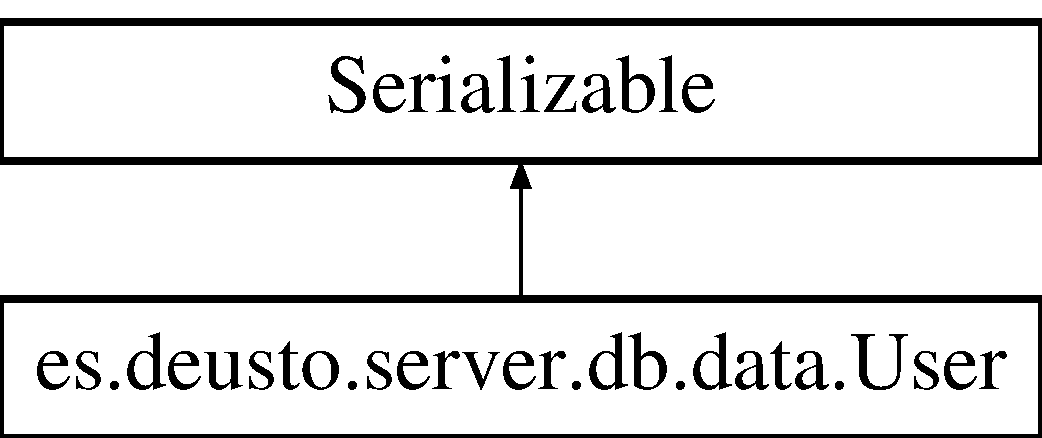
\includegraphics[height=2.000000cm]{classes_1_1deusto_1_1server_1_1db_1_1data_1_1_user}
\end{center}
\end{figure}
\subsection*{Public Member Functions}
\begin{DoxyCompactItemize}
\item 
\hyperlink{classes_1_1deusto_1_1server_1_1db_1_1data_1_1_user_a99b61ff1f905036e1aeea2813a2fb1c1}{User} (String login, String password, boolean is\+Superuser)
\item 
\hyperlink{classes_1_1deusto_1_1server_1_1db_1_1data_1_1_user_accf4cd75adc5bfc6cd376a1714517ba9}{User} (String login, String password)
\item 
boolean \hyperlink{classes_1_1deusto_1_1server_1_1db_1_1data_1_1_user_a3b6d6d064ccfe7e0dc2a7c6c132cdfc0}{get\+Superuser} ()
\item 
void \hyperlink{classes_1_1deusto_1_1server_1_1db_1_1data_1_1_user_a386c51067e68570828d9dcd130e6fe74}{set\+Superuser} (boolean is\+Superuser)
\item 
void \hyperlink{classes_1_1deusto_1_1server_1_1db_1_1data_1_1_user_a1eefc1e49d4bf8046f3a7cdbca7f670d}{add\+License} (\hyperlink{classes_1_1deusto_1_1server_1_1db_1_1data_1_1_license}{License} license)
\item 
void \hyperlink{classes_1_1deusto_1_1server_1_1db_1_1data_1_1_user_a5ee17c4a3ab4eceb028a087f96527375}{remove\+License} (\hyperlink{classes_1_1deusto_1_1server_1_1db_1_1data_1_1_license}{License} license)
\item 
List$<$ \hyperlink{classes_1_1deusto_1_1server_1_1db_1_1data_1_1_license}{License} $>$ \hyperlink{classes_1_1deusto_1_1server_1_1db_1_1data_1_1_user_adeddbb54df77d3779f739f27959588e1}{get\+Licenses} ()
\item 
String \hyperlink{classes_1_1deusto_1_1server_1_1db_1_1data_1_1_user_a2bc07e76806b027ef70b5ad8cea5f9fa}{get\+Login} ()
\item 
String \hyperlink{classes_1_1deusto_1_1server_1_1db_1_1data_1_1_user_ac576607b3eae9e9b8c7002d5cd7c1a62}{get\+Password} ()
\item 
double \hyperlink{classes_1_1deusto_1_1server_1_1db_1_1data_1_1_user_a28bcff322718c86a4c69dcff039ecf16}{get\+Money} ()
\item 
void \hyperlink{classes_1_1deusto_1_1server_1_1db_1_1data_1_1_user_af7fe255820b6ddd9020c24994cdc6e23}{set\+Money} (double money)
\item 
boolean \hyperlink{classes_1_1deusto_1_1server_1_1db_1_1data_1_1_user_a9dee5f17849d7718c225034d384844ae}{compare\+User\+To} (\hyperlink{classes_1_1deusto_1_1server_1_1db_1_1data_1_1_user}{User} u2)
\item 
String \hyperlink{classes_1_1deusto_1_1server_1_1db_1_1data_1_1_user_a494980951c4c71c0a793994b7bcd5101}{to\+String} ()
\end{DoxyCompactItemize}


\subsection{Detailed Description}


Definition at line 13 of file User.\+java.



\subsection{Constructor \& Destructor Documentation}
\mbox{\Hypertarget{classes_1_1deusto_1_1server_1_1db_1_1data_1_1_user_a99b61ff1f905036e1aeea2813a2fb1c1}\label{classes_1_1deusto_1_1server_1_1db_1_1data_1_1_user_a99b61ff1f905036e1aeea2813a2fb1c1}} 
\index{es\+::deusto\+::server\+::db\+::data\+::\+User@{es\+::deusto\+::server\+::db\+::data\+::\+User}!User@{User}}
\index{User@{User}!es\+::deusto\+::server\+::db\+::data\+::\+User@{es\+::deusto\+::server\+::db\+::data\+::\+User}}
\subsubsection{\texorpdfstring{User()}{User()}\hspace{0.1cm}{\footnotesize\ttfamily [1/2]}}
{\footnotesize\ttfamily es.\+deusto.\+server.\+db.\+data.\+User.\+User (\begin{DoxyParamCaption}\item[{String}]{login,  }\item[{String}]{password,  }\item[{boolean}]{is\+Superuser }\end{DoxyParamCaption})}



Definition at line 25 of file User.\+java.

\mbox{\Hypertarget{classes_1_1deusto_1_1server_1_1db_1_1data_1_1_user_accf4cd75adc5bfc6cd376a1714517ba9}\label{classes_1_1deusto_1_1server_1_1db_1_1data_1_1_user_accf4cd75adc5bfc6cd376a1714517ba9}} 
\index{es\+::deusto\+::server\+::db\+::data\+::\+User@{es\+::deusto\+::server\+::db\+::data\+::\+User}!User@{User}}
\index{User@{User}!es\+::deusto\+::server\+::db\+::data\+::\+User@{es\+::deusto\+::server\+::db\+::data\+::\+User}}
\subsubsection{\texorpdfstring{User()}{User()}\hspace{0.1cm}{\footnotesize\ttfamily [2/2]}}
{\footnotesize\ttfamily es.\+deusto.\+server.\+db.\+data.\+User.\+User (\begin{DoxyParamCaption}\item[{String}]{login,  }\item[{String}]{password }\end{DoxyParamCaption})}



Definition at line 33 of file User.\+java.



\subsection{Member Function Documentation}
\mbox{\Hypertarget{classes_1_1deusto_1_1server_1_1db_1_1data_1_1_user_a1eefc1e49d4bf8046f3a7cdbca7f670d}\label{classes_1_1deusto_1_1server_1_1db_1_1data_1_1_user_a1eefc1e49d4bf8046f3a7cdbca7f670d}} 
\index{es\+::deusto\+::server\+::db\+::data\+::\+User@{es\+::deusto\+::server\+::db\+::data\+::\+User}!add\+License@{add\+License}}
\index{add\+License@{add\+License}!es\+::deusto\+::server\+::db\+::data\+::\+User@{es\+::deusto\+::server\+::db\+::data\+::\+User}}
\subsubsection{\texorpdfstring{add\+License()}{addLicense()}}
{\footnotesize\ttfamily void es.\+deusto.\+server.\+db.\+data.\+User.\+add\+License (\begin{DoxyParamCaption}\item[{\hyperlink{classes_1_1deusto_1_1server_1_1db_1_1data_1_1_license}{License}}]{license }\end{DoxyParamCaption})}



Definition at line 47 of file User.\+java.

\mbox{\Hypertarget{classes_1_1deusto_1_1server_1_1db_1_1data_1_1_user_a9dee5f17849d7718c225034d384844ae}\label{classes_1_1deusto_1_1server_1_1db_1_1data_1_1_user_a9dee5f17849d7718c225034d384844ae}} 
\index{es\+::deusto\+::server\+::db\+::data\+::\+User@{es\+::deusto\+::server\+::db\+::data\+::\+User}!compare\+User\+To@{compare\+User\+To}}
\index{compare\+User\+To@{compare\+User\+To}!es\+::deusto\+::server\+::db\+::data\+::\+User@{es\+::deusto\+::server\+::db\+::data\+::\+User}}
\subsubsection{\texorpdfstring{compare\+User\+To()}{compareUserTo()}}
{\footnotesize\ttfamily boolean es.\+deusto.\+server.\+db.\+data.\+User.\+compare\+User\+To (\begin{DoxyParamCaption}\item[{\hyperlink{classes_1_1deusto_1_1server_1_1db_1_1data_1_1_user}{User}}]{u2 }\end{DoxyParamCaption})}



Definition at line 76 of file User.\+java.

\mbox{\Hypertarget{classes_1_1deusto_1_1server_1_1db_1_1data_1_1_user_adeddbb54df77d3779f739f27959588e1}\label{classes_1_1deusto_1_1server_1_1db_1_1data_1_1_user_adeddbb54df77d3779f739f27959588e1}} 
\index{es\+::deusto\+::server\+::db\+::data\+::\+User@{es\+::deusto\+::server\+::db\+::data\+::\+User}!get\+Licenses@{get\+Licenses}}
\index{get\+Licenses@{get\+Licenses}!es\+::deusto\+::server\+::db\+::data\+::\+User@{es\+::deusto\+::server\+::db\+::data\+::\+User}}
\subsubsection{\texorpdfstring{get\+Licenses()}{getLicenses()}}
{\footnotesize\ttfamily List$<$\hyperlink{classes_1_1deusto_1_1server_1_1db_1_1data_1_1_license}{License}$>$ es.\+deusto.\+server.\+db.\+data.\+User.\+get\+Licenses (\begin{DoxyParamCaption}{ }\end{DoxyParamCaption})}



Definition at line 55 of file User.\+java.

\mbox{\Hypertarget{classes_1_1deusto_1_1server_1_1db_1_1data_1_1_user_a2bc07e76806b027ef70b5ad8cea5f9fa}\label{classes_1_1deusto_1_1server_1_1db_1_1data_1_1_user_a2bc07e76806b027ef70b5ad8cea5f9fa}} 
\index{es\+::deusto\+::server\+::db\+::data\+::\+User@{es\+::deusto\+::server\+::db\+::data\+::\+User}!get\+Login@{get\+Login}}
\index{get\+Login@{get\+Login}!es\+::deusto\+::server\+::db\+::data\+::\+User@{es\+::deusto\+::server\+::db\+::data\+::\+User}}
\subsubsection{\texorpdfstring{get\+Login()}{getLogin()}}
{\footnotesize\ttfamily String es.\+deusto.\+server.\+db.\+data.\+User.\+get\+Login (\begin{DoxyParamCaption}{ }\end{DoxyParamCaption})}



Definition at line 60 of file User.\+java.

\mbox{\Hypertarget{classes_1_1deusto_1_1server_1_1db_1_1data_1_1_user_a28bcff322718c86a4c69dcff039ecf16}\label{classes_1_1deusto_1_1server_1_1db_1_1data_1_1_user_a28bcff322718c86a4c69dcff039ecf16}} 
\index{es\+::deusto\+::server\+::db\+::data\+::\+User@{es\+::deusto\+::server\+::db\+::data\+::\+User}!get\+Money@{get\+Money}}
\index{get\+Money@{get\+Money}!es\+::deusto\+::server\+::db\+::data\+::\+User@{es\+::deusto\+::server\+::db\+::data\+::\+User}}
\subsubsection{\texorpdfstring{get\+Money()}{getMoney()}}
{\footnotesize\ttfamily double es.\+deusto.\+server.\+db.\+data.\+User.\+get\+Money (\begin{DoxyParamCaption}{ }\end{DoxyParamCaption})}



Definition at line 68 of file User.\+java.

\mbox{\Hypertarget{classes_1_1deusto_1_1server_1_1db_1_1data_1_1_user_ac576607b3eae9e9b8c7002d5cd7c1a62}\label{classes_1_1deusto_1_1server_1_1db_1_1data_1_1_user_ac576607b3eae9e9b8c7002d5cd7c1a62}} 
\index{es\+::deusto\+::server\+::db\+::data\+::\+User@{es\+::deusto\+::server\+::db\+::data\+::\+User}!get\+Password@{get\+Password}}
\index{get\+Password@{get\+Password}!es\+::deusto\+::server\+::db\+::data\+::\+User@{es\+::deusto\+::server\+::db\+::data\+::\+User}}
\subsubsection{\texorpdfstring{get\+Password()}{getPassword()}}
{\footnotesize\ttfamily String es.\+deusto.\+server.\+db.\+data.\+User.\+get\+Password (\begin{DoxyParamCaption}{ }\end{DoxyParamCaption})}



Definition at line 64 of file User.\+java.

\mbox{\Hypertarget{classes_1_1deusto_1_1server_1_1db_1_1data_1_1_user_a3b6d6d064ccfe7e0dc2a7c6c132cdfc0}\label{classes_1_1deusto_1_1server_1_1db_1_1data_1_1_user_a3b6d6d064ccfe7e0dc2a7c6c132cdfc0}} 
\index{es\+::deusto\+::server\+::db\+::data\+::\+User@{es\+::deusto\+::server\+::db\+::data\+::\+User}!get\+Superuser@{get\+Superuser}}
\index{get\+Superuser@{get\+Superuser}!es\+::deusto\+::server\+::db\+::data\+::\+User@{es\+::deusto\+::server\+::db\+::data\+::\+User}}
\subsubsection{\texorpdfstring{get\+Superuser()}{getSuperuser()}}
{\footnotesize\ttfamily boolean es.\+deusto.\+server.\+db.\+data.\+User.\+get\+Superuser (\begin{DoxyParamCaption}{ }\end{DoxyParamCaption})}



Definition at line 39 of file User.\+java.

\mbox{\Hypertarget{classes_1_1deusto_1_1server_1_1db_1_1data_1_1_user_a5ee17c4a3ab4eceb028a087f96527375}\label{classes_1_1deusto_1_1server_1_1db_1_1data_1_1_user_a5ee17c4a3ab4eceb028a087f96527375}} 
\index{es\+::deusto\+::server\+::db\+::data\+::\+User@{es\+::deusto\+::server\+::db\+::data\+::\+User}!remove\+License@{remove\+License}}
\index{remove\+License@{remove\+License}!es\+::deusto\+::server\+::db\+::data\+::\+User@{es\+::deusto\+::server\+::db\+::data\+::\+User}}
\subsubsection{\texorpdfstring{remove\+License()}{removeLicense()}}
{\footnotesize\ttfamily void es.\+deusto.\+server.\+db.\+data.\+User.\+remove\+License (\begin{DoxyParamCaption}\item[{\hyperlink{classes_1_1deusto_1_1server_1_1db_1_1data_1_1_license}{License}}]{license }\end{DoxyParamCaption})}



Definition at line 51 of file User.\+java.

\mbox{\Hypertarget{classes_1_1deusto_1_1server_1_1db_1_1data_1_1_user_af7fe255820b6ddd9020c24994cdc6e23}\label{classes_1_1deusto_1_1server_1_1db_1_1data_1_1_user_af7fe255820b6ddd9020c24994cdc6e23}} 
\index{es\+::deusto\+::server\+::db\+::data\+::\+User@{es\+::deusto\+::server\+::db\+::data\+::\+User}!set\+Money@{set\+Money}}
\index{set\+Money@{set\+Money}!es\+::deusto\+::server\+::db\+::data\+::\+User@{es\+::deusto\+::server\+::db\+::data\+::\+User}}
\subsubsection{\texorpdfstring{set\+Money()}{setMoney()}}
{\footnotesize\ttfamily void es.\+deusto.\+server.\+db.\+data.\+User.\+set\+Money (\begin{DoxyParamCaption}\item[{double}]{money }\end{DoxyParamCaption})}



Definition at line 72 of file User.\+java.

\mbox{\Hypertarget{classes_1_1deusto_1_1server_1_1db_1_1data_1_1_user_a386c51067e68570828d9dcd130e6fe74}\label{classes_1_1deusto_1_1server_1_1db_1_1data_1_1_user_a386c51067e68570828d9dcd130e6fe74}} 
\index{es\+::deusto\+::server\+::db\+::data\+::\+User@{es\+::deusto\+::server\+::db\+::data\+::\+User}!set\+Superuser@{set\+Superuser}}
\index{set\+Superuser@{set\+Superuser}!es\+::deusto\+::server\+::db\+::data\+::\+User@{es\+::deusto\+::server\+::db\+::data\+::\+User}}
\subsubsection{\texorpdfstring{set\+Superuser()}{setSuperuser()}}
{\footnotesize\ttfamily void es.\+deusto.\+server.\+db.\+data.\+User.\+set\+Superuser (\begin{DoxyParamCaption}\item[{boolean}]{is\+Superuser }\end{DoxyParamCaption})}



Definition at line 43 of file User.\+java.

\mbox{\Hypertarget{classes_1_1deusto_1_1server_1_1db_1_1data_1_1_user_a494980951c4c71c0a793994b7bcd5101}\label{classes_1_1deusto_1_1server_1_1db_1_1data_1_1_user_a494980951c4c71c0a793994b7bcd5101}} 
\index{es\+::deusto\+::server\+::db\+::data\+::\+User@{es\+::deusto\+::server\+::db\+::data\+::\+User}!to\+String@{to\+String}}
\index{to\+String@{to\+String}!es\+::deusto\+::server\+::db\+::data\+::\+User@{es\+::deusto\+::server\+::db\+::data\+::\+User}}
\subsubsection{\texorpdfstring{to\+String()}{toString()}}
{\footnotesize\ttfamily String es.\+deusto.\+server.\+db.\+data.\+User.\+to\+String (\begin{DoxyParamCaption}{ }\end{DoxyParamCaption})}



Definition at line 85 of file User.\+java.



The documentation for this class was generated from the following file\+:\begin{DoxyCompactItemize}
\item 
src/main/java/es/deusto/server/db/data/\hyperlink{_user_8java}{User.\+java}\end{DoxyCompactItemize}

\chapter{File Documentation}
\hypertarget{_client_8java}{}\section{C\+:/\+Users/\+Marta/\+S\+P\+Q09/\+Lurrun/src/main/java/es/deusto/client/\+Client.java File Reference}
\label{_client_8java}\index{C\+:/\+Users/\+Marta/\+S\+P\+Q09/\+Lurrun/src/main/java/es/deusto/client/\+Client.\+java@{C\+:/\+Users/\+Marta/\+S\+P\+Q09/\+Lurrun/src/main/java/es/deusto/client/\+Client.\+java}}
\subsection*{Classes}
\begin{DoxyCompactItemize}
\item 
class \hyperlink{classes_1_1deusto_1_1client_1_1_client}{es.\+deusto.\+client.\+Client}
\end{DoxyCompactItemize}
\subsection*{Packages}
\begin{DoxyCompactItemize}
\item 
package \hyperlink{namespacees_1_1deusto_1_1client}{es.\+deusto.\+client}
\end{DoxyCompactItemize}

\hypertarget{_g_u_i_8java}{}\section{src/main/java/es/deusto/client/\+G\+UI.java File Reference}
\label{_g_u_i_8java}\index{src/main/java/es/deusto/client/\+G\+U\+I.\+java@{src/main/java/es/deusto/client/\+G\+U\+I.\+java}}
\subsection*{Classes}
\begin{DoxyCompactItemize}
\item 
class \hyperlink{classes_1_1deusto_1_1client_1_1_g_u_i}{es.\+deusto.\+client.\+G\+UI}
\end{DoxyCompactItemize}
\subsection*{Packages}
\begin{DoxyCompactItemize}
\item 
package \hyperlink{namespacees_1_1deusto_1_1client}{es.\+deusto.\+client}
\end{DoxyCompactItemize}

\hypertarget{_d_a_o_8java}{}\section{C\+:/\+Users/\+Marta/\+S\+P\+Q09/\+Lurrun/src/main/java/es/deusto/server/db/dao/\+D\+AO.java File Reference}
\label{_d_a_o_8java}\index{C\+:/\+Users/\+Marta/\+S\+P\+Q09/\+Lurrun/src/main/java/es/deusto/server/db/dao/\+D\+A\+O.\+java@{C\+:/\+Users/\+Marta/\+S\+P\+Q09/\+Lurrun/src/main/java/es/deusto/server/db/dao/\+D\+A\+O.\+java}}
\subsection*{Classes}
\begin{DoxyCompactItemize}
\item 
class \hyperlink{classes_1_1deusto_1_1server_1_1db_1_1dao_1_1_d_a_o}{es.\+deusto.\+server.\+db.\+dao.\+D\+AO}
\end{DoxyCompactItemize}
\subsection*{Packages}
\begin{DoxyCompactItemize}
\item 
package \hyperlink{namespacees_1_1deusto_1_1server_1_1db_1_1dao}{es.\+deusto.\+server.\+db.\+dao}
\end{DoxyCompactItemize}

\hypertarget{_i_d_a_o_8java}{}\section{src/main/java/es/deusto/server/db/dao/\+I\+D\+AO.java File Reference}
\label{_i_d_a_o_8java}\index{src/main/java/es/deusto/server/db/dao/\+I\+D\+A\+O.\+java@{src/main/java/es/deusto/server/db/dao/\+I\+D\+A\+O.\+java}}
\subsection*{Classes}
\begin{DoxyCompactItemize}
\item 
interface \hyperlink{interfacees_1_1deusto_1_1server_1_1db_1_1dao_1_1_i_d_a_o}{es.\+deusto.\+server.\+db.\+dao.\+I\+D\+AO}
\end{DoxyCompactItemize}
\subsection*{Packages}
\begin{DoxyCompactItemize}
\item 
package \hyperlink{namespacees_1_1deusto_1_1server_1_1db_1_1dao}{es.\+deusto.\+server.\+db.\+dao}
\end{DoxyCompactItemize}

\hypertarget{_company_8java}{}\section{src/main/java/es/deusto/server/db/data/\+Company.java File Reference}
\label{_company_8java}\index{src/main/java/es/deusto/server/db/data/\+Company.\+java@{src/main/java/es/deusto/server/db/data/\+Company.\+java}}
\subsection*{Classes}
\begin{DoxyCompactItemize}
\item 
class \hyperlink{classes_1_1deusto_1_1server_1_1db_1_1data_1_1_company}{es.\+deusto.\+server.\+db.\+data.\+Company}
\end{DoxyCompactItemize}
\subsection*{Packages}
\begin{DoxyCompactItemize}
\item 
package \hyperlink{namespacees_1_1deusto_1_1server_1_1db_1_1data}{es.\+deusto.\+server.\+db.\+data}
\end{DoxyCompactItemize}

\hypertarget{_game_8java}{}\section{C\+:/\+Users/\+Carazo\+\_\+laptop/git/\+S\+P\+Q09/\+Lurrun/src/main/java/es/deusto/server/db/data/\+Game.java File Reference}
\label{_game_8java}\index{C\+:/\+Users/\+Carazo\+\_\+laptop/git/\+S\+P\+Q09/\+Lurrun/src/main/java/es/deusto/server/db/data/\+Game.\+java@{C\+:/\+Users/\+Carazo\+\_\+laptop/git/\+S\+P\+Q09/\+Lurrun/src/main/java/es/deusto/server/db/data/\+Game.\+java}}
\subsection*{Classes}
\begin{DoxyCompactItemize}
\item 
class \hyperlink{classes_1_1deusto_1_1server_1_1db_1_1data_1_1_game}{es.\+deusto.\+server.\+db.\+data.\+Game}
\end{DoxyCompactItemize}
\subsection*{Packages}
\begin{DoxyCompactItemize}
\item 
package \hyperlink{namespacees_1_1deusto_1_1server_1_1db_1_1data}{es.\+deusto.\+server.\+db.\+data}
\end{DoxyCompactItemize}

\hypertarget{_genre_8java}{}\section{C\+:/\+Users/\+Marta/\+S\+P\+Q09/\+Lurrun/src/main/java/es/deusto/server/db/data/\+Genre.java File Reference}
\label{_genre_8java}\index{C\+:/\+Users/\+Marta/\+S\+P\+Q09/\+Lurrun/src/main/java/es/deusto/server/db/data/\+Genre.\+java@{C\+:/\+Users/\+Marta/\+S\+P\+Q09/\+Lurrun/src/main/java/es/deusto/server/db/data/\+Genre.\+java}}
\subsection*{Classes}
\begin{DoxyCompactItemize}
\item 
class \hyperlink{classes_1_1deusto_1_1server_1_1db_1_1data_1_1_genre}{es.\+deusto.\+server.\+db.\+data.\+Genre}
\end{DoxyCompactItemize}
\subsection*{Packages}
\begin{DoxyCompactItemize}
\item 
package \hyperlink{namespacees_1_1deusto_1_1server_1_1db_1_1data}{es.\+deusto.\+server.\+db.\+data}
\end{DoxyCompactItemize}

\hypertarget{_license_8java}{}\section{C\+:/\+Users/\+Marta/\+S\+P\+Q09/\+Lurrun/src/main/java/es/deusto/server/db/data/\+License.java File Reference}
\label{_license_8java}\index{C\+:/\+Users/\+Marta/\+S\+P\+Q09/\+Lurrun/src/main/java/es/deusto/server/db/data/\+License.\+java@{C\+:/\+Users/\+Marta/\+S\+P\+Q09/\+Lurrun/src/main/java/es/deusto/server/db/data/\+License.\+java}}
\subsection*{Classes}
\begin{DoxyCompactItemize}
\item 
class \hyperlink{classes_1_1deusto_1_1server_1_1db_1_1data_1_1_license}{es.\+deusto.\+server.\+db.\+data.\+License}
\end{DoxyCompactItemize}
\subsection*{Packages}
\begin{DoxyCompactItemize}
\item 
package \hyperlink{namespacees_1_1deusto_1_1server_1_1db_1_1data}{es.\+deusto.\+server.\+db.\+data}
\end{DoxyCompactItemize}

\hypertarget{_user_8java}{}\section{C\+:/\+Users/\+Carazo\+\_\+laptop/git/\+S\+P\+Q09/\+Lurrun/src/main/java/es/deusto/server/db/data/\+User.java File Reference}
\label{_user_8java}\index{C\+:/\+Users/\+Carazo\+\_\+laptop/git/\+S\+P\+Q09/\+Lurrun/src/main/java/es/deusto/server/db/data/\+User.\+java@{C\+:/\+Users/\+Carazo\+\_\+laptop/git/\+S\+P\+Q09/\+Lurrun/src/main/java/es/deusto/server/db/data/\+User.\+java}}
\subsection*{Classes}
\begin{DoxyCompactItemize}
\item 
class \hyperlink{classes_1_1deusto_1_1server_1_1db_1_1data_1_1_user}{es.\+deusto.\+server.\+db.\+data.\+User}
\end{DoxyCompactItemize}
\subsection*{Packages}
\begin{DoxyCompactItemize}
\item 
package \hyperlink{namespacees_1_1deusto_1_1server_1_1db_1_1data}{es.\+deusto.\+server.\+db.\+data}
\end{DoxyCompactItemize}

\hypertarget{_d_b_8java}{}\section{C\+:/\+Users/\+Marta/\+S\+P\+Q09/\+Lurrun/src/main/java/es/deusto/server/db/\+DB.java File Reference}
\label{_d_b_8java}\index{C\+:/\+Users/\+Marta/\+S\+P\+Q09/\+Lurrun/src/main/java/es/deusto/server/db/\+D\+B.\+java@{C\+:/\+Users/\+Marta/\+S\+P\+Q09/\+Lurrun/src/main/java/es/deusto/server/db/\+D\+B.\+java}}
\subsection*{Classes}
\begin{DoxyCompactItemize}
\item 
class \hyperlink{classes_1_1deusto_1_1server_1_1db_1_1_d_b}{es.\+deusto.\+server.\+db.\+DB}
\end{DoxyCompactItemize}
\subsection*{Packages}
\begin{DoxyCompactItemize}
\item 
package \hyperlink{namespacees_1_1deusto_1_1server_1_1db}{es.\+deusto.\+server.\+db}
\end{DoxyCompactItemize}

\hypertarget{_i_d_b_8java}{}\section{src/main/java/es/deusto/server/db/\+I\+DB.java File Reference}
\label{_i_d_b_8java}\index{src/main/java/es/deusto/server/db/\+I\+D\+B.\+java@{src/main/java/es/deusto/server/db/\+I\+D\+B.\+java}}
\subsection*{Classes}
\begin{DoxyCompactItemize}
\item 
interface \hyperlink{interfacees_1_1deusto_1_1server_1_1db_1_1_i_d_b}{es.\+deusto.\+server.\+db.\+I\+DB}
\end{DoxyCompactItemize}
\subsection*{Packages}
\begin{DoxyCompactItemize}
\item 
package \hyperlink{namespacees_1_1deusto_1_1server_1_1db}{es.\+deusto.\+server.\+db}
\end{DoxyCompactItemize}

\hypertarget{_i_remote_8java}{}\section{C\+:/\+Users/\+Marta/\+S\+P\+Q09/\+Lurrun/src/main/java/es/deusto/server/remote/\+I\+Remote.java File Reference}
\label{_i_remote_8java}\index{C\+:/\+Users/\+Marta/\+S\+P\+Q09/\+Lurrun/src/main/java/es/deusto/server/remote/\+I\+Remote.\+java@{C\+:/\+Users/\+Marta/\+S\+P\+Q09/\+Lurrun/src/main/java/es/deusto/server/remote/\+I\+Remote.\+java}}
\subsection*{Classes}
\begin{DoxyCompactItemize}
\item 
interface \hyperlink{interfacees_1_1deusto_1_1server_1_1remote_1_1_i_remote}{es.\+deusto.\+server.\+remote.\+I\+Remote}
\end{DoxyCompactItemize}
\subsection*{Packages}
\begin{DoxyCompactItemize}
\item 
package \hyperlink{namespacees_1_1deusto_1_1server_1_1remote}{es.\+deusto.\+server.\+remote}
\end{DoxyCompactItemize}

\hypertarget{_remote_8java}{}\section{src/main/java/es/deusto/server/remote/\+Remote.java File Reference}
\label{_remote_8java}\index{src/main/java/es/deusto/server/remote/\+Remote.\+java@{src/main/java/es/deusto/server/remote/\+Remote.\+java}}
\subsection*{Classes}
\begin{DoxyCompactItemize}
\item 
class \hyperlink{classes_1_1deusto_1_1server_1_1remote_1_1_remote}{es.\+deusto.\+server.\+remote.\+Remote}
\end{DoxyCompactItemize}
\subsection*{Packages}
\begin{DoxyCompactItemize}
\item 
package \hyperlink{namespacees_1_1deusto_1_1server_1_1remote}{es.\+deusto.\+server.\+remote}
\end{DoxyCompactItemize}

\hypertarget{_server_8java}{}\section{C\+:/\+Users/\+Carazo\+\_\+laptop/git/\+S\+P\+Q09/\+Lurrun/src/main/java/es/deusto/server/\+Server.java File Reference}
\label{_server_8java}\index{C\+:/\+Users/\+Carazo\+\_\+laptop/git/\+S\+P\+Q09/\+Lurrun/src/main/java/es/deusto/server/\+Server.\+java@{C\+:/\+Users/\+Carazo\+\_\+laptop/git/\+S\+P\+Q09/\+Lurrun/src/main/java/es/deusto/server/\+Server.\+java}}
\subsection*{Classes}
\begin{DoxyCompactItemize}
\item 
class \hyperlink{classes_1_1deusto_1_1server_1_1_server}{es.\+deusto.\+server.\+Server}
\end{DoxyCompactItemize}
\subsection*{Packages}
\begin{DoxyCompactItemize}
\item 
package \hyperlink{namespacees_1_1deusto_1_1server}{es.\+deusto.\+server}
\end{DoxyCompactItemize}

\hypertarget{_conti_perf_test_8java}{}\section{src/test/java/es/deusto/server/\+Conti\+Perf\+Test.java File Reference}
\label{_conti_perf_test_8java}\index{src/test/java/es/deusto/server/\+Conti\+Perf\+Test.\+java@{src/test/java/es/deusto/server/\+Conti\+Perf\+Test.\+java}}
\subsection*{Classes}
\begin{DoxyCompactItemize}
\item 
class \hyperlink{classes_1_1deusto_1_1server_1_1_conti_perf_test}{es.\+deusto.\+server.\+Conti\+Perf\+Test}
\end{DoxyCompactItemize}
\subsection*{Packages}
\begin{DoxyCompactItemize}
\item 
package \hyperlink{namespacees_1_1deusto_1_1server}{es.\+deusto.\+server}
\end{DoxyCompactItemize}

\hypertarget{_d_a_o_mock_test_8java}{}\section{C\+:/\+Users/\+Marta/\+S\+P\+Q09/\+Lurrun/src/test/java/es/deusto/server/\+D\+A\+O\+Mock\+Test.java File Reference}
\label{_d_a_o_mock_test_8java}\index{C\+:/\+Users/\+Marta/\+S\+P\+Q09/\+Lurrun/src/test/java/es/deusto/server/\+D\+A\+O\+Mock\+Test.\+java@{C\+:/\+Users/\+Marta/\+S\+P\+Q09/\+Lurrun/src/test/java/es/deusto/server/\+D\+A\+O\+Mock\+Test.\+java}}
\subsection*{Classes}
\begin{DoxyCompactItemize}
\item 
class \hyperlink{classes_1_1deusto_1_1server_1_1_d_a_o_mock_test}{es.\+deusto.\+server.\+D\+A\+O\+Mock\+Test}
\end{DoxyCompactItemize}
\subsection*{Packages}
\begin{DoxyCompactItemize}
\item 
package \hyperlink{namespacees_1_1deusto_1_1server}{es.\+deusto.\+server}
\end{DoxyCompactItemize}

\hypertarget{_r_m_i_test_8java}{}\section{C\+:/\+Users/\+Marta/\+S\+P\+Q09/\+Lurrun/src/test/java/es/deusto/server/\+R\+M\+I\+Test.java File Reference}
\label{_r_m_i_test_8java}\index{C\+:/\+Users/\+Marta/\+S\+P\+Q09/\+Lurrun/src/test/java/es/deusto/server/\+R\+M\+I\+Test.\+java@{C\+:/\+Users/\+Marta/\+S\+P\+Q09/\+Lurrun/src/test/java/es/deusto/server/\+R\+M\+I\+Test.\+java}}

%--- End generated contents ---

% Index
\backmatter
\newpage
\phantomsection
\clearemptydoublepage
\addcontentsline{toc}{chapter}{Index}
\printindex

\end{document}
